%============================================================================%
% Antoine Gé́ré (gereantoine@gmail.com).
%============================================================================%


% LaTeX environment used : Kile, available at : http://kile.sourceforge.net/
%
% Package used : available at http://www.ctan.org/
%
% The comprehensive latex symbole list : available at http://www.ctan.org/tex-archive/info/symbols/comprehensive/
% and Detexif, an attempt to simplify to search in the list : available at http://detexify.kirelabs.org/classify.html
%
% Bibliography done with Zotero , available at : https://www.zotero.org/
% Bibtex style ????? .


%----------------------------------------------------------------------------%

\documentclass[10pt]{book}

%----------------------------------------------------------------------------%

%a
\usepackage{amscd}
\usepackage{amsmath}
\usepackage{amsfonts}
\usepackage{amssymb}
\usepackage{amsxtra}
\usepackage{array} 
%b
\usepackage[english]{babel}
%c
\usepackage{cite}
\usepackage{color}
%e
\usepackage{enumitem}
%f
\usepackage{fancyhdr}
\usepackage{filecontents}
\usepackage[T1]{fontenc}
%g
\usepackage{geometry}
%h
\usepackage{hyperref}
%i
\usepackage[totoc]{idxlayout}
\usepackage[utf8]{inputenc}
%m
\usepackage{makeidx}
%n
\usepackage[thmmarks]{ntheorem}
%q
\usepackage[sfdefault]{quattrocento}
%t
\usepackage{tikz}
%u
\usepackage{upgreek}
%w
\usepackage{wrapfig}

%----------------------------------------------------------------------------%

\begin{filecontents}{biblio.bib}
%
%
@article{gere2014quantum,
  title={Quantum gauge theories on noncommutative three-dimensional space},
  author={G{\'e}r{\'e}, Antoine and Vitale, Patrizia and Wallet, Jean-Christophe},
  journal={Physical Review D},
  volume={90},
  number={4},
  pages={045019},
  year={2014},
  publisher={APS}
}
%
%
@article{gere2015analytic,
  title={An analytic regularisation scheme on curved spacetimes with applications to cosmological spacetimes},
  author={G{\'e}r{\'e}, Antoine and Hack, Thomas-Paul and Pinamonti, Nicola},
  journal={arXiv preprint arXiv:1505.00286},
  year={2015}
}
%
%
@article{gere2014spectral,
  title={Spectral theorem in noncommutative field theories I: Jacobi dynamics},
  author={G{\'e}r{\'e}, Antoine and Wallet, Jean-Christophe},
  journal={arXiv preprint arXiv:1402.6976},
  year={2014}
}
%
%
@article{gere2015noncommutative,
  title={Noncommutative gauge theories on $\mathbb{R}^{3}_\lambda$: Perturbatively finite models},
  author={G{\'e}r{\'e}, Antoine and Juri{\'c}, Tajron and Wallet, Jean-Christophe},
  journal={arXiv preprint arXiv:1507.08086},
  year={2015}
}
%
%
\end{filecontents}

%----------------------------------------------------------------------------%

\geometry{
a4paper,
left=20mm,
right=20mm,
top=20mm,
bottom=20mm,
}

%----------------------------------------------------------------------------%

\setlength\parindent{0pt}

%----------------------------------------------------------------------------%

\pdfoptionpdfminorversion=6

%----------------------------------------------------------------------------%

\makeindex

%----------------------------------------------------------------------------%

\renewcommand{\headrulewidth}{0pt}
\renewcommand{\footrulewidth}{0pt}

\setlength{\headheight}{22pt} 

\pagestyle{fancy}
%
\renewcommand{\chaptermark}[1]{ \markboth{#1}{} }
\renewcommand{\sectionmark}[1]{ \markright{#1} }
%
\fancyhf{}
\fancyhead[LE,RO]{\thepage}
\fancyhead[RE,CE]{}
\fancyhead[LO,CO]{}

\fancypagestyle{plain}{ %
\fancyhf{}
}

%----------------------------------------------------------------------------%

\newcommand{\supp}{\mathsf{supp}}
\newcommand{\WF}{\mathsf{WF}}
\newcommand{\id}{\mathsf{id}}
\newcommand{\loc}{\mathsf{loc}}
\newcommand{\reg}{\mathsf{reg}}
\newcommand{\pp}{\mathsf{pp}}
\newcommand{\ms}{\mathsf{ms}}
\newcommand{\sd}{\mathsf{sd}}

\newcommand{\abs}[1]{\left|#1\right|}
\newcommand{\norm}[1]{\left|\left|#1\right|\right|}
\newcommand{\sm}[1]{\left\langle#1\right\rangle}
\newcommand{\wick}[1]{:\!{#1}\!:}

\renewcommand{\det}{\mathsf{det}}

%----------------------------------------------------------------------------%

\newcommand{\Acal}{\mathcal{A}}
\newcommand{\Bcal}{\mathcal{B}}
\newcommand{\Ccal}{\mathcal{C}}
\newcommand{\Dcal}{\mathcal{D}}
\newcommand{\Ecal}{\mathcal{E}}
\newcommand{\Fcal}{\mathcal{F}}
\newcommand{\Gcal}{\mathcal{G}}
\newcommand{\Hcal}{\mathcal{H}}
\newcommand{\Ical}{\mathcal{I}}
\newcommand{\Jcal}{\mathcal{J}}
\newcommand{\Kcal}{\mathcal{K}}
\newcommand{\Lcal}{\mathcal{L}}
\newcommand{\Mcal}{\mathcal{M}}
\newcommand{\Ncal}{\mathcal{N}}
\newcommand{\Ocal}{\mathcal{O}}
\newcommand{\Pcal}{\mathcal{P}}
\newcommand{\Qcal}{\mathcal{Q}}
\newcommand{\Rcal}{\mathcal{R}}
\newcommand{\Scal}{\mathcal{S}}
\newcommand{\Tcal}{\mathcal{T}}
\newcommand{\Ucal}{\mathcal{U}}
\newcommand{\Vcal}{\mathcal{V}}
\newcommand{\Wcal}{\mathcal{W}}
\newcommand{\Xcal}{\mathcal{X}}
\newcommand{\Ycal}{\mathcal{Y}}
\newcommand{\Zcal}{\mathcal{Z}}

%----------------------------------------------------------------------------%

\newcommand{\Abb}{\mathbb{A}}
\newcommand{\Bmbb}{\mathbb{B}}
\newcommand{\Cbb}{\mathbb{C}}
\newcommand{\Dbb}{\mathbb{D}}
\newcommand{\Ebb}{\mathbb{E}}
\newcommand{\Fbb}{\mathbb{F}}
\newcommand{\Gbb}{\mathbb{G}}
\newcommand{\Hbb}{\mathbb{H}}
\newcommand{\Ibb}{\mathbb{I}}
\newcommand{\Jbb}{\mathbb{J}}
\newcommand{\Kbb}{\mathbb{K}}
\newcommand{\Lbb}{\mathbb{L}}
\newcommand{\Mbb}{\mathbb{M}}
\newcommand{\Nbb}{\mathbb{N}}
\newcommand{\Obb}{\mathbb{O}}
\newcommand{\Pbb}{\mathbb{P}}
\newcommand{\Qbb}{\mathbb{Q}}
\newcommand{\Rbb}{\mathbb{R}}
\newcommand{\Sbb}{\mathbb{S}}
\newcommand{\Tbb}{\mathbb{T}}
\newcommand{\Ubb}{\mathbb{U}}
\newcommand{\Vbb}{\mathbb{V}}
\newcommand{\Wbb}{\mathbb{W}}
\newcommand{\Xbb}{\mathbb{X}}
\newcommand{\Ybb}{\mathbb{Y}}
\newcommand{\Zbb}{\mathbb{Z}}

%----------------------------------------------------------------------------%

\newcommand{\Arak}{\mathfrak{A}}
\newcommand{\Brak}{\mathfrak{B}}
\newcommand{\Crak}{\mathfrak{C}}
\newcommand{\Drak}{\mathfrak{D}}
\newcommand{\Erak}{\mathfrak{E}}
\newcommand{\Frak}{\mathfrak{F}}
\newcommand{\Grak}{\mathfrak{G}}
\newcommand{\Hrak}{\mathfrak{H}}
\newcommand{\Irak}{\mathfrak{I}}
\newcommand{\Jrak}{\mathfrak{J}}
\newcommand{\Krak}{\mathfrak{K}}
\newcommand{\Lrak}{\mathfrak{L}}
\newcommand{\Mrak}{\mathfrak{M}}
\newcommand{\Nrak}{\mathfrak{N}}
\newcommand{\Orak}{\mathfrak{O}}
\newcommand{\Prak}{\mathfrak{P}}
\newcommand{\Qrak}{\mathfrak{Q}}
\newcommand{\Rrak}{\mathfrak{R}}
\newcommand{\Srak}{\mathfrak{S}}
\newcommand{\Trak}{\mathfrak{T}}
\newcommand{\Urak}{\mathfrak{U}}
\newcommand{\Vrak}{\mathfrak{V}}
\newcommand{\Wrak}{\mathfrak{W}}
\newcommand{\Xrak}{\mathfrak{X}}
\newcommand{\Yrak}{\mathfrak{Y}}
\newcommand{\Zrak}{\mathfrak{Z}}

%----------------------------------------------------------------------------%

\newcommand{\Asf}{\mathsf{A}}
\newcommand{\Bsf}{\mathsf{B}}
\newcommand{\Csf}{\mathsf{C}}
\newcommand{\Dsf}{\mathsf{D}}
\newcommand{\Esf}{\mathsf{E}}
\newcommand{\Fsf}{\mathsf{F}}
\newcommand{\Gsf}{\mathsf{G}}
\newcommand{\Hsf}{\mathsf{H}}
\newcommand{\Isf}{\mathsf{I}}
\newcommand{\Jsf}{\mathsf{J}}
\newcommand{\Ksf}{\mathsf{K}}
\newcommand{\Lsf}{\mathsf{L}}
\newcommand{\Msf}{\mathsf{M}}
\newcommand{\Nsf}{\mathsf{N}}
\newcommand{\Osf}{\mathsf{O}}
\newcommand{\Psf}{\mathsf{P}}
\newcommand{\Qsf}{\mathsf{Q}}
\newcommand{\Rsf}{\mathsf{R}}
\newcommand{\Ssf}{\mathsf{S}}
\newcommand{\Tsf}{\mathsf{T}}
\newcommand{\Usf}{\mathsf{U}}
\newcommand{\Vsf}{\mathsf{V}}
\newcommand{\Wsf}{\mathsf{W}}
\newcommand{\Xsf}{\mathsf{X}}
\newcommand{\Ysf}{\mathsf{Y}}
\newcommand{\Zsf}{\mathsf{Z}}

\newcommand{\asf}{\mathsf{a}}
\newcommand{\bsf}{\mathsf{b}}
\newcommand{\csf}{\mathsf{c}}
\newcommand{\dsf}{\mathsf{d}}
\newcommand{\esf}{\mathsf{e}}
\newcommand{\fsf}{\mathsf{f}}
\newcommand{\gsf}{\mathsf{g}}
\newcommand{\hsf}{\mathsf{h}}
\newcommand{\isf}{\mathsf{i}}
\newcommand{\jsf}{\mathsf{j}}
\newcommand{\ksf}{\mathsf{k}}
\newcommand{\lsf}{\mathsf{l}}
\newcommand{\msf}{\mathsf{m}}
\newcommand{\nsf}{\mathsf{n}}
\newcommand{\osf}{\mathsf{o}}
\newcommand{\psf}{\mathsf{p}}
\newcommand{\qsf}{\mathsf{q}}
\newcommand{\rsf}{\mathsf{r}}
\newcommand{\ssf}{\mathsf{s}}
\newcommand{\tsf}{\mathsf{t}}
\newcommand{\usf}{\mathsf{u}}
\newcommand{\vsf}{\mathsf{v}}
\newcommand{\wsf}{\mathsf{w}}
\newcommand{\xsf}{\mathsf{x}}
\newcommand{\ysf}{\mathsf{y}}
\newcommand{\zsf}{\mathsf{z}}

%----------------------------------------------------------------------------%

\newcommand*{\makepagetitle}{%
%
{\raggedright% 
%
%
%
%
\thispagestyle{empty}%
%
\vspace*{50pt}
%
{\LARGE Antoine Géré}\\% 
%
\vspace*{120pt}%
%
{\Huge\bfseries Algebraic and Noncommutative \\[8pt] approaches to Quantum Field Theory}\\[\baselineskip]%
%
\vspace*{60pt}%
%
{\LARGE Ph.D. thesis}\\[\baselineskip]% 
%
\vspace*{60pt}%
%
{\LARGE Dipartimento di Matematica}\\[\baselineskip]% 
%
\vspace*{1pt}
%
{\LARGE Università degli Studi di Genova}\\[\baselineskip]% 
%
\vfill% 
%
%
%
%
\newpage%
%
\thispagestyle{empty}%
%
\ \vfill%
%
%
\textbf{Algebraic and Noncommutative approaches to Quantum Field Theory} \\[2pt]
Ph.D. thesis submitted by \href{mailto:gere@dima.unige.it}{Antoine Géré} \\[1pt]
\href{http://www.comune.genova.it/}{Genova}, ???? 2016 \\[10pt]
%
%
\begin{minipage}{0.1\linewidth}

\includegraphics[scale=1]{unige.pdf}
% unige.pdf: 29x39 pixel, 72dpi, 1.02x1.38 cm, bb=0 0 29 39
\end{minipage}
%
\begin{minipage}{0.85\linewidth}
\href{http://www.dima.unige.it/}{Dipartimento di Matematica} \\[1pt]
\href{http://www.unige.it/}{Università degli Studi di Genova}
\end{minipage}
%
%
\vspace*{10pt} \\
Supervisor: \href{mailto:pinamont@dima.unige.it}{Prof. Dr. Nicola Pinamonti} \\[1pt]
%
Examiner: \href{mailto:????@????.com}{????}
%
%
%
%
%
}%
%
}%

%----------------------------------------------------------------------------%

\theoremclass{LaTeX}
\theoremstyle{break}
\theoremheaderfont{\normalfont\bfseries}
\theorembodyfont{\normalfont}
\theoremseparator{}
\theoremsymbol{\ensuremath{\blacktriangleright}}
\newtheorem{theorem}{Theorem}
\newtheorem{proposition}{Proposition}
\newtheorem{lemma}{Lemma}
\newtheorem{corollary}{Corollary}
\theoremsymbol{\ensuremath{\blacklozenge}}
\newtheorem{example}{Example}
\newtheorem{remark}{Remark}
\newtheorem{definition}{Definition}
\theoremsymbol{\ensuremath{\blacksquare}}
\newtheorem{proof}{Proof}
\qedsymbol{\ensuremath{_\blacksquare}}

%----------------------------------------------------------------------------%

\definecolor{hypercolor}{rgb}{0.1,0.2,0.6}

\hypersetup{     
 unicode=false,      
 pdftoolbar=true,    
 pdfmenubar=true,    
 pdffitwindow=true,  
 pdfstartview={FitH},
 pdftitle={PhD thesis},    
 pdfauthor={Antoine Géré},     
 pdfsubject={Mathematical Physics},
 pdfcreator={LaTeX},  
 pdfproducer={pdfTex},
 pdfkeywords={Algebraic Quantum Field Theory; Noncommutative Field Theory.},  
 pdfnewwindow=true,  
 colorlinks=true, 
 linkcolor=hypercolor, 
 urlcolor=hypercolor, 
 citecolor=hypercolor,
 filecolor=hypercolor,         
}

%============================================================================%
\begin{document}
%============================================================================%

\pagenumbering{Roman}

\makepagetitle

\newpage

%----------------------------------------------------------------------------%

\ \vfill

\begin{flushright}
to (blablabla) 
\end{flushright}

\vfill

%----------------------------------------------------------------------------%

\newpage

\ \vfill

\begin{flushright}
(citation)
\end{flushright}

\vfill

%----------------------------------------------------------------------------%

\newpage

\vspace*{100pt}

\thispagestyle{empty}

\section*{Abstract}

(blablabla)

%----------------------------------------------------------------------------%

\tableofcontents

%----------------------------------------------------------------------------%

\part*{Introduction}
\addcontentsline{toc}{part}{Introduction}
\pagenumbering{arabic}

%----------------------------------------------------------------------------%

(blablabla)

%----------------------------------------------------------------------------%
\part{Algebraic approach to quantum field theory}
%----------------------------------------------------------------------------%

%----------------------------------------------------------------------------%
\chapter{Spacetime}
%----------------------------------------------------------------------------%


The starting block for a physical theory is the notion of spacetime, it is a set of points (events) located in time and space. Looked at space and time as an unique entity has been an important turning point in the understanding of ``the laws of nature''. Newton's physics treated them separately, but at the beginning of the last century Einstein and others introduced a completely new point of view of these two entities. In the theory of gravitation, the physical background (i.e. the spacetime) is an ``active actor''. Indeed gravitation roughly speaking can be viewed as a deformation of the spacetime. Therefore we shall introduce the notion of spacetime starting from the very beginning.


%----------------------------------------------------------------------------%
\section{From topology to manifold}
%----------------------------------------------------------------------------%

The most fundamental way to define a space is to use the notion of topology. It is concerned with the intrinsec properties of spaces.

\begin{definition}[Topological space] \index{topological space}
Let $\Xsf$ be a set\footnote{It is simply a(n) (in)finite collection of objects.}. A topology on $\Xsf$ is a collection $\Tcal$ of subsets satisfying the three following axioms,%
%
\begin{itemize}
\item \textbf{conventions} : $\emptyset , \ \Xsf \in \Tcal$ ;
\item \textbf{arbitrary union} : $U_i \in \Tcal \mbox{ for } i \in I \Longrightarrow \bigcup_{i\in I} U_i \in \Tcal$, where $I$ is an arbitrary index set ;
\item \textbf{finite intersection} : $U_1 , \dots , U_n \in \Tcal \Longrightarrow U_1 \cap \dots \cap U_n \in \Tcal$ .
\end{itemize}
%
\end{definition}


The pair $(\Xsf,\Tcal)$ is called a topological space. The element of $\Tcal$ are the open sets of $\Xsf$. We shall often omit to precise the topology $\Tcal$, and simply say that $\Xsf$ is a topological space. It is still general, for instance the operations between elments in $\Xsf$ are not for now considered. Nonetheless it already characterizes maps between different topological spaces.\par%


\begin{definition}[Continous maps and homeomorphism]
%
Let $\Xsf$ and $\Ysf$ be topological spaces. We consider a map $f : \Xsf \to \Ysf$. We say
%
\begin{itemize}
\item $f$ is \textbf{continous} if $f^{-1}(U) \subset X$ is open for every open $U \subset\Ysf$ ;
\item $f$ is a \textbf{homeomorphism} if $f$ is bijective and both $f$ and $f^{-1}$ are continous.
\end{itemize}
%
\end{definition}


In the case we have two different continous functions $f$ and $g$, which map a topological space $\Xsf$ to another topological space $\Ysf$, and a function $h : \Xsf \times [0,1] \to \Ysf$, with  $h(x,0) = f(x)$ and $h(X,1) = g(x)$ for all $x \in \Xsf$, we say that $h$ is an homotopy.


\bigskip


We can define the notion of distance (also called pseudometric) between two points on a topological space. This notion will appear to be useful to ``build'' topologies.


\begin{definition}[Pseudometric] \index{Pseudometric}
Let $\Xcal$ be a set. A pseudometric on $\Xcal$ is a map $d : \Xcal \times \Xcal \to \Rbb^+$ such that for all $x, y, z \in \Xcal$,%
%
\begin{itemize}
\item \textbf{separation} : $d(x,y) = 0 \Leftrightarrow x=y$ ; 
\item \textbf{symetry} : $d(x,y) = d(y,x)$ ;
\item \textbf{triangle inequality} : $d(x,y) \leq d(x,z) + d(z,y)$ .
\end{itemize}
%
\end{definition}


A set $\Xcal$ endowed with a distance $d$ is called a pseudometric space, and denoted $(\Xcal,d)$. If a pseudometric $d$ satisfies%
%
\begin{itemize}
\item \textbf{positivity} : $d(x,y) > 0 \ , \quad \mbox{ for all } x \neq y$,
\end{itemize}
%
then $d$ is called a metric. We can show that a pseudometric space is also a topological space for which the topology is induced by the pseudometric. Let us detail this in the following lemma.


\begin{lemma}[Pseudometric topological space]
Every pseudometric space $(\Xcal,d)$ is also a topological space for which the topology is induced by the collection of open sets in $\Xcal(=\Xsf)$. We denote it by $(\Xsf,\Tcal_d)$.
\end{lemma}


\begin{proof}
We shall consider the following collection of open subsets in $\Xcal$.
%
\begin{equation*}
\Tcal_d = \left\{ B_i \right\} = \left\{B_i \ \bigg| \ \forall x_i \in \Xcal , \ \exists \epsilon > 0, \ B_i = \left\{ y \in \Xcal , d(x_i,y) < \epsilon \right\} \subseteq \Xcal \right\} 
\end{equation*}
%
First observation is that $\emptyset$ and $\Xcal$ are open and contained in $\Tcal_d$. Second observation is that any arbitrary union or finite intersection of open sets $B_i$ is still contained in $\Tcal_d$. Therefore the metric space $(\Xcal,d)$ is also a topological space for which the topology is induced by the collection of open sets $B_i$ in $\Xcal(=\Xsf)$.
\end{proof}


Let us give some generic definition which shall appear to be useful later on. $\Xsf$ shall always denote a topological space with topology $\Tcal$, and $\Zsf$ a subspace of $\Xsf$.%


\begin{itemize}
%
\item $\overline{\Zsf}$, the \textbf{closure} of $\Zsf \subset \Xsf$, is the intersection of all closed sets\footnote{A set $\Csf \subset \Xsf$ is \textbf{closed} if $\Xsf \backslash \Csf$ is open.} containing $\Zsf$.% 
%
\item $\Zsf$ is \textbf{dense} in $\Xsf$ if $\overline{\Zsf} = \Xsf$.%
%
\item $\Bcal \subset \Tcal$ is a \textbf{topological basis} if every elements in $\Tcal$ can be written as the union of elements of the basis $\Bcal$.%
%
\item $\Xsf$ is \textbf{second countable} if it has a countable\footnote{A set is said to be \textbf{countable} if there exists a one to one correspondence between the set considered and the set of natural numbers.} topological basis.%
%
\item $\Xsf$ is \textbf{separable} if there exists a dense and countable subset.%
%
\item $\Ksf \subset \Xsf$ is \textbf{compact} if any covering of it admit a finite subcovering.%
%
\item $\Xsf$ is \textbf{locally compact} if every point in $\Xsf$ admit a neighborhood which has compact closure.%
%
\item $\Xsf$ is \textbf{connected} if it cannot be written as a disjoint union of two nonempty open subsets.%
%
\item $\Xsf$ is \textbf{Hausdorff} if every pair of points have disjoint neighborhood.%
%
\item $\Xsf$ is \textbf{paracompact} if every open cover has a refinement covering that is locally finite\footnote{A cover $\left\{U_\alpha\right\}$ of $\Xsf$ is \textbf{locally finitte} if every points in $\Xsf$ has a neighborhood which has a nonempty intersection with a finite numbers of $U_\alpha$.}.%
%
\item $\Xsf$ is said to be \textbf{metrizable} if there is a metric on $\Xsf$ for which the induced topology is $\Tcal$.
%
\item $\Xsf$ is said to be \textbf{contractible} if the identity map $\Xsf \to \Xsf$ is homotopic to a constant map.
\end{itemize}


Let us illustrate these definitions with some examples. The firt one is the space $\Rbb$ endowed with the order topology. The open sets are the sets $U$ in which every element lies in an open interval contained in $U$. This topology can also be defined by the pseudometric $d(x,y) = \abs{x-y}$. A subset of this topology is compact if and only if it is bounded and closed, and it is connected if and only if it is convex. %
A bit more advanced example is the space on $\Rbb^n$ but this time endowed with the product topology. This topology can be induced by many different metrics but let us mention three of them,
%
\begin{eqnarray*}
&d_1(x,y) \ = \ \norm{x-y}_1 \ = \ \sum_k \abs{x_k - y_k} \ ; \quad 
d_2(x,y) \ = \ \norm{x-y}_2 \ = \ \sqrt{ \sum_k \abs{x_k - y_k}^2 } \ ;& \\
&d_\infty(x,y) \ = \ \norm{x-y}_\infty \ = \ \max_k \abs{x_k - y_k} \ .&
\end{eqnarray*}




\bigskip


We shall later one consider only Hausdorff topological spaces therefore it is interesting to consider the following lemma.


\begin{lemma}[Hausdorff pseudometric space]
Every pseudometric space is Hausdorff. 
\end{lemma}


\begin{minipage}{0.7\linewidth}
%
\begin{proof}
Let $x$ and $y$ be two points of a topological space $\Xsf$, and $U_x$ (respectively $U_y$) a neighborhood of $x$ (respectively of $y$). We set the radius of the two neighborhoods as $d(x,y)/2$. If we suppose that $U_x$ and $U_y$ are not disjoint, then we can always find a point $z$ which belong in both neighborhood. Using the triangle inequality and the fact that $d(x,z) < d(x,y)/2$, we get $d(x,y) < d(x,y)$ which is a contradiction. Therefore the two neighborhoods are disjoint and every pseudometric space is Hausdorff.
\end{proof}
%
\end{minipage}
%
\begin{minipage}{0.25\linewidth}
%
\begin{center}
%
\begin{tikzpicture}
\draw[black,dashed] (0,1.5) arc (90:-90:1.5cm);
\filldraw (0,0) circle (1pt) node[left] {$x$}; 
%
\draw[black,dashed] (3,1.5) arc (90:270:1.5cm);
\filldraw (3,0) circle (1pt) node[right] {$y$};
%
\draw[<->] (0.1,0) -- (1.4,0);
\filldraw (0.75,0) circle (0pt) node[above] {$\frac{d(x,y)}{2}$};
\draw[<->] (1.6,0) -- (2.9,0);
\filldraw (2.25,0) circle (0pt) node[above] {$\frac{d(x,y)}{2}$};
\end{tikzpicture}
%
\end{center}
%
\end{minipage}


\bigskip


%For later puposes we give an equivalence lemma between Hausdorff and secound countable, and metrizable and separable spaces.

%\begin{lemma}
%Let $\Xsf$ be a topological spce of dimension $n$ in which all points admit a neighborhood homeomorphic to an open set in $\Rbb^n$. Then the following two properties are equivalent
%
%\begin{enumerate}
%\item $\Xsf$ is Hausdorff and second countable ;
%\item $\Xsf$ is metrizable and separable.
%\end{enumerate}
%
%\end{lemma}


In order to restrict ourselves to a less general picture, we require that topological spaces has to satisfy some separability (Hausdorff) and countability (second countable) conditions such that they look locally like $\Rbb^n$. We have now enough background to introduce this new and fundamental notion. We start with topological manifolds and will implement differential structure in the next section.%


\begin{definition}[Topological manifold]
A topological manifold $\Mcal$ of dimension $n$ is a Hausdorff and second countable topological space in which every points admit an open neighborhood homeomorphic to a subset of $\Rbb^n$.
\end{definition}


It is possible to show that instead of asking to $\Mcal$ to be Hausdorff and second countable, it is equivalent to require $\Mcal$ to be separable and metrizable. But these properties are global, what is important is that $\Mcal$ admit locally the same topological properties as $\Rbb^n$. In particular it is locally compact, connected, and contractible.%


\bigskip


An important tool to pass from a local to a global point of view is the \textbf{partition of unity} of $\Mcal$. 


\begin{definition}[Partition of unity]


Let $\Xsf$ be a topological space. A partition of unity on $\Xsf$ is a collection $\{g_i\}$ of continuous functions $g_i : \Xsf \to [0,1]$ such that
%
\begin{itemize}
\item $\sum_i g_i(x) = 1$, for all $x \in \Xsf$ ,
\item for every $x \in \Xsf$, there is only a finite number of maps $g_i$ such that $g_i(x) \neq 0$.
\end{itemize}
%
\end{definition}


A partition of unity defines an open cover of $\Xsf$. We call, $\{g_i\}_{i \in I}$, partition of unity subordinate to an open cover $U=(U_i)_{i \in I}$, if for all $i \in I$, the support of $g_i$ is contained in $U_i$. And we have that a topological manifold $\Mcal$ is paracompact if and only if it admit a partition of unity subordinate to every open cover of $\Mcal$.


%----------------------------------------------------------------------------%
\section{Lorentzian manifold}
%----------------------------------------------------------------------------%


In the previous section we end up with the notion of topological manifold. Now we would like to implement differential structure on it in order to be able for instance to define tangent space. And in particular we shall focus ourselves on smooth manifolds.

\bigskip

Let $\Mcal$ be a topological manifold of dimension $n$. We would like to be able to ``localize'' points on a manifold, it is done via the notion of a chart. A chart on $\Mcal$ is a pair $(U,\phi)$, where $U$ is an open subset on $\Mcal$ and $\phi$ is a homeomorphism from $U$ to an open subset $\phi(U) \subset \Rbb^n$. We call $U$ a coordinate neighborhood, $\phi$ a coordinate maps, and the component functions of $\phi$ local coordinates on $U$.

\begin{figure}[h!]
\begin{center}
\begin{tikzpicture}[thick,scale=0.7] 
%
%
\draw[color=black] (0,0) to [out=50,in=190] (6,3);
\draw[color=black] (6,3) to [out=10,in=90] (10,0);
\draw[color=black] (10,0) to [out=170,in=30] (3,-3);
\draw[color=black] (3,-3) to [out=90,in=10] (0,0);
%
\filldraw (6.5,2.2) circle (0pt) node[above] {$\Mcal$}; 
%
\def\firstellipse{(4,0.5) ellipse (1.6 and 0.6)};
\def\secondellipse{(6,1) ellipse (1.6 and 0.6)};
\draw[color=black] \firstellipse \secondellipse;
%
\filldraw (3.5,1) circle (0pt) node[above] {$U$}; 
\filldraw (8,01) circle (0pt) node[above] {$V$}; 
%
\begin{scope}
\clip \firstellipse;
\fill[white!40!black] \secondellipse;
\end{scope}
%
%
\draw[dashed] (-3,-7) -- (-1,-5) -- (3,-5) -- (1,-7) -- (-3,-7);
\filldraw (1,-7) circle (0pt) node[below] {$\Rbb^n$}; 
\draw[color=black] (0,-6) ellipse (1.6 and 0.6);
\filldraw (-1.9,-7.1) circle (0pt) node[above] {$\phi(U)$}; 
%
%
\draw[dashed] (7,-7) -- (9,-5) -- (13,-5) -- (11,-7) -- (7,-7);
\filldraw (11,-7) circle (0pt) node[below] {$\Rbb^n$}; 
\draw[color=black] (10,-6) ellipse (1.6 and 0.6); 
\filldraw (8.2,-7.1) circle (0pt) node[above] {$\psi(V)$};
%
%
\draw[->,dashed,color=black] (1.5,-1.5) -- (0.5,-4.5);
\filldraw (1,-3.2) circle (0pt) node[right] {$\phi$}; 
%
%
\draw[->,dashed,color=black] (7.5,-1) -- (9.5,-4.5);
\filldraw (8.9,-3.2) circle (0pt) node[right] {$\psi$}; 
%
%
\draw[->,dashed,color=black] (3,-6) -- (7,-6);
\filldraw (5,-6) circle (0pt) node[above] {$\psi \circ \phi^{-1}$}; 
%
%
\end{tikzpicture}
\end{center}
\caption{Charts and transition function.}
\end{figure}


In order to make sense of smooth manifold, we need to implement an additional notion to the topology. Let $(\phi,U)$ and $(\psi,V)$ be two charts on $\Mcal$ such that $U \cap V \neq \emptyset$. We call transition map, the application
%
\begin{equation*}
\psi \circ \phi^{-1} \ : \ \phi(U \cap V) \subset \Rbb^n \ \to \ \psi(U \cap V) \subset \Rbb^n \ .
\end{equation*}
%
It is a homeomorphism. We say $(\phi,U)$ and $(\psi,V)$ are smoothly compatible if $U \cap V = \emptyset$ or if the transition map $\phi^{-1} \circ \psi$ is a diffeomorphism, i.e. bijective with smooth inverse.


\bigskip


We call an atlas of $\Mcal$ a set of chart $\left\{ (U, \phi) \right\}$ which covers $\Mcal$. An atlas $\Acal$ is called smooth if any two charts in $\Acal$ are smoothly compatible. A smooth atlas $\Acal$ is called maximal if it is not contained in any stricly larger smooth atlas. We now can give the definition of a smooth manifold.


\begin{definition}[Smooth manifold]
$\Mcal$ is a smooth manifold if $\Mcal$ is a topological manifold with a smooth maximal atlas $\left\{(U,\phi)\right\}$.
\end{definition}


One of the first characterization of a smooth manifold $\Mcal$ that we can give is the orientability of a such maniflod. A smooth orientation of a smooth manifold is the choice of a maximal smooth oriented atlas. A smooth atlas $\{(U,\phi)\}$ is called oriented if the determinant of the derivatives of all transition maps is positive. 


\bigskip


It shall appear useful to define now smooth maps between manifolds. We shall also characterize real valued maps on smooth manifolds, and say on which conditions they are smooth and compactly supported.



\begin{definition}[Smooth map]
A map $f : \Mcal \to \Ncal$ between two smooth manifolds is said to be smooth if there are two charts $(U,\phi)$ and $(V,\psi)$ on $\Mcal$ and $\Ncal$ respectively, such that the transition function $\psi \circ f \circ \phi^{-1}$ is  smooth.
\end{definition}

We notice that in particular if the two manifolds are of the same dimension then $f$ is said to be a diffeomorphism.

\begin{figure}[h!]
\begin{center}
\begin{tikzpicture}[thick,scale=0.6] 
\draw[color=black] (0,0) to [out=50,in=190] (6,3);
\draw[color=black] (6,3) to [out=10,in=90] (10,0);
\draw[color=black] (10,0) to [out=170,in=30] (3,-3);
\draw[color=black] (3,-3) to [out=90,in=10] (0,0);
\draw[color=black] (5.2,1) ellipse (2 and 1);
\filldraw (10,0) circle (0pt) node[right] {$\Mcal$}; 
\filldraw (3,0) circle (0pt) node[above] {$U$};
\filldraw (5,1) circle (2pt) node[above] {$x$};
%
\draw[color=black] (15,0) to [out=50,in=190] (21,3);
\draw[color=black] (21,3) to [out=10,in=90] (25,0);
\draw[color=black] (25,0) to [out=170,in=30] (18,-3);
\draw[color=black] (18,-3) to [out=90,in=10] (15,0);
\draw[color=black] (20.2,1) ellipse (2 and 1);
\filldraw (25,0) circle (0pt) node[right] {$\Ncal$}; 
\filldraw (18,0) circle (0pt) node[above] {$V$}; 
\filldraw (20,1) circle (2pt) node[above] {$f(x)$};
%
\draw[->,color=black,dashed] (5,-2.5) -- (5,-4.5);
\filldraw (5,-3.5) circle (0pt) node[right] {$\phi$}; 
%
\draw[dashed] (1,-7) -- (3,-5) -- (9,-5) -- (7,-7) -- (1,-7);
\draw[color=black] (5,-6) ellipse (1.6 and 0.6);
\filldraw (9,-5) circle (0pt) node[right] {$\Rbb^n$}; 
\filldraw (2.5,-7) circle (0pt) node[above] {$\phi(U)$}; 
%
\draw[->,color=black,dashed] (20,-2.5) -- (20,-4.5);
\filldraw (20,-3.5) circle (0pt) node[right] {$\psi$}; 
%
\draw[dashed] (16,-7) -- (18,-5) -- (24,-5) -- (22,-7) -- (16,-7);
\draw[color=black] (20,-6) ellipse (1.6 and 0.6);
\filldraw (24,-5) circle (0pt) node[right] {$\Rbb^n$}; 
\filldraw (17.5,-7) circle (0pt) node[above] {$\psi(V)$}; 
%
\draw[->,color=black,dashed] (9,-6) -- (16,-6);
\filldraw (12.5,-6) circle (0pt) node[above] {$\psi \circ f \circ \phi^{-1}$}; 
%
\draw[->,color=black,dashed] (10,2) -- (16,2);
\filldraw (13,2) circle (0pt) node[above] {$f$}; 
%
\end{tikzpicture}
\end{center}
\caption{Smooth map between manifolds.}
\end{figure}


And now let us define what is a real valued smooth (compactly supported) function.


\begin{definition}[Smooth - compactly supported - function]
A function $f : \Mcal \to \Rbb$ is said to be smooth if and only if $f \circ \phi^{-1} : \phi(U) \subset \Rbb^n \to f(U) \subset \Rbb$ is smooth for each coordinate chart in the atlas.\par%
A function $f : \Mcal \to \Rbb$ is said to be compactly supported if the support of $f : \Mcal \to \Rbb$ (i.e. the closure of the set where $f$ does not vanish) is compact. 
\end{definition}


The set of all smooth function on $\Mcal$ is denoted by $\Ecal(\Mcal)$, and the one of all smooth compactly supported functions on $\Mcal$ by $\Dcal(\Mcal)$. 


\begin{figure}[h!]
\begin{center}
\begin{tikzpicture}[thick,scale=0.7] 
\draw[color=black] (0,0) to [out=50,in=190] (6,3);
\draw[color=black] (6,3) to [out=10,in=90] (10,0);
\draw[color=black] (10,0) to [out=170,in=30] (3,-3);
\draw[color=black] (3,-3) to [out=90,in=10] (0,0);
\draw[color=black] (5.2,1) ellipse (2 and 1);
\filldraw (10,0) circle (0pt) node[right] {$\Mcal$}; 
\filldraw (3,0) circle (0pt) node[above] {$U$}; 
%
\draw[->,color=black,dashed] (5,-2.5) -- (5,-4.5);
\filldraw (5,-3.5) circle (0pt) node[right] {$\phi$}; 
%
\draw[dashed] (1,-7) -- (3,-5) -- (9,-5) -- (7,-7) -- (1,-7);
\draw[color=black] (5,-6) ellipse (1.6 and 0.6);
\filldraw (9,-5) circle (0pt) node[right] {$\Rbb^n$}; 
\filldraw (3,-7) circle (0pt) node[above] {$\phi(U)$}; 
%
\draw[->,color=black,dashed] (5,-7.5) -- (5,-9.5);
\filldraw (5,-8.5) circle (0pt) node[right] {$f \circ \phi^{-1}$}; 
%
\draw[line width=0.8mm,color=black] (3,-10) -- (7,-10);
\draw[color=black] (0,-10) -- (10,-10);
\filldraw (10,-10) circle (0pt) node[right] {$\Rbb$};
\filldraw (3,-10) circle (0pt) node[above] {$f(U)$}; 
%
\draw[->,color=black,dashed] (0,-0.5) -- (0,-9.5);
\filldraw (0,-4.5) circle (0pt) node[right] {$f$}; 
%
\end{tikzpicture}
\end{center}
\caption{Real valued smooth function.}
\end{figure}


For now on $\Mcal$ shall always be understood as a smooth manifold. 


\bigskip


Let us look locally to a generic manifold. We denote $\Ccal$ the set of curves $\gamma : [-1,1] \to \Mcal$ such that $\gamma(0) = x \in \Mcal$. Then there is $\epsilon > 0$ small enough such that $\gamma([-1,1]) \subset U$, for a coordinate neighborhood $U$ of a chart $(U,\phi)$. We say that two curves $\gamma$ and $\gamma^\prime$ are equivalent if
%
\begin{equation*}
\underset{t \to 0}{\lim} \ \frac{1}{t} \left( \gamma(x+t) - \gamma(x) \right) = \underset{t \to 0}{\lim} \ \frac{1}{t} \left( \gamma^\prime(x+t) - \gamma^\prime(x) \right) \ .
\end{equation*}
%
We call tangent space at $x$, denoted by $T_x\Mcal$, the equivalence class of the curves at $x$. An important observation is the equivalence relation is independent of the corrdinate system chosen on $U$. $T_x\Mcal$ can be define in another way. Let consider the set of ral valued smooth function on $\Mcal$, $\Ecal(\Mcal)$. We say that two functions $f, g \in \Ecal(\Mcal)$ are equivalent on a coordinate neighborhood $U$ if the restriction of $f$ and $g$ on $U$ are equal for all points in $U$. The set of equivalence classes at a point $x$ is denoted by $\Ecal_x(\Mcal)$. Then we define a derivation $V$ as a linear map from $\Ecal_x(\Mcal)$ to $\Rbb$ which satisfy the Leibniz rule,
%
\begin{equation*}
V_x(fg) = f(x) V_x(g) + g(x) V(f) .
\end{equation*}
%
The tangent space at $x$ is then the vector space of the derivation on $\Ecal_x(\Mcal)$. We can notice that the equivalence relation defined on $\Ecal$ is used to make $V(f)$ depend only on the value of $f$ near $x$. The only thing we can now about $f$ looking at $V(f)$ is its behaviour in a very thin neighborhood of $x$. Then the Leibniz rule assure that it depends at most on the first derivative of $f$. It can be shown that this two definitions are equivalent.
A last remark on the tangent space to a manifold, it  has the same dimension as the given manifold.


\bigskip
%%TODO ADD FIGURE TM and T*M !
\bigskip


Before adding more structure on $T_x \Mcal$ we shall introduce the notion of vetor bundle. A smooth real vector bundle is a triple $(E,\Mcal,\pi)$, where $E$ (total space) and $\Mcal$ (base space of dimension $n$) are smooth manifolds and 
%
\begin{equation*}
\pi : E \to \Mcal , 
\end{equation*}
%
is a smooth surjection such that
%
\begin{itemize}
\item $E_x = \pi^{-1}(\{x\})$, called the fibre of $E$ at $x\in\Mcal$, is a $n$ dimensional vector space $\forall x \in \Mcal$ ; 
\item $\exists$ an open $U \subseteq \Mcal$, with $x \in U$ and a smooth diffeomorphism $\phi : \pi^{-1}(U) \to U \times E_x$, for all $y \in \Rbb^n$, such that $(\pi \circ \phi)(x,y) = x$ and the map $y \mapsto \phi(x,y)$ is a linear isomorphism between the vector spaces $\Rbb^n$ and $E_x$.
\end{itemize}


%%TODO FIG. VECT. BUND.
%\begin{figure}[h!]
%\begin{center}
%\begin{tikzpicture}[scale=1]
%\draw[->,color=black] (0,0) -- (3,0);
%\draw[->,color=black] (0,-0.2) -- (1.3,-1.5);
%\draw[->,color=black] (3,-0.2) -- (1.7,-1.5);
%
%\filldraw (0,0) circle (0pt) node[left] {$\pi^{-1}(U)$};
%\filldraw (3,0) circle (0pt) node[right] {$U \times \{ E_x \}$};
%\filldraw (1.5,-1.5) circle (0pt) node[below] {$U$};
%\end{tikzpicture}
%\end{center}
%\caption{Vector bundle structure.}
%\end{figure}


We call smooth section of a vector bundle a smooth map $s : \Mcal \to E$, such that $\pi \circ s = \id$, the corresponding vector space is denoted $\Gamma(\Mcal)$. We shall later see the importance of the notion of section in physics.



\bigskip


Then we have two important particular smooth real vector bundles, the ``tangent bundle'' and the ``real line bundle''. Two notion which shall appear to be useful later on.


\begin{definition}[Tangent/line bundle]
\begin{itemize}
\item A tangent bundle is the triple $T\Mcal=(T_x\Mcal, \Mcal, \pi_t)$ with $\pi_t : T_x\Mcal \to \Mcal$. Its corresponding section is $v : \Mcal \to T_x\Mcal$ and called vector field.
\item A real line bundle is the triple $(\Rbb, \Mcal, \pi_\ell)$ with $\pi_\ell : \Rbb \to \Mcal$. Its corresponding section is $f : \Mcal \to \Rbb$.
\end{itemize}
\end{definition}


Let us come back to the notion of tangent space. It is a vector space thereore we can consider the dual of it. It is called the cotangent space of $\Mcal$ at $x$, and denoted by $T^\ast_x\Mcal$. We recall that the dual of vector space is the vector space of the set of linear applications from this space to $\Rbb$, and it forms also a vector space. We can then consider the cotangent bundle, it is the triple $T^\ast\Mcal=(T^\ast_x\Mcal, \Mcal, \pi^\ast_t)$ with $\pi^\ast_t : T^\ast_x\Mcal \to \Mcal$. A smooth section on $T^\ast\Mcal$ is one differential form on $\Mcal$. We denote by $\Omega^1(\Mcal)$ the vector space of the one differential forms on $\Mcal$.


\bigskip


Let us recall notions about tensors and differential forms.


%Using the different notions previously defined we shall introduce the Lorentzian scalar product, denoted $g_x$. We assign to each point $x \in \Mcal$ a scalar product on the tangent space $T_x\Mcal$,
%
%\begin{equation*}
%g_x : \left\{
%\begin{array}{cll}
%T_x\Mcal & \to & \Rbb \\
%X & \mapsto & - \left(X,X\right) \ ,
%\end{array}
%\right. ,
%\end{equation*}
%
%such that for $\{e_i\}_{i=1,\dots,n}$ a basis of $T_x\Mcal$, we have
%\begin{equation*}
%(e_i,e_j) = 
%\left\{
%\begin{array}{ll}
%-1 & \mbox{ if } \ i=j=1 ; \\
%1  & \mbox{ if } \ i=j=2,\dots,n ; \\
%0  & \mbox{ otherwise} .
%\end{array}
%\right.
%\end{equation*}
%
%The scalar product is a Lorentzian scalar product if for every chart $(U,\phi)$ of $\Mcal$, such that $\phi=(x_1,\dots,x_n)$, the functions
%
%\begin{equation*}
%g_x = g\left(\frac{\partial}{\partial x_i},\frac{\partial}{\partial x_j}\right) = g_{ij} \ : \ T_x\Mcal \to \Rbb
%\end{equation*}
%are smooth\footnote{$\left(\frac{\partial}{\partial x_i}\right)_{i=1,\dots,n}$ is the coordinates of the section of the tangen bundle $T\Mcal$ (vector fields).}


%\bigskip

%We have now enough material to define the so called Lorentzian manifold.


%%TODO LORENTZIAN METRIC !


\begin{definition}[Lorentzian manifold]
$(\Mcal,g)$ is a Lorentzian manifold, where $\Mcal$ is a $n$ dimensional smooth manifold, and g is a Lorentzian metric.
\end{definition}


%%TODO CONNECTTION !
%%TODO GEODESIC !
%%TODO SYNGE'S WORLD FUNCT. !
%%TODO CURVATURE !


%----------------------------------------------------------------------------%
\section{Causality}
%----------------------------------------------------------------------------%


We shall now work with the pair $(\Mcal,g)$ which denotes a Lorentzian manifold of dimension $n \geq 2$ together with a Lorentzian metric $g$. We associate to each point $x$ of the manifold its conresponding tangent space $T_x\Mcal$. Considering a vector field $v \in T_x\Mcal$, we can evaluate its Lorentzian scalar product with itself, using the metric $g$. It divides the tangent space in three different regions.


\begin{eqnarray*}
g(v,v) &>& 0 , \ \mbox{ then v is called timelike vector}, \\ 
g(v,v) &=& 0 , \ \mbox{ then v is called null vector}, \\ 
g(v,v) &<& 0 , \ \mbox{ then v is called spacelike vector}.
\end{eqnarray*}


In every tangent space $T_x\Mcal$ the set of timelike vectors, called light cone, consists of two connected components. A time orientation on $\Mcal$ is a choice of one of these connected components. Then the light cone is refered as the union of the forward and backward lightcones, 
%
\begin{equation*}
\Vcal=\Vcal^{+} \ \cup \ \Vcal^{-} \ , \quad \mbox{with } \ \Vcal^{\pm}=\left\{ x\in\Mcal \ | \ x^{2}>0, \ \pm x^{0}>0 \right\} \ . 
\end{equation*}


\begin{figure}[h!]
%
\begin{center}
%
\begin{tikzpicture}[scale=0.8]
\fill[left color=gray!50!black,right color=gray!50!black,middle color=gray!50,shading=axis,opacity=0.25] (2,6) -- (0,3) -- (-2,6) arc (180:360:2cm and 0.5cm);
\draw (-2,6) arc (180:360:2cm and 0.5cm) -- (0,3) -- cycle;
\draw[densely dashed] (-2,6) arc (180:0:2cm and 0.5cm);
%
\fill[left color=gray!50!black,right color=gray!50!black,middle color=gray!50,shading=axis,opacity=0.25] (2,0) -- (0,3) -- (-2,0) arc (180:360:2cm and 0.5cm);
\draw (-2,0) arc (180:360:2cm and 0.5cm) -- (0,3) -- cycle;
\draw[densely dashed] (-2,0) arc (180:0:2cm and 0.5cm);
%
\filldraw[black] (0,4.5) circle (0pt) node[right] {$\Vcal^{+}$};
\filldraw[black] (0,1.5) circle (0pt) node[left] {$\Vcal^{-}$};
\end{tikzpicture}
%
\end{center}
%
\caption{Light cone.}
%
\end{figure}


A vector $v \in T_x\Mcal$ is \textbf{future} (respectively \textbf{past}) \textbf{directed} if $v$ is a non spacelike vector and contained in $\Vcal^+$ (respectively in $\Vcal^-$). 


\bigskip


A differentiable curve $\gamma(\lambda)$ is said to be 
\begin{itemize}
\item a \textbf{future} (respectively \textbf{past}) \textbf{directed timelike curve} if at each point $x(\lambda) \in \gamma$ the tangent vector $v$ is a future (respectively past) directed timelike vector ;
\item a \textbf{future} (respectively \textbf{past}) \textbf{directed causal curve} if at each point $x(\lambda) \in \gamma$ the tangent vector $v$ is either a future (respectively past) directed timelike or null vector. 
\end{itemize}

\bigskip

%\begin{definition}[Chronological future/past]
The \textbf{chronological future} (respectively \textbf{past}) of $x \in \Mcal$ is denoted by $I^{+}(x)$. It is defined as the sets of points which can be reached by a future (respectively past) directed timelike curve starting from $x$,
%
\begin{equation*}
I^{\pm}(x) = \left\{ y \in \Mcal \ \bigg| \ \begin{array}{l} \text{There exists a future (respectively past) directed timelike curve $\lambda(t)$,} \\ \text{with $\lambda(0)=x$ and $\lambda(1)=y$} \end{array} \ \right\}.
\end{equation*}

We define $I^{+}(S) \ = \ \bigcup_{x \in S} I^{\pm}(x)$ for any subset $S \subset \Mcal$.
%
%\end{definition}

\bigskip

The causal future/past of a point of the spacetime is defined in a similar way as the chronological future/past of this point, using this time the notion of the causal curve.

\bigskip

%\begin{definition}[Causal future/past] 
%
The \textbf{causal future} (respectively \textbf{past}) of $x \in \Mcal$, denoted by $J^{+}(x)$, is defined as the sets of points that can be reached by a future (respectively past) directed causal curve starting from $x$,
%
\begin{equation*}
J^{\pm}(x) = \left\{ y \in M \ \bigg| \ \begin{array}{l} \text{There exists a future (respectively past) directed causal curve $\lambda(t)$,} \\ \text{with $\lambda(0)=x$ and $\lambda(1)=y$} \end{array} \; \right\},
\end{equation*}
We define $J^{\pm}(S) \ = \ \bigcup_{x \in S} J^{\pm}(x)$ for any subset $S \subset \Mcal$.
%
%\end{definition}


\bigskip


%\begin{definition}[Achronal set]
A subset $S \subset M$ is said to be \textbf{achronal} if there do not exist $x, y \in S$ such that $y \in I^{+}(x)$, i.e., if $I^{+}(S) \cap S = \emptyset$. 
%\end{definition}


\bigskip


%\begin{definition}[Domains of dependance]
We define the \textbf{future} (respectively \textbf{past}) domain of dependence of $S$, denoted by $D^{+}(S)$, by
%
\begin{equation*}
D^{\pm}(S) = \left\{ x \in M \ \bigg| \ \begin{array}{l} \text{Every past (respectively future) inextendible causal curve} \\ \text{through $x$ intersects $S$} \end{array} \; \right\}.
\end{equation*}
%
The (full) \textbf{domain of dependence} of $S$, denoted by $D(S)$, is defined as,
\begin{equation*}
D(S) \ = \ D^{+}(S) \ \cup \ D^{-}(S).
\end{equation*}
The set $S$ is a closed achronal set.
%\end{definition}


\bigskip


We shall now define an important notion in the present work.


\begin{definition}[Cauchy surface]
A closed achronal set $\Sigma$ for which $D(\Sigma) = M$ is called a Cauchy surface. 
\end{definition}

A spacetime $(\Mcal,\gsf)$ which possesses Cauchy surface is said to be globally hyperbolic. We invite the reader to look at the end of chapter $8$ of %\cite{waldGR} 
for the equivalence of this definition of global hyperbolicity and the ones of Leray, Hawking, and Ellis. 
We have now enough background to define a curved spacetime.

\begin{definition}[Curved spacetime]
A pair $(\Mcal,g)$ is a curved space time if $\Mcal$ is a $n \geq 2$ dimensional Lorentzian manifold, endowed with a Lorentzian metric of signature $( - + \dots +)$. The spacetime is required to be orientable, time orientable, and globally hyperbolic. 
\end{definition}


%%TODO MINKOWSKI !


%\begin{figure}[h!]
%\centering
%\begin{tikzpicture}[thick,scale=0.8] 
%\draw[color=black] (0,0) to [out=50,in=190] (6,3);
%\draw[color=black] (6,3) to [out=10,in=90] (10,0);
%\draw[color=black] (10,0) to [out=170,in=30] (3,-3);
%\draw[color=black] (3,-3) to [out=90,in=10] (0,0);
%\draw[semithick] (5,1) ellipse (1.6 and 0.6); 
%\draw[dashed] (2,0) -- (4,2) -- (8,2) -- (6,0) -- (2,0);
%\draw[color=black,->] (2,0.2) to [out=120,in=190] (2,4.2);
%\draw[semithick] (5,5) ellipse (1.3 and 0.6); 
%\draw[dashed] (2,4) -- (4,6) -- (8,6) -- (6,4) -- (2,4);
%\filldraw (3.5,-2) circle (0pt) node[above] {$\Mcal$}; 
%\filldraw (5,1) circle (2pt) node[above] {$x$};
%\filldraw (6.5,1.2) circle (0pt) node[above] {$\Ocal_x$};
%\filldraw (6.4,5.1) circle (0pt) node[above] {$\Ocal^\prime_x$};
%\filldraw (2.5,4.8) circle (0pt) node[above] {$T_x\Mcal$};
%\filldraw (0.5,2.2) circle (0pt) node[above] {$\mathsf{exp}_x$};
%\end{tikzpicture}
%\caption{Exponential map.}
%\end{figure}
%%TODO EXPO. MAP.

%\begin{definition}[Geodesically starshaped domain]
A set $\Ocal_x \subset \Mcal$ is called a \textbf{geodesically starshaped} with respect to $x \in \Mcal$ if there is an open subset $\Ocal^{\prime}_x$ in $T_x\Msf$ which is starshaped with respect to $0 \in T_x\Msf$ such that $\mathsf{exp}_x \ : \ \Ocal^{\prime}_x \ \to \ \Ocal_x$ is a diffeomorphism. 
%\end{definition}
%
%
%\begin{definition}[Geodesically convex domain]
$\Ocal \subset \Mcal$ is \textbf{geodesically convex} if it is starshaped with all its points. This entails in particular that each point $x,y$ in $\Ocal$ are connected by a unique geodesic which is completely contained in $\Ocal$.
%\end{definition}


%----------------------------------------------------------------------------%
\chapter{Free theory}
%----------------------------------------------------------------------------%


We shall in this chapter speak about quantum field theory (QFT) on curved background. In the last decades QFT has been tested with very sophisticated experimetnation, and until now the predictions made by the theory were always correct with a very high precision. The only block missing to this robust framework is to implement gravitation. And QFT on curved spacetime is a first step in that direction. For simplicity we will restarict ourselves to the case of scalar field. We shall focus here only on the free theory, and treat interaction perturbatively in the next chapter.\par%


\bigskip


We shall first describe the mathematical elements necessary to describe quantum field theories on a curved spacetime $\Mcal$, i.e the notion of fields and observables within this appoach, then introduce the classical field theory, and finally present the quantization procedure used.


%----------------------------------------------------------------------------%
\section{Off shell configuration space}
%----------------------------------------------------------------------------%


We assing to our spacetime the configuration space $\Crak(\Mcal)$ of fields defined on it. In the general case $\Crak(\Mcal)$ can be defined as the space of sections of some vector bundle over $\Mcal$, i.e. $\Crak(\Mcal) = \Gamma(\Mcal)$. Moreover  we shall work only with real scalar  fields, it means the vector bundle chosen is the real line bundle. Therefore the configuration space is the space of real valued smooth maps.%


\bigskip


We shall for now on denote $\Crak(\Mcal)$ using L. Schwartz's notation $\Ecal(\Mcal)$. We start workining off shell, we do not implement any dynamic, therefore we shall not put any further restriction on the field configurations. For later purposes we shall introduce the space of compactly supported smooth functions, $\Dcal(\Mcal)$.


\bigskip


We notice that $\Ecal(\Mcal)$ and $\Dcal(\Mcal)$ are vector spaces, because sums and constant multiplies of (resp. compactly supported) smooth are still (resp. compactly supported) smooth. 


\bigskip


A topological vector space is a vector space with a topology on it in which every point is a closed set, and so that the vector space operations are continous with respect to the topology. A consequence is that a topological vector space is Hausdorff.

\bigskip


It implies in particular the topology is translation invariant, therefore it is completely determined by the neighborhood of $0$.

\begin{definition}[Local base]
Thus a local base is a collection $\Bcal$ of a  topological space vector space if all $b \in \Bcal$ are open and all neighborhood of $0$ contains an element in $\Bcal$.  
\end{definition}

By adding a condition on the elements of $\Bcal$ we can introduce the following new structure.

\begin{definition}[Locally convex topological vector space]
A topological vector space is a locally convex topological vector space if there is a local base whose members are convex\footnote{A subspace $\Ysf$ of a vector space $\Xsf$ is called convex, if for $a_1, a_2 \in \Rbb$, such that $a_1 + a_2 = 1$, and $y_1, y_2 \in \Ysf$ , it implies $a_1 y_1 + a_2 y_2 \in \Ysf$.}.
\end{definition}


It is possible to show that if the topology of a vector space is induced from a family of seminorms it is a locally convex topological vector space. But let us first say what is a seminorm.


\begin{definition}[Seminorm]
A seminorm is a real valued function on a vector space $\Xsf$ which satisfies 
%
\begin{eqnarray*}
&& p(x+y) \leq p(x) + p(y) , \\
&& p(\lambda x) = \abs{\lambda} p(x)
\end{eqnarray*}
%
for all $x,y \in \Xsf$ and $\lambda \in \Rbb$.
\end{definition}


If a seminorm satisfies the condition $p(x)=0 \Leftrightarrow x=0$ then it is called a norm. Using this new notion we have the following theorem.


\begin{theorem}
If $\Xsf$ is a vector space whose topology is induced from a family of seminorms $\left\{ p_i  \right\}_{i\in I}$, then $\Xsf$ is a locally convex topological vector space.
\end{theorem}


%TODO CONFIG. SPACE !   


\begin{definition}[Off shell configuration space]
The off shell configuration space over $\Mcal$ is the space of real valued smooth maps, $\phi \in \Ccal^\infty(\Mcal)$. We denote it by $\Ecal(\Mcal)$. For $\phi$ real valued, smooth, and compactly supported, the configuration space is denoted by $\Dcal(\Mcal) \subset \Ecal(\Mcal)$. 
\end{definition}


%----------------------------------------------------------------------------%
\section{Observables}
%----------------------------------------------------------------------------%


%----------------------------------------------------------------------------%
\subsection{Functional approach}
%----------------------------------------------------------------------------%


We need now to define what is an observable in this framework. Roughly speaking an observable will give us a way to measure physical quantities. Therefore it shall map field of the configuration space to numbers.


\bigskip


We defined an observable as a functional in the following way
%
\begin{equation*}
\Fsf : \left\{
\begin{array}{ccc}
\Ecal(\Mcal) & \to     & \Cbb \\
\phi  & \mapsto & \Fsf(\phi)
\end{array}
\right. \ .
\end{equation*}


\bigskip


\begin{center}
!!!! PRECISE THE TOPOLOGY OF THE SPACE OF FUNCTIONALS !!!!
\end{center}


\bigskip


Due to the fact that we shall have to consider functionals which will not be defined for all fields configuration, we need a concept which permit to localize functionals in certain region of spacetime.


\begin{definition}[Spacetime support] 
The spacetime support of an observable $\Fsf$ is
%
\begin{equation*}
\supp(\Fsf) \doteq \left\{ x \in \Mcal \ \bigg| \ 
\forall \ U \ni x , \ \exists \ \phi, \psi \in \Ecal(\Mcal), \ \supp(\psi) \subset U, \mbox{ such that } \Fsf(\phi + \psi) \neq \Fsf(\phi).
\right\} \ .
\end{equation*}
It is a closed set.
%
\end{definition}


%%TODO FIG. SUPP. OBS. !
%\begin{figure}[h]
%\begin{center}
%\begin{tikzpicture}[scale=0.7]
%\draw[color=black] (0,0) to [out=50,in=190] (6,3);
%\draw[color=black] (6,3) to [out=10,in=90] (10,0);
%\draw[color=black] (10,0) to [out=170,in=30] (3,-3);
%\draw[color=black] (3,-3) to [out=90,in=10] (0,0);
%\filldraw (10,-1) circle (0pt) node[above] {$\Mcal$};
%\filldraw (5,1) circle (0pt) node[above] {$x$};
%\filldraw (5,1) circle (2pt); 
%\def\firstellipse{(5,1) ellipse (3 and 1.5)};
%\def\secondellipse{[rotate=10] (5,0) ellipse (2 and 1)};
%\draw[color=black] \firstellipse \secondellipse;
%\end{tikzpicture}
%\end{center}
%\caption{Spacetime support of an observable}
%\end{figure}


Therefore the spacetime support of an observable isis the set of points on the spacetime on which the observable does ``feel'' the influence of the fields configuration.


\bigskip


We denote by $\Fcal_0(\Mcal)$ the functionals with compact spacetime support over $\Mcal$. We follow %\cite{Brunetti:2012ar}
and endow $\Fcal_0(\Mcal)$ with the following algebraic structure.
%
\begin{itemize}
\item Sum : $(\Fsf+\Gsf)(\phi) = \Fsf(\phi) + \Gsf(\phi)$ ;
\item Multiplication by a scalar $z\in\Cbb$ : $(z \cdot \Fsf)(\phi) = z \Fsf(\phi)$ ;
\item Pointwise product : $(\Fsf \cdot \Gsf)(\phi) = \Fsf(\phi) \cdot \Gsf(\phi)$ ;
\item Involution : $\Fsf^\ast(\phi) = \overline{\Fsf(\phi)}$ ;
\item Unit : $\Ibb = \Fsf(\phi) = 1$.
\end{itemize}
%
A direct consequence is that $\Fcal_0(\Mcal)$ is a commutative unital $\ast$-algebra. And we can check that these algebraic operations do not modify the spacetime support %\cite{Brunetti:2012ar}.%



\begin{lemma}[``Rigidity'' of the spacetime support]
The above algebraic relations do preserve the spacetime support of a functional. In particular we have
%
\begin{itemize}
\item Sum : $\supp(\Fsf + \Gsf) \subseteq \supp(\Fsf) \cup \supp(\Gsf)$ ;
\item Pointwise product :  $\supp(\Fsf \cdot \Gsf) \subseteq \supp(\Fsf) \cap \supp(\Gsf)$ .
\end{itemize}
%
\end{lemma}
%
%
\begin{proof}
(blablabla)
\end{proof}


\bigskip


As we already said $\Ecal(\Mcal)$ and $\Dcal(\Mcal)$ are infinite dimensional spaces, therefore we need to precisely define the notion of derivative of objects taking value on these spaces.


\begin{definition}[Functional derivative]
Let $U$ and $W$ be two locally convex topological vector spaces, and $V \subseteq U$ an open subset. The functional derivative (or Gâteau derivative) of a map $\Fsf:  V \to W$ at $\phi \in V$ in the direction $\psi \in U$ is defined as the map $\Fsf^{(1)} : V \times U \to W$,
%
\begin{equation*}
\Fsf^{(1)}(\phi)[\psi] = \lim_{t \to 0} \ \frac{1}{t} \bigg( \Fsf(\phi_n + t \psi) - \Fsf(\phi) \bigg) \ .
\end{equation*}
% 
The map $\Fsf$ is called differentiable (or Gâteau differentiable) at $\phi \in V$ if the limit exists for all $\psi \in U$, and continously differentiable if $F^{(1)}$ is jointly continous on the product space $V \times U$.\par%
%
%
The generalization to $n$-th functional derivative of $\Fsf$ at $\phi \in V$ with respect to the directions $\psi_1, \dots, \psi_n \in U$ is defined as a map $\Fsf : V \times U^{\otimes n} \to W$,
%
\begin{equation*}%
\Fsf^{(n)}(\phi)[\psi_1,\dots ,\psi_n] = \lim_{t \to 0} \ \frac{1}{t} \bigg( \Fsf^{(n-1)}(\phi_n + t \psi)[\psi_1,\dots ,\psi_{n-1}] - \Fsf^{(n-1)}(\phi)[\psi_1,\dots ,\psi_{n-1}] \bigg) \ .
\end{equation*}
%
The map $\Fsf$ is said to be smooth at $\phi \in V$ if the limit exists for all $\psi_1, \dots, \psi_n \in U$, and if $\Fsf^{(n)}$ is jointly continuous on the product space $V \times U^{\otimes n}$.
\end{definition}


Let us precise what is a jointly continous map on a product space. A map $f : V \times U \to W$ at $(x,y) \in V \times U$ is jointly continous if for each neighborhood $W^\prime$ of $f(x,y)$ there exists a product of open sets $U^\prime \times V^\prime \subseteq U \times V$ containing $(x,y)$ such that $f(U^\prime \times V^\prime) \subseteq W^\prime$.


\bigskip


If insteaf of taking generic locally convex topological vector space $U$ in the previous definition, we take $\Ecal(\Mcal)$ or $\Dcal(\Mcal)$, then we have a precise definition of observables defined as functionals.


\bigskip


We illustrate this definition via a simple example.%
%
\begin{example}
%
Here is the first two derivatives of a ``functional potential'' $\phi^4$. 
%
\begin{eqnarray*}
&& \Vsf(\phi) = \int \dsf x \ \sqrt{\abs{\det(\gsf)}} \ \frac{\lambda(x)}{4!} \phi(x)^4 \ ,\\
%
&& \Vsf^{(1)}(\phi) = \frac{\lambda(x)}{3!} \phi(x)^3 \ , \qquad
%
\Vsf^{(2)}(\phi) = \frac{\lambda(x)}{2!} \phi(x)^2 \delta(x,y) \ .
\end{eqnarray*}
%
\end{example}


We can show that the following properties still hold in this framework.


\begin{lemma}
%
Let $\Fsf$ and $\Gsf$ be two functionals at least continously differentiable, and let $\phi , \psi_{\sharp}$ contained in a locally convex topological vector space. 
%
\begin{itemize}
%
\item fundamental theorem of calculus
\begin{equation*}
\Fsf(\phi + \psi) - \Fsf(\phi) = \int_0^1 \dsf t \ \Fsf^{(1)}(\phi+t\psi)[\phi] 
\end{equation*}
%
\item Taylor's formula
\begin{equation*}
\Fsf(\phi + \psi) = \Fsf(\phi) + \Fsf^{(1)}(\phi)[\psi] + \dots + \frac{1}{n!} \Fsf^{(n)}(\phi)[\psi_1,\dots,\psi_n] + \frac{1}{n!} \int_0^1 \dsf t \ (1-t)^n \ \Fsf^{(n+1)}(\phi+t\psi)[\psi^{\otimes n}]
\end{equation*}
%
\item Leibniz formula
\begin{equation*}
\left(\Fsf \cdot \Gsf\right)^{(n)}(\phi)[\psi_1, \dots ,\phi_n] = \sum_{k=0}^{n} \binom{n}{k} \ \Fsf^{(k)}(\phi)[\psi_1, \dots , \psi_k] \ \Gsf^{(n-k)}(\phi)[\psi_1, \dots , \psi_{n-k}] \ .
\end{equation*}
%
\end{itemize}
%
\end{lemma}


\begin{lemma}[Smooth functional]
Let us consider a complex valued functional $\Fsf : \Ecal(\Mcal) \to \Cbb$. If $\Fsf$ is smooth, then for $\phi \in \Ecal(\Mcal)$ the distribution $\Fsf^{(1)}(\phi)$ is of compact support.
\end{lemma}


\bigskip


It has been proved in %\cite[Lemma 2.3.8]{Brunetti:2012ar}
that the spacetime support of a functional can be described by its first derivatives.%
%
\begin{lemma}[``Characterization'' of the spacetime support]
If the first derivative of $\Fsf\in\Fcal_0(\Mcal)$ exists, then
%
\begin{equation*}
\supp\left(\Fsf\right) = \overline{\bigcup_{\phi\in\Ecal(\Mcal)} \supp\left(\Fsf^{(1)}(\phi)\right)} \ ,
\end{equation*}
%
with $\supp\left(\Fsf^{(1)}(\phi)\right)$ the usual support of the distribution $\Fsf^{(1)}(\phi)$.
\end{lemma}
%
\begin{proof}
(blablabla) 
\end{proof}



%----------------------------------------------------------------------------%
\subsection{Particular spaces of observables}
%----------------------------------------------------------------------------%


In the procedure of quantization we shall introduce a special product between observables. In particular we shall consider observables which have conditions on their derivatives in order to have something well defined. These conditions will be imposed using of wave front set. Roughly speaking the wave front set of a distribution is the set of points $(x,k)$ where $x$ specifies the location of the singularity on the spacetime, $k$ the direction of the propagation of this singularity in the cotangent space at $x$.

\bigskip

Let us look in more details to the notion of wave front set of a distribution.


\bigskip


\begin{center}
!!!! WAVE FRONT SET !!!!
\end{center}



\bigskip


We now have all the tools to carefully identify the space of functionals which have ``good'' working property. %
The simplest space is the regular space $\mathcal{F}_\mathsf{reg}(\Mcal)$, it is the space of all smooth functionals, with compactly sumported derivatives and having an empty wave front set. %
%
\begin{definition}[Space of regular functionals]
We define the space of regular functional as follow
%
\begin{equation*}
\Fcal_{\mathsf{reg}}(\Mcal) = \left\{ \Fsf(\phi) \ \bigg| \ \Fsf(\phi) \in \Fcal^\infty(\Mcal), \ \Fsf(\phi)^{(n)} \in \Ecal^\prime(\Mcal^{\otimes n}), \mbox{ and } \ \WF(\Fsf(\phi)^{(n)}) = \emptyset \right\} \ ,
\end{equation*}
%
with $\phi$ a test function, i.e. element of $\Ecal(\Mcal)$. 
\end{definition}
%
However it does not contain the interaction functionals, those functionals that we would like to work with. Therefore we have to impose a less restrictive condition on the wave front set, we set that the wave front set of $F^{(n)}$ does not intersect the set $\mathcal{M} \times (\overline{V^n_+} \cup \overline{V^n_-})$ where $\overline{V_\pm}$ denotes the closed forward and backward light cone, respectively. It forms the space of microcausal functional $\mathcal{F}_\mathsf{\mu c}(\Mcal)$.%
%
\begin{definition}[Space of microcausal functional]
We define the space of microcausal functional as follow
%
\begin{equation*}
\Fcal_{\mu\csf}(\Mcal) = \left\{ 
\Fsf(\phi) \ \bigg| \ 
\begin{array}{l}
\Fsf(\phi) \in \Fcal^\infty(\Mcal), \ \Fsf(\phi)^{(n)} \in \Ecal^\prime(\Mcal^{\otimes n}) \\
\mbox{ and } \ \WF(\Fsf^{(n)}(\phi)) \cap \left( \Mcal^n \times ( \overline{V^{n}_{+}} \cup \overline{V^{n}_{-}} ) \right)  = \emptyset 
\end{array}
\right\} \ .
\end{equation*}
%
\end{definition}
%
This space contains the interactions functionals but not only. For instance the regular functionals are still contained in it. The space which contains only the interaction functionals is called the local space $\mathcal{F}_\mathsf{loc}$. We define it as the space of microcausal functionals having as support for their derivatives the small diagonal, $d_n = \left\{ (x,\dots,x) \subset \Mcal^n \right\}$.%
%
\begin{definition}[Space of local functional]
The local functionals are a subspace of microcausal functionals $\Fcal_{\mathsf{\mu c}}(\Mcal)$ defined as follow
%
\begin{equation*}
\Fcal_{\mathsf{loc}}(\Mcal) = \left\{ \Fsf(\phi) \in \Fcal_{\mu\csf}(\phi) \ \bigg| \ \supp\left(\Fsf(\phi)^{(n)}\right) \subset d_n = \left\{ (x,\dots,x) \subset \Mcal^n \right\} \right\} \subset \Fcal_{\mu\csf}(\Mcal) \ .
\end{equation*}
%
\end{definition}
%
We can define $\Fcal_{\mathsf{loc}}(\Mcal)$ by imposing the additivity property. And in this case the definition %\ref{def:spacetime-supp}
becomes natural.
%
\begin{definition}[Additivity]
A functional $\Fsf(\phi) \in \Fcal_0(\Mcal)$ is said to be additive if for all $\phi, \psi, \chi \in \Ecal(\Mcal)$ and $\supp(\phi) \cap \supp(\chi) = \emptyset$ we have 
%
\begin{equation*}
\Fsf(\phi + \psi + \chi) = \Fsf(\phi + \psi) - \Fsf(\psi) + \Fsf(\psi + \chi) \ . 
\end{equation*}
%
\end{definition}
%
%
From this definition it follows
%
\begin{lemma}[Locality via the additivity condition]
If $\Fsf\phi)$ is additive, then
\begin{equation*}
\Fsf(\phi + \psi + \chi)^{(n)}[\gamma_1,...,\gamma_n] = \Fsf(\phi + \psi)^{(n)}[\gamma_1,...,\gamma_n] - \Fsf(\psi)^{(n)} + \Fsf(\psi + \chi)^{(n)}[\gamma_1,...,\gamma_n] \ . 
\end{equation*}
and in particular if furthermore $\WF\left(\Fsf(\phi)^{(n)}\right) \perp Td_n$, we have that the derivatives $F(\phi)^{(n)}$ have support on the small diagonal $d_n$. 
\end{lemma}
%
\begin{proof}
(blablabla)
\end{proof}

%
An interesting property for additive functional is the following one %\cite[Lemma 2.3.5]{Brunetti:2012ar}.
%
\begin{lemma}[Decomposition of additive functionals]
Any additive functional $\Fsf(\phi)$ can be decomposed as a finite sum of additive functionals with arbitrarily small spacetime support.
\end{lemma}
%
\begin{proof}
proof
\end{proof}
%
The study of these additive functionals is motivated by the fact that the renormalization freedom will correspond to this type of term.


\newpage


%----------------------------------------------------------------------------%
\section{Classical field theory}
%----------------------------------------------------------------------------%

\begin{itemize}
\item actions
\item euler lagrange
\item klein gordon equation
\item adv - ret fund. sol.
\item cauchy problem
\item propagator
\item poisson algebra
\end{itemize}

\vspace*{88pt}


After having introduce the fucntional approach which will be used here, we formulate the clasical field theory. We work with scalar fields on curved spacetime, therefore we have as equation of motion the generalised Klein Gordon eqation.%
%
\begin{equation}
\Psf \phi = \left( \Box + \xi \Rsf + m^2 \right) \phi = 0 \ , 
\end{equation}
%
with $m$ the (positive real) mass of the theory, $\xi \in \Rbb$, and $\Rsf$ the scalar curvature. We required in the case of vanishing curvature eqref{eq:klein-gordon} reduces to the Klein Gordon equation of the free scalar field theory on Minkowski spacetime. The case $\xi=0$ is called minimal coupling, and $\xi=\frac16$ the conformally coupling %\cite[Appendix D]{waldGR}
.\par%


\bigskip


The spacetime $\Mcal$ we considere is globally hyperbolic therefore the differential equation eqref{eq:klein-gordon} admit unique solution once we give sufficient data condition. It has been shown in %\cite[section 3]{Bar:2007zz}
that the operator $\Psf$ has unique retarded and advanced fundamental solutions. We will denote by $\Hsf_\asf$ (respectively $\Hsf_\rsf$) the fundamental advanced solution (respectively the retarded solution). 
%
\begin{equation*}
\supp\left( \Hsf_{\asf/\rsf} f \right) \subset J^{\pm}\left(\supp\left(f\right),\Mcal\right) \ , \ \ f \in \Ccal^\infty_0(\Mcal) \ . 
\end{equation*}
%



\begin{definition}[Action]
A map $\Scal$ such that
%
\begin{equation*}
\Scal : \Dcal(\Mcal) \to \Fcal_{\mathsf{loc}}(\Mcal) 
\end{equation*}
%
is an action if it fulfills the following rquirements.
%
\begin{itemize}
\item $f \mapsto S[f]$ is linear ;
\item $S[f]$ is real ;
\item $S[f]^\ast = S[f^\ast]$ ;
\item $\supp\left( S[f] \right) \subset \supp\left( f \right)$ .
\end{itemize}
%
\end{definition}

Two action $\Scal_1$ and $\Scal_2$ will be called equivalent when
%
\begin{equation*}
\supp\left( S_1[f] - S_2[f] \right) \subset \supp\left( \dsf f \right) 
\end{equation*}




%----------------------------------------------------------------------------%
\section{Quantization via formal deformation}
%----------------------------------------------------------------------------%

\begin{itemize}
\item definition (formal power series of functionals) $\Fcal_\sharp[[\hbar]]$
\item the noncommutative algebra
\item definition (Hadamard two point functions)
\item definition ($\star$ product)
\item definition ($\star$ algebra of off shell observables)
\item equivalent $\star$ product / algebra
\end{itemize}



%----------------------------------------------------------------------------%
\chapter{Interacting quantum field theory}
%----------------------------------------------------------------------------%


(blablabla)


%----------------------------------------------------------------------------%
\section{Basic definitions}
%----------------------------------------------------------------------------%

We recall the perturbative construction of an interacting quantum field theory on a generic curved spacetime in  the framework of {\bf perturbative algebraic quantum field theory (pAQFT)} recently developed in  %\cite{BDF,FredenhagenRejzner,FredenhagenRejzner2} based on earlier work. 
In this construction, the basic object of the theory is an algebra of observables which is realised as a suitable set of functionals on field configurations equipped with a suitable product.
In order to implement the perturbative constructions following the ideas of Bogoliubov and others, the field configurations $\phi$ are assumed to be off--shell. Namely, $\phi\in\mathcal{E}(\Mcal)=C^\infty(\Mcal)$ is a smooth function on the globally hyperbolic spacetime $(\Mcal,g)$ and observables are modelled by functionals $F:\mathcal{E}(\Mcal)\to \mathbb{C}$ satisfying further properties. In particular all the functional derivatives exist as distributions of compact support, where we recall that the functional derivative of a functional $F$ is defined for all $\psi_1,\ldots,\psi_n\in \Dcal(\Mcal)=C_0^\infty(\Mcal)$ as
\[ 
F^{(n)}(\phi)(\psi_1\otimes \dots \otimes \psi_n) :=  \left.\frac{d^n}{d\lambda_1    \dots d\lambda_n } F(\phi + \lambda_1 \psi_1 +\dots \lambda_n \psi_n)\right|_{\lambda_1 = \dots=\lambda_n=0} \in \mathcal{E}'(\Mcal^n).
\]
The set of these functionals is indicated by $\mathcal{F}$. 
Further regularity properties are assumed for the construction of an algebraic product.  In particular, the set of local functionals $\mathcal{F}_\loc\subset \mathcal{F}$ is formed by the functionals whose $n$--th order functional derivatives are supported on the total diagonal $d_n = \{(x,\dots, x) , x\in \Mcal\}\subset \Mcal^n $. Furthermore, their singular directions are required to be orthogonal to $d_n$, namely $\WF(F^{(n)})\subset \{ (x,k) \in T^*\Mcal^n, x\in d_n, k \perp  T d_n \}$ where $\WF$ denotes the wave front set. A generic local functional is a polynomial $P(\phi)(x)$ in $\phi$ and its derivatives integrated against a smooth and compactly supported tensor. The functionals whose functional derivatives are compactly supported smooth functions are instead called {\bf regular functionals} and indicated by $\mathcal{F}_\reg$.

The quantum theory is specified once a product among elements of $\mathcal{F}_\loc$ and a $*-$operation (an involution on $\mathcal{F}$) are given. For the case of free (linear) theories the product can be explicitly given by a {\bf $\star$--product }
\begin{equation}
F \star_H  G =  \sum_n \frac{\hbar^n}{n!}\left\langle F^{(n)}, H_+^{\otimes n} G^{(n)} \right\rangle\,,
\end{equation}
where $H_+$ is a Hadamard distribution of the linear theory we are going to quantize, namely a distribution whose antisymmetric part is proportional to the commutator function $\Delta=\Delta_R-\Delta_A$ and whose wave front set satisfies the Hadamard condition, see e.g. %\cite{Radzikowski, bfk:1996}
for further details and Section %\ref{sec_propagators}
for our propagator conventions. Owing to the properties of $H_+$, iterated $\star_H$--products of local functionals $F_1 \star_H \dots \star_H F_n$ are well defined and $\star_H$ is associative.

In a normal neighbourhood of $(\Mcal,g)$, a Hadamard distribution $H_+$ is of the form
\begin{equation}
H_+(x,y)=\frac{1}{8\pi^2}\left(\frac{u(x,y)}{\sigma_+(x,y)}+v(x,y)\log(M^2 \sigma_+(x,y))\right)+w(x,y),
\end{equation}
where $\sigma_+(x,y)=\sigma(x,y)+i\epsilon (t(x)-t(y))+\epsilon^2/2$ with $t$ a time-function, i.e. a global time-coordinate, $2\sigma(x,y)$ is the squared geodesic distance between $x$ and $y$ and $M$ is an arbitrary mass scale. The Hadamard coefficients $u$ and $v$ are purely geometric and thus state--independent, whereas $w$ is smooth and state--dependent if $H_+(x,y)$ is the two--point function of a quantum state.

For the perturbative construction of interacting models we further need a {\bf time--ordered product} $\cdot_{T_H}$ on local functionals. This product is characterised by {\bf symmetry} and the {\bf causal factorisation property}, which requires that 
\begin{equation}
F\cdot_{T_H} G =  F\star_H G\quad    \text{if}\quad F\gtrsim G\,,
\end{equation}
where $F \gtrsim G$ indicates that $F$ is later than $G$, i.e. there exists a Cauchy surface $\Sigma$ of $(\Mcal,g)$ such that $\supp(F) \subset J^+(\Sigma)$ and $\supp(G) \subset J^-(\Sigma)$. However, the causal factorisation fixes uniquely only the time--ordered products among regular functionals, in which case
\begin{equation}
F \cdot_{T_H}  G =  \sum_n \frac{\hbar^n}{n!}\left\langle F^{(n)}, H_F^{\otimes n} G^{(n)} \right\rangle,
\end{equation}
where $H_F$ is the time--ordered (Feynman) version of $H_+$, i.e. $H_F=H_++i\Delta_A$ with $\Delta_A$ the advanced propagator of the free theory, cf. Section %\ref{sec_propagators}
. For local functionals, %\eqref{def:TH}
is only correct up to the need to employ a non--unique renormalisation procedure, cf. Section %\ref{sec:analytic_general}
. This renormalisation can be performed in such a way that iterated $\cdot_{T_H}$--products of local functionals $F_1 \cdot_{T_H} \dots \cdot_{T_H} F_n$ are well defined with $\cdot_{T_H}$ being associative. Moreover, $\star_H$--products of such time--ordered products of local functionals are well--defined as well, cf. %\cite{Hollands:2001b, BDF,FredenhagenRejzner,FredenhagenRejzner2}
. Consequently, we may consider the algebra $\Acal_0$ $\star_H$--generated by iterated $\cdot_{T_H}$--products of local functionals. This algebra contains all observables of the free theory which are relevant for perturbation theory.

In the perturbative construction of interacting models, namely when the free action is perturbed by a non--linear local functional $V$, the observables associated with the interacting theory are represented on the free algebra $\Acal_0$ by means of the {\bf Bogoliubov formula}. This is given in terms of the local $S$--matrix, i.e., the time--ordered exponential
%
\begin{equation}
S(V)=\sum^\infty_{n=0}\frac{i^n}{n!\hbar^n}\underbrace{V\cdot_{T_H} \cdots \cdot_{T_H} V}_{n \text{ times}}\,,
\end{equation}
%
where $V$ is the interacting Lagrangean.  In particular, for every interacting observable $F$ the corresponding representation on the free algebra $\Acal_0$ is given by
\begin{equation}
\mathcal{R}_V(F) = S^{-1}(V)\star_H \left(  S(V)\cdot_{T_H} F \right)\,, 
\end{equation}
where $S^{-1}(V)$ is the inverse of $S(V)$ with respect to the $\star_H$--product. The problem in using $\mathcal{R}_V(F)$ as generators of the algebra of interacting observables lies in the construction of the time--ordered product which a priori is an ill--defined operation.

This problem can be solved using ideas which go back to Epstein and Glaser, see e.g. %\cite{Brunetti-Fredenhagen:2000}
, by means of which the time--ordered product among local functionals is constructed recursively.
The time--ordered products can be expanded in terms of distributions smeared with compactly supported smooth functions which play the role of coupling constants (multiplied by a spacetime--cutoff). At each recursion step the causal factorisation property %\eqref{eq:causal-factorisation}
permits to construct the distributions defining the time--ordered product up to the total diagonal. 
The extension to the total diagonal can be performed extending the distributions previously obtained without altering the scaling degree towards the diagonal. In this procedure there is the freedom of adding finite local contributions supported on the total diagonal. This freedom is the well known renormalisation freedom. In addition to the properties already discussed, the renormalised time--ordered product is required to satisfy further physically reasonable conditions. We refer to %\cite{Hollands:2001b,Hollands:2004yh}
for details on these properties and the proof that they can be implemented in the recursive Epstein--Glaser construction.

In spite of the theoretical clarity of this construction, the Epstein--Glaser renormalisation is quite difficult to implement in practise. The aim of this paper is to discuss a renormalisation scheme which is suitable for practical computations.


%----------------------------------------------------------------------------%
\section{Relation to the standard formulation of perturbative QFT}
%----------------------------------------------------------------------------%


In this subsection we outline the relation of the pAQFT framework to the standard formulation of perturbative QFT. As an example, we demonstrate how the two-point (Wightman) function of the interacting field in $\phi^4$ theory on a four--dimensional curved spacetime is computed, where we assume that the quantum state of the interacting field is just the state of free field modified by the interacting dynamics. We further assume that the free field is in a pure and Gaussian Hadamard state. 

Let us recall the relevant formulae in perturbative algebraic quantum field theory where we shall always try to write expressions both in the pAQFT and in the more standard notation, indicating the latter by a $\doteq$. Given a local action $V$, such as $V=\int_\Mcal d^4x \sqrt{-g} \; \frac{\lambda}{4} \phi(x)^4$ in $\phi^4$--theory, the corresponding $S$-matrix, which is loosely speaking the ``$S$-matrix in the interaction picture'', is defined by %\eqref{def:Smatrix}
and corresponds to $S(V)\doteq T e^{\frac{i}{\hbar} V}$.

The interacting field, i.e. ``the field in the interaction picture'' $\phi_I(x)$, is defined by the Bogoliubov formula
\begin{equation}
\phi_I(x)=\mathcal{R}_V(\phi(x))=S(V)^{-1}\star_H\left(S(V)\cdot_{T_H} \phi(x)\right)\doteq T(e^{\frac{i}{\hbar} V})^{-1} T(e^{\frac{i}{\hbar} V}\phi(x))\,
\end{equation}
similarly to %\eqref{eq:bogoliubov}
, where by unitarity $S(V)^{-1}=S(V)^*$. Interacting versions of more complicated expressions in the field, e.g. polynomials at different and coinciding points, are defined analogously. A thorough discussion of the relation between the Bogoliubov formula and the more common formulation of observables in the interaction picture may be found e.g. in %\cite[Section 3.1]{Lindner:2013ila}
. We only remark that, in the Minkowski vacuum state $\Omega_0$, the expectation value of the Bogoliubov formula can be shown to read (also for more general expressions in the field)

$$\langle \phi_I(x)\rangle_{\Omega_0} \doteq \left\langle T(e^{\frac{i}{\hbar} V})^{-1}T(e^{\frac{i}{\hbar} V}\phi(x))\right\rangle_{\Omega_0}=\frac{\left\langle T(e^{\frac{i}{\hbar} V}\phi(x))\right\rangle_{\Omega_0}}{\left\langle T(e^{\frac{i}{\hbar} V}) \right\rangle_{\Omega_0}}\,,$$
which is the theorem of Gell--Mann and Low, see %\cite{Duetsch:1996eh, Duetsch:2000nh}
for details.

In the algebraic formulation one usually cuts off the interaction in order to avoid infrared problems by replacing $\lambda\to \lambda f(x)$ with a compactly supported smooth function $f$ and considers the adiabatic limit $f\to 1$ in the end when computing expectation values. As our aim is to compute expectation values in this section, we shall write the results in the adiabatic limit keeping in mind that proving the absence of infrared problems, i.e. the convergence of the spacetime integrals, is non--trivial and may depend on the state of the free field chosen. Note that the so-called ``in--in--formalism'' often used in perturbative QFT on cosmological spacetimes corresponds to considering a cutoff function $f$ of the form $f(t,\vec{x}) = \Theta(t-t_0)$, i.e. $f$ is a step function in time and the parameter $t_0$ corresponds to the time where the interaction is switched on.


Our choice for the quantum state $\Omega$ of the interacting field implies that e.g. the interacting two-point function 
$$\langle \phi_I(x)\star_H\phi_I(y)\rangle_\Omega\doteq \langle \phi_I(x)\phi_I(y)\rangle_\Omega$$
is computed by writing $\phi_I$ in terms of the free field $\phi$ and computing the expectation value of the resulting observable of the free field in the pure, Gaussian, homogeneous and isotropic Hadamard state of the free field which we may thus denote by the same symbol $\Omega$. The interacting vacuum state in Minkowski spacetime is of this form, whereas interacting thermal states in flat spacetime do not belong to this class, as they roughly speaking require to take into account both the change of dynamics and the change of spectral properties induced by $V$ %\cite{Fredenhagen:2013cna}.

The functionals in the functional picture of pAQFT correspond to Wick--ordered quantities of the free field in the sense we shall explain now. To this avail we recall the form of the (quantum) $\star_H$--product and (time--ordered) $\cdot_{T_H}$--product in %\eqref{def:starH}
and %\eqref{def:TH}
which are defined by means of a Hadamard distribution $H_+$ and its Feynman--version $H_F = H_+ + i \Delta_A$. Up to renormalisation of the time--ordered product, these products computed for the special case of the functional $\phi^2(x)$ give
$$
\phi(x)^2\star_H \phi(y)^2=\phi(x)^2\phi(y)^2+4\hbar \phi(x)\phi(y) H_+(x,y)+2\hbar^2 H^2_+(x,y)\,,
$$
$$
\phi(x)^2\cdot_{T_H}\phi(y)^2=\phi(x)^2\phi(y)^2+4\hbar \phi(x)\phi(y) H_F(x,y)+2\hbar^2 H^2_F(x,y)\,.
$$

This example shows that the $\star_H$--product ( $\cdot_{T_H}$--product) implements the Wick theorem for normal--ordered (time--ordered) fields, and thus the previous formulae can be interpreted in more standard notation as 
$$\wick{\phi(x)^2}_H\,\wick{\phi(y)^2}_H=\wick{\phi(x)^2\phi(y)^2}_H+4\hbar \wick{\phi(x)\phi(y)}_H H_+(x,y)+2\hbar^2 H^2_+(x,y)\,,$$
$$T\left(\wick{\phi(x)^2}_H\,\wick{\phi(y)^2}_H\right)=\wick{\phi(x)^2\phi(y)^2}_H+4\hbar \wick{\phi(x)\phi(y)}_H H_F(x,y)+2\hbar^2 H^2_F(x,y)\,,$$
where
\begin{eqnarray}
{\wick{A}}_H\,:=\alpha_{-H_+}(A):=e^{-\hbar\left\langle H_S(x,y),\frac{\delta}{\delta\phi(x)}\otimes \frac{\delta}{\delta\phi(y)}\right\rangle}A\,,\\
H_S(x,y) := \frac12 (H_+(x,y)+H_+(y,x))\,,\notag
\end{eqnarray}
e.g. $$\wick{\phi(x)^2}_H=\lim_{x\to y}\left(\phi(x)\phi(y)-H_+(x,y)\right)\,.$$

The Wick theorem relates (time--ordered) products of Wick--ordered quantities to sums of Wick--ordered versions of contracted products, where the definition of ``Wick--ordering'' and ``contraction'' are directly related, they both depend on the Hadamard distribution  $H_+$ chosen. Thus, if we choose a particular $H_+$ to define $\star_H$ and $\cdot_{T_H}$ in pAQFT, we immediately fix the interpretation of all functionals in terms of expressions Wick--ordered with respect to $H_+$.

For the algebraic formulation the choice of $H_+$ is not important, indeed choosing a different $H'_+$ with the same properties, one has that $w:=H'_+-H_+=H'_F-H_F$, because the advanced propagator $\Delta_A$ is unique and thus universal. Moreover, $w$ is real, smooth and symmetric and
$$A\star_{H'}B=\alpha_w\left(\alpha_{-w}(A)\star_H\alpha_{-w}(B)\right),\qquad A\cdot_{T_{H'}}B=\alpha_w\left(\alpha_{-w}(A)\cdot_{T_H}\alpha_{-w}(B)\right),$$
with $\alpha$ defined as in %\eqref{eq_defalpha}
and thus the algebras associated to $\star_H$, $\cdot_{T_H}$ and  $\star_{H^\prime}$, $\cdot_{T_{H^\prime}}$ are isomorphic via $$\alpha_{w}:\Acal_0\to \Acal^\prime_0\,,$$ where we recall that $\Acal_0$ is algebra $\star_H$--generated by $\cdot_{T_H}$--products of local functionals.

Hence, one may choose a suitable $H_+$ according to ones needs. However, since $\alpha_{d}(A)\neq A$ for functionals containing multiple field powers, statements like ``the potential is $\phi^4$'' are ambiguous in pAQFT, and in fact also in the standard treatment of QFT. They become non--ambiguous only if one says ``the potential is $\wick{\phi^4}_H$, i.e.  $\phi^4$ Wick--ordered with respect to $H_+$''. In pAQFT the corresponding non--ambiguous statement would be ``the potential is the functional $\phi^4$ in the algebra $\Acal_0$ constructed by means of $H_+$''. If one then passes to the algebra $\Acal^\prime_0$ constructed by means of $H^\prime_+$, the potential picks up quadratic and c--number terms as we shall compute explicitly below. Alternatively, this ambiguity may be seen to correspond to the renormalisation ambiguity of tadpoles in Feynman diagrams.


Given a Gaussian and Hadamard free field state $\Omega$, a convenient choice or representation of the algebra is to take $H_+=\Delta_+$, where $\Delta_+(x,y)=\langle \phi(x)\star_\Delta\phi(y)\rangle_\Omega\doteq\langle \phi(x)\phi(y)\rangle_\Omega$ is the two-point function of the free field in the state $\Omega$. This corresponds to standard normal--ordering and consequently in this  representation the expectation values of all expressions which contain non-trivial powers of the field vanish, i.e.
\begin{equation} \langle A\rangle_\Omega = A|_{\phi=0}\doteq \langle \wick{A}_\Delta\rangle_\Omega\,.\end{equation}
Keeping the state $\Omega$ fixed, but passing on to a representation of the algebra with arbitrary $H_+$, the expectation value is computed as
$$ \langle A\rangle_\Omega = \alpha_w(A)|_{\phi=0}\doteq \langle \wick{A}_H\rangle_\Omega\,, \qquad w=\Delta_+-H_+\,,$$
for instance
$$\langle \phi^2(x)\rangle_\Omega = \alpha_w(\phi^2(x))|_{\phi=0}=\left(\phi^2(x)+w(x,x)\right)|_{\phi=0}=w(x,x)\doteq \langle \wick{\phi^2(x)}_H\rangle_\Omega \,,$$
which in more standard terms would be computed as
$$\langle \wick{\phi^2(x)}_H\rangle_\Omega =\lim_{x\to y}\left\langle \phi(x)\phi(y)-H_+(x,y)\right\rangle_\Omega=\lim_{x\to y}\left(\Delta_+(x,y)-H_+(x,y)\right)=w(x,x)\,.$$

In QFT in curved spacetimes normal--ordering is in principle problematic, because (pointlike) observables should be defined in a local and generally covariant way, i.e. they should only depend on the spacetime in an arbitrarily small neighbourhood of the observable localisation %\cite{Brunetti:2001dx, Hollands:2001nf}
. This is not satisfied for e.g. field polynomials Wick--ordered with $\Delta_+(x,y)$, because this distribution satisfies the Klein-Gordon equation and thus it encodes non--local information on the curved spacetime %\cite{Hollands:2001nf}
. It is still possible to compute in the convenient normal--ordered representation in the following way. In the example of $\phi^4$--theory, one defines the potential $\frac{\lambda}{4} \phi(x)^4$ as a local and covariant observable by identifying it with the corresponding monomial in a representation of the algebra furnished by a purely geometric $H_+$, i.e. a $H_+$ of the form %\eqref{eq:hadamard}
with $w=0$.

In other words, we set once and for all in the $H_+$--representation 
$$
V_H=\int_\Mcal d^4x \sqrt{-g} \; \frac{\lambda}{4} \phi(x)^4\doteq \int_\Mcal d^4x \sqrt{-g} \; \frac{\lambda}{4} \wick{\phi(x)^4}_H.
$$
This does not fix $V$ uniquely, because $H$ depends on the scale $M$ inside of the logarithm, but the freedom in defining $V_H$, and analogously the free/quadratic part of Klein--Gordon action, as above corresponds to the usual freedom in choosing the ``bare mass'' $m$, ``bare coupling to the scalar curvature'' $\xi$, ``bare cosmological constant'' $\Lambda$, ``bare Newton constant'' $G$, as well as the ``bare coefficients'' $\beta_1$, $\beta_2$ of higher--derivative gravitational terms in the extended Einstein--Hilbert--Klein--Gordon action
$$
{\cal S}(\phi,g_{ab})=\int_\Mcal d^4x \sqrt{-g}\left(\frac{R-2\Lambda}{16 \pi G}+\beta_1 R^2 + \beta_2 R_{ab}R^{ab}-\frac{(\nabla \phi^2)}{2}-\frac{(m^2+\xi R )\phi^2}{2}-\frac{\lambda}{4}\phi^4\right).
$$
In order to switch to the normal-ordered representation, we use the map $\alpha_{w}$ defined in %\eqref{eq_defalpha} 
where $w=\Delta_+-H_+$ is the state--dependent part of the Hadamard distribution $\Delta_+$ whose dependence on the choice of $M$ in $H_+$ corresponds to the above--mentioned freedom in the definition of the Wick--ordered Klein--Gordon action. That is, we have in the normal--ordered representation in the state $\Omega$
\begin{eqnarray}
V:=V_\Delta&=&\alpha_w(V_H)=\int_\Mcal d^4x \sqrt{-g} \; \frac{\lambda}{4} \phi(x)^4 + \frac{3\lambda}{2}w(x,x)\phi(x)^2+\frac{3\lambda}{4} w(x,x)^2\\
&\doteq&\int_\Mcal d^4x \sqrt{-g} \; \frac{\lambda}{4} \wick{\phi(x)^4}_\Delta + \frac{3\lambda}{2}w(x,x)\wick{\phi(x)^2}_\Delta+\frac{3\lambda}{4} w(x,x)^2 
\end{eqnarray}
We observe that the combination of the requirements that the interaction potential is a local and covariant observable and that, in order to compute expectation values in the state $\Omega$, one would like to compute in the convenient normal--ordered representation with respect to $\Omega$, leads to the introduction of an effective spacetime--dependent and state--dependent (squared) mass term $\mu(x)=3\lambda w(x,x)$ in the interaction potential which of course leads to additional Feynman graphs in perturbation theory, cf. Figures %\ref{fig_propagators}
and %\ref{fig_2pf}
. The field--independent term $\frac{3\lambda}{4} w(x,x)^2$ plays no role for computations of quantities which do not involve functional derivatives of the extended Einstein--Hilbert--Klein--Gordon action with respect to the metric (an example where it does play a role is the stress--energy tensor), just as the modification of the free action by the change of representation plays no role for the computation of such quantities. A similar 
phenomenon as in %\eqref{eq:potentialcorrections}
occurs in thermal quantum field theory on Minkowski spacetime, where the effective mass generated by changing from the normal--ordered picture with respect to the free vacuum state to the normal--ordered picture with respect to the free thermal state is termed ``thermal mass'', cf. %\cite[Section 2.3.2.]{Lindner:2013ila} 
for details.

After these general considerations, we can proceed to compute as an example the two-point function of the interacting field $\phi_I$ in $\phi^4$ up to second order in $\lambda$, whereby $\phi_I$ is assumed to be in a state induced by a Gaussian Hadamard state of the free field. To this avail, we shall exclusively compute in the associated normal--ordered representation and thus omit the subscripts on the star product, and the time-ordered product, $\star:=\star_\Delta$, $\cdot_T\;:=\cdot_{T_\Delta}$.


We start from the Bogoliubov formula %\eqref{eq_bogoliubov} 
and compute (from now on $\hbar=1$)
$$
S(V)=1+iV-\frac12 V\cdot_T V + O(\lambda^3)
$$
$$
S(V)^{\star -1}=1-iV+\frac12 V\cdot_T V-V\star V + O(\lambda^3)
$$
$$
\phi_I=\phi-i V\star \phi+i V\cdot_T\phi+\frac12\left( V\cdot_T V\right)\star \phi-V\star V\star\phi-\frac12 V\cdot_T V\cdot_T \phi+V\star(V\cdot_T\phi)+O(\lambda^3)\,.
$$
It remains to compute the $\star$-product of $\phi_I(x)$ and $\phi_I(y)$ and to set $\phi=0$ in the remaining expression in order to obtain the expectation value in the state $\Omega$. The result can as always be conveniently expressed in terms of Feynman diagrams, where we use the Feynman rules depicted in Figure %\ref{fig_propagators}.

%\begin{figure}[!htb]\begin{center}
%\includegraphics[width=9.5cm]{fig_propagators}
%\end{center}
%\caption{\label{fig_propagators}The various propagators and vertices in $\phi^4$--theory, where $\mu(x)=3\lambda w(x,x)$.}
%\end{figure}

 In the computation of $\langle\phi_I(x)\phi_I(y)\rangle_\Omega$, many expressions can be shortened considerably by using the relation $\Delta_F-\Delta_+=i\Delta_A$, in particular this holds for the external legs of the appearing Feynman diagrams. The resulting Feynman diagrams are depicted in Figure %\ref{fig_2pf}.


%\begin{figure}[!htb]\begin{center}
%\includegraphics[width=11cm]{fig_2pf}
%\end{center}
%\caption{\label{fig_2pf}The up--to--second--order contributions to the two--point (Wightman) function $\langle\phi_I(x)\phi_I(y)\rangle_\Omega$ of the interacting field with potential $\frac{\lambda}{4}\phi(x)^4+\frac{\mu(x)}{2}\phi(x)^2$. We omit the labels of the external vertices after the first line using the convention that the left external vertex is always the $x$-vertex.}
%\end{figure}

 

%----------------------------------------------------------------------------%
\chapter{The renormalization problem}
%----------------------------------------------------------------------------%


%----------------------------------------------------------------------------%
\section{Extension of distributions}
%----------------------------------------------------------------------------%


%----------------------------------------------------------------------------%
\section{The microlocal framework}
%----------------------------------------------------------------------------%

%----------------------------------------------------------------------------%
\section{The Epstein Glaser procedure}
%----------------------------------------------------------------------------%


%----------------------------------------------------------------------------%
\chapter{A regularisation sheme}
%----------------------------------------------------------------------------%



As discussed above, the main problem in using the Bogoliubov formula %\eqref{eq:bogoliubov}
\[
\mathcal{R}_V(F) = \left. \frac{\hbar}{i}\frac{d}{d\lambda} S(V)^{-1}\star_H S(V+\lambda F) \right|_{\lambda = 0}
\]
for constructing interacting fields perturbatively is that it is given in terms of the $S$--matrix, which is the time--ordered exponential %\eqref{def:Smatrix}. 
Unfortunately, the time--ordered product defined in terms of a ``deformation'' %\eqref{def:TH} written by means of a Feynman propagator $H_F$ is well defined only on regular functionals because  
the singularities present in $H_F$ forbid their application to more general functionals. 



In order to proceed there is the need of employing a renormalisation procedure to construct the time--ordered products.
In this work we discuss the use of certain analytic methods to solve this problem.
The procedure we shall pursue is the following. 
We deform the Feynman propagator by means of complex parameter $\alpha$ with values in the neighbourhood of the origin obtaining a function with distributional values $\alpha \mapsto H_F^{(\alpha)}$. The deformation we are looking for needs to be such that in the limit $\alpha \to 0$ we recover the ordinary Feynman propagator. Furthermore, when $\alpha$ is non--vanishing, but sufficiently small, pointwise powers of $H^{(\alpha)}_F$ and integral kernels of more complicated loop diagrams should be well--defined. If this is the case, since the corresponding distributions obtained in the limit $\alpha\to0$ are well defined outside of the total diagonal, the poles of $\alpha \mapsto H_F^{(\alpha)}$ and more complicated loop expressions are supported on the total diagonal. 
The idea, similar to what happens in dimensional regularisation, is that it is possible to renormalise these distributions by simply removing the poles. 


%----------------------------------------------------------------------------%
\section{Analytic regularistion of time--ordered products and the minimal subtraction scheme}
%----------------------------------------------------------------------------%


In order to discuss the analytic regularisation of time--ordered products, we employ the notation used e.g. in %\cite{dfkr}
which efficiently encodes the full combinatorics of Feynman diagrams in a compact form. Namely, the time--ordered product of $n$ local functionals $V_1, \dots, V_n$ can be formally defined in the following way\footnote{%%
In fact, in view of locality and covariance a better definition of the time--ordered product is $\mathcal{T}_1(V_1)\cdot_{T_H}  \dots \cdot_{T_H}    \mathcal{T}_1(V_n)    
:=
\mathcal{T}_n(V_1\otimes \dots \otimes V_n) $ where $\mathcal{T}_1:\Fcal_\loc\to\Fcal_\loc\subset\Acal_0$ plays the role of identifying local and covariant (smeared) Wick polynomials as particular elements of the free algebra $\Acal_0$, cf. %\cite{Hollands:2004yh}
. As we shall not touch upon this point in our renormalisation scheme, we choose to omit $\mathcal{T}_1$ in our formulas for simplicity.}
\begin{equation}
V_1\cdot_{T_H}  \dots \cdot_{T_H}    V_n    
:=
\mathcal{T}_n(V_1\otimes \dots \otimes V_n) 
:=  m \circ T_n (V_1\otimes \dots \otimes V_n)\,,
\end{equation}
where $m$ denotes the pointwise product $m(F_1\otimes \dots \otimes F_n)(\phi) = F_1(\phi)\dots F_n(\phi)$
and the operator $T_n$ is written in terms of an exponential 
%
\begin{equation} 
T_n = \exp\left(\sum_{1\leq i<j \leq n}\Delta_{ij}\right)= \prod_{1\leq i<j\leq n} \sum_{l_{ij} \geq 0}^\infty  \frac{\Delta_{ij}^{l_{ij}}}{l_{ij}!}
\end{equation}
%
with
%
\begin{equation}
\Delta_{ij} :=   \left\langle H_F, \frac{\delta^2}{\delta \phi_i \delta \phi_j} \right\rangle.
\end{equation}
%
Here the functional derivative $\frac{\delta}{\delta \phi_i}$ acts on the $i-$th element of the tensor product 
$V_1\otimes \dots \otimes V_n$ and $H_F=H_++i\Delta_A$ is the time--ordered version of the Hadamard distribution $H_+$ entering the construction of the free algebra $\Acal_0$ via $\star_H$.
The exponential %\eqref{def:exponentialT} 
admits the usual representation in terms of Feynman graphs. More precisely, it can be written as a sum over all graphs $\Gamma$ in $\mathcal{G}_n$, the set of all graphs with vertices $V(\Gamma)= \{ 1,\dots, n\}$ and $l_{ij}$ edges $e\in E(\Gamma)$  joining the vertices $i,j$. Furthermore, in this construction, there are no tadpoles $l_{ii}=0$ (cf. Section %\ref{sec:relationPAQFT}
for details on why these are absent) and the edges are not oriented $l_{ij}=l_{ji}$. With this in mind 
\begin{equation}
T_n = \sum_{\Gamma\in \mathcal{G}_n}  \frac{1}{N(\Gamma)}    \left\langle  \tau_\Gamma  , \frac{\delta^{2|E(\Gamma)|}}{  \prod_{i \in V(\Gamma)} \prod_{E(\Gamma)\ni e \supset i}    \delta \phi_i(x_{i}) } \right\rangle,
\end{equation}
where $N(\Gamma)= \prod_{i<j} l_{ij}! $ is a numerical factor counting the possible permutations among the lines joining the same two vertices, the second product $\prod_{e \supset i} $ is over the edges having $i$ as a vertex and $x_{i}$ is a point in $\Mcal$ corresponding to the vertex $i$.
Moreover, $\tau_\Gamma$  is a distribution which is well--defined outside of all partial diagonals, namely on
$\Mcal^n\setminus D_n$, where 
%
\begin{equation}
D_n:=\{x_1,\ldots,x_n\,|\, x_i=x_j \text{ for at least one pair } (i,j),\, i\neq j \}\,
\end{equation}
%
and $\tau_\Gamma$ has the form
%
\begin{equation}
\tau_\Gamma = \prod_{e=(i,j)\in E(\Gamma)} H_F(x_{i},x_{j})=\prod_{1\le i<j\le n} H_F(x_{i},x_{j})^{l_{ij}}.
\end{equation}
%
The a priori restricted domain of $\tau_\Gamma$ is the reason why $T_n$ defined as above is not a well--defined operation on $\mathcal{F}_\loc^{\otimes n}$.

In order to complete the construction we need to extend the obtained distributions to the diagonals $D_n$. This is not a straightforward limit because the singular structure of the Feynman propagator $H_F$ contains the one of the $\delta$--distribution and because pointwise products of the latter distribution are ill--defined. Consequently, a renormalisation procedure needs to be implemented in order to extend $\tau_\Gamma$ to the full $\Mcal^n$. This extension is in general not unique, but subject to renormalisation freedom.

Here we shall discuss a procedure to extend the distributions $\tau_\Gamma$ to $D_n$ called {\bf minimal subtraction (MS)}, which makes use of an analytic regularisation $\Delta^{\alpha_{ij}}_{ij}$ of $\Delta_{ij}$ given in terms of a family of deformations $H_F^{\alpha_{ij}}$ of the Feynman propagator $H_F$ parametrised by complex parameters $\alpha_{ij}$ contained in some neighbourhood of $0\in\mathbb{C}$. To this end, we follow %\cite{dfkr}
and call $t^{(\alpha)}$ an analytic regularisation of a distribution $t$ defined outside of a point $x_0\in\Mcal$ if for all $f\in\Dcal(\Mcal)$ $\langle t^{(\alpha)}, f\rangle$ is a meromorphic function in $\alpha$ for $\alpha$ in some neighbourhood of $0$ which is analytic for $\alpha\neq 0$. Moreover $t^{(\alpha)}$ may be extended to $x_0$ for $\alpha\neq 0$ whereas $\lim_{\alpha\to 0}t^{(\alpha)}=t$ on $\Mcal\setminus\{x_0\}$.

We shall introduce an analytic regularisation of the Feynman propagator $H_F$ in the following section, but the basic idea of the MS--scheme is independent of the details of the analytic regularisation. Namely, given 
any analytic regularisation $H^{(\alpha)}_F$ of $H_F$, we repeat the formal construction of $T_n$ presented above by replacing $H_F$ by $H^{(\alpha)}_F$ in %\eqref{def:exponentialT2}
and $\Delta_{ij}$ by the induced $\Delta^{\alpha_{ij}}_{ij}$ in %\eqref{def:exponentialT}
. Proceeding in this way we define 
\[
T^{(\boldsymbol{\alpha})}_n := e^{\sum_{i<j}\Delta^{\alpha_{ij}}_{ij}} \qquad \text{with}\qquad \boldsymbol{\alpha} := \{\alpha_{ij}\}_{i<j}\,,
\]
and the corresponding integral kernels $\tau^{(\boldsymbol{\alpha})}_\Gamma$ of Feynman graphs $\Gamma$ in analogy to %\eqref{eq:tau-gamma}
. We expect that the distributions $\tau^{(\boldsymbol{\alpha})}_\Gamma$ are multivariate meromorphic functions which have poles at the origin for some of the $\alpha_{ij}$. 
Hence, in order to obtain well--defined distributions in the limit $\alpha_{ij}$ to $0$ and consequently a renormalised time--ordered product $\cdot_{T_H}$, all these poles need to be subtracted.

The properties of the analytically regularised Feynman propagator imply that $\tau^{(\boldsymbol{\alpha})}_\Gamma$ is well--defined on $ \Mcal^n \setminus D_n $ %\eqref{def:alldiagonals} 
even if all $\alpha_{ij}$ are vanishing. Since $\tau^{(\boldsymbol{\alpha})}_\Gamma$ is a multivariate meromorphic function in $\boldsymbol{\alpha}$  which is analytic if restricted to $\Mcal^n\setminus D_n$, we may deduce that the principal part of $\tau^{(\boldsymbol{\alpha})}_\Gamma$ for some $\alpha_{ij}$ must be supported on a partial diagonal of $\Mcal^n$. In fact, in order for the time--ordered products to fulfil the factorisation property %\eqref{eq:causal-factorisation}
, the subtraction of the principal parts of $\tau^{(\boldsymbol{\alpha})}_\Gamma$ needs to be done in such a way that at each step only local terms are subtracted. However, the previous discussion only implies that the support of the principal parts is contained in $D_n$, i.e. the union of all the partial diagonals in $\Mcal^n$. In order to satisfy the causal factorisation property, the principal parts need to be removed in 
a recursive way starting from the partial diagonals corresponding to two vertices and proceeding with the partial diagonals corresponding to an increasing number $m\le n$ of vertices $\mathfrak{d}_{I}:=\{ (x_1,\dots, x_n) \in \Mcal^n, x_i=x_j, i,j \in I\subset \{1,\dots, n\} , |I|=m\}$.

%The correct recursion procedure is implemented by the so called Epstein--Glaser forest formula, which is a position--space analogue of the Zimmermann forest formula, see  %\cite{Hollands:2010pr, Keller, dfkr}
%for a careful analysis of the subject. We shall here follow the treatment discussed in %\cite{dfkr}
%. To this end, we consider the set of indices $\overline{n} := \{1,\dots , n\}$ and define a forest $F$ as 
%\begin{equation}
%F =\{ I_1,\dots, I_k\}, \qquad I_j \subset \overline{n}\qquad\text{and} \qquad |I_j|\geq 2 \,,
%\end{equation}
%where for every pair $I_i,I_j\in F$
%\begin{equation}
%I_i\cap I_j = \emptyset  \qquad \text{or}   \qquad I_i \subset I_j   \qquad \text{or}   \qquad  I_j\subset I_j.
%\end{equation}
%The set of all forests of $n$ indices together with the empty forest $\{\}$ is indicated by $\mathfrak{F}_{\overline{n}}$.

For every subset $I\subset \overline{n}$ we indicate by $R_I$ the operator which extracts the principal part with respect to $\alpha_I$ of a multivariate meromorphic function $f(\{\alpha_{ij}\}_{i<j})$, where for every $i,j \in I$, $\alpha_{ij}=\alpha_I$, and multiplies it with $-1$:
\begin{equation}
R_I f := - \pp  \lim_{\scriptstyle\alpha_{ij} \to \alpha_I \forall i,j\in I} f(\{\alpha_{ij}\}_{i<j}).
\end{equation}
We complement this definition by setting $R_{\{\}}$ to be the identity.

Given all these data, we define the renormalised time--ordered product in the MS--scheme as in e.g. %\cite[Theorem 3.1]{dfkr} 
by
\begin{equation}
\mathcal{T}_n = \left(\mathcal{T}_n\right)_\ms := \lim_{\boldsymbol{\alpha} \to 0}   m \circ   \left( \sum_{F\in\mathfrak{F}_{\overline{n}}} \prod_{I\in F} R_I\right)  \circ    T^{(\boldsymbol{\alpha})}_n,
\end{equation}
where, in the product over $I\in F$, $R_I$ appears before $R_J$ if $I\subset J$. 
Furthermore, for each graph $\Gamma$, the limit $\boldsymbol{\alpha}=\{\alpha_{ij}\}_{i<j}\to 0$ is computed by setting $\alpha_{ij}= \alpha_\Gamma$ for every $i<j$ before taking the sum over the forests and finally considering the limit $\alpha_\Gamma$ to $0$. In this context we recall that, for every element of the sum over $\mathfrak{F}_{\overline{n}}$, part of the limit $\alpha_{ij}\to \alpha_\Gamma$ is already taken by applying $R_I$, see %\eqref{eq:projection}. 

Given the renormalised $\mathcal{T}_n$ in the MS--scheme, the corresponding local $S$--matrix may be constructed as 
\[
S(V) = \sum^\infty_{n=0}\frac{i^n}{\hbar^n n!}\mathcal{T}_n(V\otimes  \dots \otimes V)
\]
for any local interaction Lagrangean $V$.



In order to implement the minimal subtraction scheme as outlined above we first need to specify an analytic regularisation $H^{(\alpha)}_F$ of the Feynman propagator $H_F$ on generic curved spacetimes. Afterwards we have to demonstrate that for all graphs $\Gamma\in\Gcal_n$ the analytically regularised integral kernels 
%
\begin{equation}
\tau^{(\boldsymbol{\alpha})}_\Gamma = \prod_{e=(i,j)\in \Gamma} H^{\alpha_{ij}}_F(x_{i},x_{j})=\prod_{1\le i<j\le n} \left(H^{\alpha_{ij}}_F(x_{i},x_{j})\right)^{l_{ij}}.
\end{equation}
%
appearing in
%
\begin{equation}
T^{(\boldsymbol{\alpha})}_n = \sum_{\Gamma\in \mathcal{G}_n}  \frac{1}{N(\Gamma)}    \left\langle  \tau^{(\boldsymbol{\alpha})}_\Gamma  , \frac{\delta^{2|E(\Gamma)|}}{   \prod_{i \in V(\Gamma)} \prod_{e \supset i}    \delta \phi_i(x_{i}) } \right\rangle 
\end{equation}
%
satisfy the properties necessary for the implementation of the MS--scheme. In particular we need to demonstrate that the distribution $\tau^{(\boldsymbol{\alpha})}_\Gamma$, which is a priori defined only on $\Mcal^n\setminus D_n$, can be uniquely extended to the full $\Mcal^n$ without renormalisation, where the uniqueness of this extension is important in order to obtain a definite renormalisation scheme. Moreover, we need to show that this distribution $\tau^{(\boldsymbol{\alpha})}_\Gamma\in\Dcal^\prime(\Mcal^n)$ is weakly meromorphic in $\boldsymbol{\alpha}$ in a neighbourhood of 0, where in view of the forest formula it is only necessary to show that, setting $\alpha_{ij}=\alpha_I$ for all $i,j\in I$, $\tau^{(\boldsymbol{\alpha})}_\Gamma$ is weakly meromorphic in $\alpha_I$. Additionally, we need to prove that, if $\tau_\Gamma$ prior to regularisation is well--defined outside of the partial diagonal $d_{I}$, then the pole of $\tau^{(\boldsymbol{\alpha})}_\Gamma$ with $\alpha_{ij}=\alpha_I$ for all $i,j\in I$ in $\alpha_I$ is supported on $d_I$ and thus local. Finally, we need 
to prove that our MS--scheme satisfies all properties given in %\cite{Hollands:2001b,Hollands:2004yh} 
which a physically meaningful renormalisation scheme on curved spacetimes should satisfy, and we need to provide means to explicitly compute the minimal subtraction, which after all is the main motivation for this work.

Our plan to construct the mentioned quantities and to prove their required properties is as follows.

\begin{enumerate}
\item In Section %\ref{sec:analyticFeynman}
we construct an analytic regularisation $H^{(\alpha)}_F$ of the Feynman propagator based on the observation that locally $H_F$ is of the form %\eqref{eq:hadamard}
up to considering instead of $\sigma_+$ the half squared geodesic with the Feynman $\epsilon$--prescription $\sigma_F := \sigma + i\epsilon$. Motivated by the fact that the singular structure of $H_F$ originates from the form in which $\sigma_F$ appears, we set locally
%
\begin{equation}
H^{(\alpha)}_F := \lim_{\epsilon\to 0^+} \frac{1}{8\pi^2}\left(\frac{u}{M^{2\alpha}\sigma_F^{1+\alpha}} + \frac{v}{\alpha} \left(1-\frac{1}{M^{2\alpha}\sigma_F^{\alpha}}\right)\right)+w,
\end{equation}
%
where we use the (arbitrary but fixed) mass scale $M$ present in %\eqref{eq:hadamard}
also for preserving the mass dimension of $H_F$ in the regularisation.
\item In Proposition %\ref{pr:prod-sigma}
we then prove that the relevant distributions
%
\begin{equation}
t_\Gamma^{(\boldsymbol{\alpha})} := \prod_{1\le i<j\le n} \frac{1}{\sigma_F^{l_{ij}(1+\alpha_{ij})}}\in \Dcal^\prime(\Mcal^n\setminus D_n)
\end{equation}

%
are multivariate analytic functions. The distribution %\eqref{def:amplitudesigma}
only displays the most singular contribution of $\tau^{(\boldsymbol{\alpha})}_\Gamma$ %\eqref{def:regularisedamplitudes}
, but the subleading contributions are clearly of the same form up to replacing some of the factors $(1+\alpha_{ij})$ in the exponents by $\alpha_{ij}$ or 0.
\item In order to show that $t_\Gamma^{(\boldsymbol{\alpha})}$ can be uniquely extended from $\Mcal^n\setminus D_n$ to $\Mcal^n$ in a weakly meromorphic fashion, i.e. that the singularities relevant for the forest formula are poles of finite order, we follow a strategy similar to the one used in %\cite{Hollands:2001b}
and consider a scaling expansion with respect to a suitable scaling transformation. We first argue in Proposition %\ref{pr:regularisation}
that an analytically regularised distribution $t^{(\alpha)}\in\Dcal^\prime(\Mcal^n\setminus d_n)$, which can be written as a sum of homogeneous terms with respect to this scaling transformation plus a sufficiently regular remainder, can be extended to $\Mcal^n$ in a weakly meromorphic way, were the uniqueness of the extension follows from its weak meromorphicity. In Proposition %\ref{pr:set}
, we give a sufficient condition for the existence of such a homogeneous expansion and we demonstrate in Proposition %\ref{pr:almost-homo}
that the distributions $t_\Gamma^{(\boldsymbol{\alpha})}$ satisfy this 
condition.

\item The above--mentioned results are proved by means of generalised Euler operators which can be written abstractly in terms of a scaling transformation, but also in terms of covariant differential operators whose explicit form can be straightforwardly computed as we argue in Section %\ref{sec:differentialEuler}
.  In Proposition %\ref{pr:expose-poles}
we use these operators in order to demonstrate how the full relevant pole structure of $t_\Gamma^{(\boldsymbol{\alpha})}$ can be computed, thus showing the practical feasibility of the MS--scheme. We find that our renormalisation scheme corresponds in fact to a particular form of differential renormalisation and expand on this by computing a few examples in Section %\ref{sec_fishsunset}.

\item Finally, in Proposition %\ref{pr:propertiesscheme} 
we prove that the MS--scheme satisfies the axioms of %\cite{Hollands:2001b,Hollands:2004yh}
for time--ordered products and in addition preserves invariance under any spacetime isometries present.
\end{enumerate}

\begin{remark}
The local Hadamard expansion  %\eqref{eq:hadamard} 
of $H_F$ and correspondingly the analytically continued $H^{(\alpha)}_F$ defined in %\eqref{eq:anal-feynman}
are only meaningful on normal neighbourhoods $\Ncal$ of $(\Mcal,g)$. In order to define $H^{(\alpha)}_F$ and the induced distributions $\tau^{(\boldsymbol{\alpha})}_\Gamma$ %\eqref{def:regularisedamplitudes} 
globally, we may employ suitable partitions of unity. Rather than providing general and cumbersome formulas, we prefer to illustrate the idea at the example of the triangular graph
%
$$\tau_\Gamma=H_{F,13}H_{F,23}H_{F,12}^2.:=H_{F}(x_1,x_3)H_{F}(x_2,x_3)H_{F}(x_1,x_2)^2$$
%
the renormalisation of which is discussed in detail in Section %\ref{sec:complicatedgraph}
. We define the sets 
%
$$\Ncal_{12}:=\bigcup_{x_1\in\Mcal}\{x_1\}\times \Ncal_{x_1}\subset \Mcal^2\,,\qquad \Ncal_{123}:=\bigcup_{x_1\in\Mcal}\{x_1\}\times \Ncal_{x_1}^2\subset \Mcal^3$$
%
where $\Ncal_{x_1}$ is an arbitrary normal neighbourhood of $x_1$ in $(\Mcal,g)$. We call sets of the form $\Ncal_{12}$ and $\Ncal_{123}$ a {\bf normal neighbourhood of the total diagonal}.

Setting $\sigma_{ij}:=\sigma(x_i,x_j)$, we observe that $\sigma_{12}$ is well--defined on $\Ncal_{12}$, and that $\sigma_{12}$ , $\sigma_{13}$ and $\sigma_{23}$ are well--defined on $\Ncal_{123}$. We now consider smooth and compactly supported functions $\chi_{12}\in\Dcal(\Ncal_{12})$, $\chi_{123}\in\Dcal(\Ncal_{123})$ which are such that $\chi_{12}=1$ on $d_2\subset \Ncal_{12}$ and $\chi_{123}=1$ on $d_3\subset \Ncal_{123}$. Note that by construction $\chi_{12}$ and $\chi_{123}$ vanish outside of $\Ncal_{12}$ and $\Ncal_{123}$ respectively. We may now define the analytically regularised distribution $\tau^{(\boldsymbol{\alpha})}_\Gamma$ by setting
%
\begin{align*}\tau^{(\boldsymbol{\alpha})}_\Gamma:=&\,H^{(\alpha_{13})}_{F,13}H^{(\alpha_{23})}_{F,23}\left(H^{(\alpha_{12})}_{F,12}\right)^2\chi_{12}\chi_{123} + H_{F,13}H_{F,23}H_{F,12}^2(1-\chi_{12})\\&+H_{F,13}H_{F,23}\left(H^{(\alpha_{12})}_{F,12}\right)^2\chi_{12}(1-\chi_{123})\,,
\end{align*}
%
where the Feynman propagators are regularised as in %\eqref{eq:anal-feynman}
. By construction, $\tau^{(\boldsymbol{\alpha})}_\Gamma$ is globally well--defined and the analysis outlined above and performed in the following sections implies that it can be uniquely extended to a weakly meromorphic distribution on the full $\Mcal^3$. Moreover, the local pole contributions corresponding to $\alpha_{12}=\alpha_I$ with $I=\{1,2\}$ and $\alpha_{12}=\alpha_{13}=\alpha_{23}=\alpha_J$ with $J=\{1,2,3\}$ are clearly independent of the choice of $\chi_{12}$, $\chi_{123}$ and $\Ncal_{12}$, $\Ncal_{123}$ such that the MS--regularised amplitude $(\tau_\Gamma)_\ms$ is both globally well--defined and independent of the quantities entering the global definition of the analytic regularisation.

Keeping this approach to define global analytically regularised quantities in mind, we shall for simplicity work only with local quantities in the following.
\end{remark}


%----------------------------------------------------------------------------%
\section{Analytic regularisation of the Feynman propagator on curved spacetimes}
%----------------------------------------------------------------------------%


Following the plan outlined in Section %\ref{sec:analytic_general}
, we would like to define an analytic regularisation $H^{(\alpha)}_F$ of $H_F$ by %\eqref{eq:anal-feynman}
. To this end, we start our analysis by constructing the distribution $1/\sigma_F^{1+\alpha}$ in $\Mcal^2$ for $\alpha\in \mathbb{C} \setminus \mathbb{N}$. As anticipated in Section %\ref{sec:analytic_general}
we shall make use of scaling properties of $1/\sigma_F^{1+\alpha}$ and the induced quantities $t^{(\boldsymbol{\alpha})}_\Gamma$ %\eqref{def:amplitudesigma}
with respect to a particular geometric scaling transformation. 

For every pair of points $x_1,x_i$ in a normal neighbourhood $\Ncal\subset (\Mcal,g)$ there exists a unique geodesic $\gamma$ connecting $x_1$ and $x_i$. We shall assume that $\gamma:\lambda \mapsto x_i(\lambda)$ is affinely parametrised and that $x_i(0) =x_1$ whereas $x_i(1) = x_i$. 
For all $\lambda\ge0$ and all $f\in \Dcal(\Ncal_n)$ with $\Ncal_n\subset \Mcal^n$ a normal neighbourhood of the total diagonal $d_n$ (cf. Remark %\ref{rem:geodesicneighbourhood}
), the geometric scaling transformation we shall consider is
\begin{equation}
f_\lambda := \lambda^{4(n-1)}f(x_1,x_2(\lambda ), \dots, x_n(\lambda))  \prod_{i=2}^n\frac{\sqrt{g(x_i(\lambda ))}}{\sqrt{g(x_i)}}\,,
\end{equation}
where $g(x)$ is the absolute value of the determinant of the metric expressed in normal coordinates. For $\lambda>1$ it may happen that $x_i(\lambda)$ lies outside of $\Ncal_n$ and is thus not well--defined in general. In this case we set $f_\lambda=0$ which is well--defined because $f=0$ outside of $\Ncal_n$. For later purposes, we recall that the determinant of the metric computed in normal coordinates centred at $x_1$ is such that 
\[
\sqrt{g(x_i)} = \frac{1}{u^2(x_1,x_i)}\,,
\]
where $u$ is the Hadamard coefficient in %\eqref{eq:hadamard} 
and $u^2$ is the van Vleck--Morette determinant, see e.g.  %\cite[(8.5)]{Poisson:2011nh}.

By means of this transformation, relevant information about the behaviour of a distribution in the neighbourhood of the total diagonal $d_n$ can be obtained. We recall two definitions which we shall use in the following. The first one is taken from %\cite{Brunetti-Fredenhagen:2000} 
and adapted to our case.

\begin{definition}
The {\bf scaling degree} of a distribution $t\in \Dcal^\prime(\Mcal^n)$ or $t\in \Dcal^\prime(\Mcal^n\setminus d_n)$ towards $d_n$ 
is defined as 
\[
\sd(t) := \inf\left \{w \in \mathbb{R}\,\big|\, \lim_{\lambda \to 0^+}\lambda^{w} \langle t,f_{1/\lambda} \rangle  = 0\;\;\forall f\in\Dcal(\Ncal_n\setminus d_n) \right\}.
\] 
\end{definition}

If a distribution has scaling degree lower than the total dimension of the scaled coordinates $4(n-1)$, then it possesses a unique extension towards $d_n$ with the same scaling degree, see e.g. Theorem 5.2 and 5.3 of %\cite{Brunetti-Fredenhagen:2000}
. The scaling degree towards a partial diagonal may be defined in analogy to Definition %\ref{def:scalingdegree}
. The same geometric transformation %\eqref{eq:n-dim-scaling} 
can be used to introduce relevant homogeneity properties of a distribution.

\begin{definition}
A distribution $t\in \Dcal^\prime(\Mcal^n)$ or $t\in \Dcal^\prime(\Mcal^n\setminus d_n)$, which satisfies the equality 
\[
\lambda^{\delta} \langle t,f_\lambda \rangle    = \langle t,f \rangle \qquad\forall \lambda >0
\]
under transformations of the form %\eqref{eq:n-dim-scaling} 
for all $f\in\Dcal(\Ncal_n\setminus d_n)$ and for a $\delta\in\mathbb{C}$, is called {\bf homogeneous of degree} $\delta$. 
\end{definition}

These definitions imply that a distribution which is homogeneous of degree $\delta$ has scaling degree $-\Re(\delta)$. We further recall that homogeneous distributions $t\in\Dcal(\Mcal^n\setminus d_n)$ possess unique extensions to $\Mcal^n$ with the same degree of homogeneity $\delta$ if $-(\delta+4(n-1))\notin \mathbb{N}$, see e.g. Theorem 3.2.3 in %\cite{Hormander}.

\begin{proposition}
Consider a normal neighbourhood $\Ncal_2\subset\Mcal^2$ of $d_2$ (cf. Remark %\ref{rem:geodesicneighbourhood}
)
and the following expression for $\alpha\in \mathbb{C}$ and $f\in \Dcal(\Ncal_2)$ 
\[
\left\langle \frac{1}{\sigma^\alpha_F}, f \right\rangle := \lim_{\epsilon\to0^+ } \int_{\Mcal^2} \frac{1}{(\sigma(x,y)+i\epsilon)^{\alpha}} f(x,y)  d\mu_g (x) d\mu_g (y)\,.
\]
Then the following statements hold.
\begin{enumerate}
\item $1/{\sigma^\alpha_F}$ restricted to $\Dcal(\Ncal_2\setminus d_2)$ is a distribution which is weakly analytic in $\alpha$.
\item $1/{\sigma^\alpha_F}$ is homogeneous of degree $-2\alpha$ with respect to transformations of the form %\eqref{eq:n-dim-scaling}
for $f\in \Dcal(\Ncal_2\setminus d_2)$.
\item $1/{\sigma^\alpha_F}$ is well--defined as a distribution on $\Ncal_2$ for $2\alpha-4\notin \mathbb{N}$. 
Furthermore, for all $f\in\Dcal(\Ncal_2)$ $\langle 1/{\sigma^\alpha_F},f\rangle$  is analytic for $2\alpha-4\notin \mathbb{N}$ and meromorphic for $\alpha \in \mathbb{C}$ with simple poles at $2\alpha-4\in \mathbb{N}$. 
\end{enumerate}
\end{proposition}
\begin{proof}
$a)$ For every $x \in \Mcal$ we fix a normal coordinate system $\xi_x:y\to{\mathbb{R}^4}$ in order to parametrise points $y$ in a normal neighbourhood of $x$. Consequently, on $\Ncal_2$ the squared geodesic distance divided by $2$ can be easily expressed as
\[
\sigma(x,y)= \frac{1}{2}\eta(\xi_x(y),\xi_x(y)) = \frac{1}{2}\xi_x^{a}{\xi_x}_{a}\,,
\]
where $\eta$ is the standard Minkowski metric given in Cartesian coordinates. Furthermore, 
\begin{equation}
\left\langle \frac{1}{\sigma^\alpha_F}, f \right\rangle = 
\lim_{\epsilon\to0^+ } \int_\Mcal \int_{\mathbb{R}^4}  \frac{2^{\alpha}}{(\xi_x^a{\xi_{x}}_a+i\epsilon)^{\alpha}} f(x,\xi_x) \sqrt{g(\xi_x)}\; d^4\xi\; d\mu_g (x).
\end{equation}
which is well defined for $f\in\Dcal(\Ncal_2)$. 

Observe that $1/(\xi^{a}{\xi}_{a})^\alpha$  for $\xi^{a}\in \{z\in \mathbb{C}^4 \,|\,\Im(z) \in V^\pm \}$, where $V^\pm$ is the forward or past light cone with respect to the Minkowski metric, is  analytic both in $\xi$ and $\alpha$.  Furthermore, in the limit $\epsilon\to0^+$,  $1/(\xi^{a}{\xi}_{a} + i \epsilon)^\alpha$ can be seen as the boundary value of that analytic function. Since this function grows at most polynomially for large $1/\Im(\xi^a\xi_a)$ its boundary value defines a distribution, see e.g. %\cite[Theorem 3.1.15]{Hormander}. The analytic dependence on $\alpha$ is weakly preserved in the limit $\epsilon\to0^+$, and thus the resulting distribution is weakly analytic.

$b)$  The transformation defined in %\eqref{eq:n-dim-scaling}
acts on points parametrised by normal coordinates as $\xi \to \lambda \xi $. Furthermore, $1/(\xi^{a}{\xi}_{a})^\alpha$ on $A \subset \mathbb{C}^4$ is homogenous of degree $2\alpha$ with respect to the transformation $\xi\to \lambda \xi$. The statement follows from this observation, taking into account %\eqref{eq:n-dim-scaling} and \eqref{eq:normal-integral}.

$c)$ Theorem 3.2.3 in %\cite{Hormander}
ensures that the distribution $1/{\sigma^\alpha_F}\in\Dcal^\prime(\Ncal_2\setminus d_2)$ has a unique extension to $d_2$ preserving the degree of homogeneity for every $2\alpha-4 \notin \mathbb{N}$. The other parts of the statement can be shown in the same way.
\end{proof}

The previous proposition guarantees that $1/\sigma_F^{\alpha}$ is weakly meromorphic in $\alpha$ with simple poles at $2\alpha-4\in\mathbb{N}$. This property is preserved under taking linear combinations and multiplication by smooth functions. Consequently, the analytically regularised Feynman propagator $H^{(\alpha)}_F$ defined by %\eqref{eq:anal-feynman} 
is well--defined on a normal neighbourhood of the diagonal and weakly meromorphic in $\alpha$.

\begin{proposition}
Consider a normal neighbourhood $\Ncal_2$ of the diagonal $d_2\in\Mcal^2$. The following statements hold for the analytically continued Feynman propagator $H^{(\alpha)}_F\in\Dcal^\prime(\Ncal_2)$ defined in %\eqref{eq:anal-feynman}
.
\begin{enumerate}
\item $\lim_{\alpha\to 0}H^{(\alpha)}_F= H_F$. 
\item $\WF(H^{(\alpha)}_F) \subset \WF(H_F)$.
\item The scaling degree of $H^{(\alpha)}_F$ tends to $-\infty$ when the real part of $\alpha$ tends to $\infty$.  
\end{enumerate}
\end{proposition}
\begin{proof}
The proof of this proposition follows from the properties of $\sigma_F^{1+\alpha}$ obtained in Proposition %\ref{pr:sigma-1}
. In particular, $a)$ and $c)$ can be directly obtained from the weak analyticity, while $b)$ follows from the fact that the distribution $1/\sigma_F^\alpha$ is well defined on $\Ncal_2\setminus d_2$ where it coincides either with $1/\sigma_+^\alpha$ or with $1/\sigma_-^\alpha$. 
In order to analyse the wave front sets of $1/\sigma_\pm^\alpha$, we pass to a normal coordinate system and obtain $1/\sigma_\pm^\alpha=2/(\xi^a\xi_a\pm i\epsilon \xi^0)$. This distribution can be extended to a tempered  distribution for every $\alpha$ and thus its Fourier transform can be directly computed. One finds that for $1/\sigma_\pm^\alpha$, only the null future/past directed directions do not decay rapidly, consequently $H_F^{(\alpha)}$ restricted to $\Ncal_2\setminus d_2$ has $\WF(H^{(\alpha)}_F)\subset \WF(H_F)$. Finally, we observe that the extension of $H^{(\alpha)}_F$ to $\Ncal_2$ may possess further singularities supported on the diagonal with singular directions orthogonal to $d_2$. Hence, $\WF(H^{(\alpha)}_F)\subset \WF(H_F)$ still holds for $H_F^{(\alpha)}\in\Dcal^\prime(\Ncal_2)$.
\end{proof}

We are now able to discuss the analytical regularisation $\tau^{(\boldsymbol{\alpha})}_\Gamma$ %\eqref{def:regularisedamplitudes}
of the distributions $\tau_
\Gamma$ given in %\eqref{eq:tgamma}
which appear in the graph expansion % \eqref{eq:tau-gamma}
of the time--ordered products $\mathcal{T}_n$ %\eqref{eq:time-ordered-product}
. As anticipated in Section %\ref{sec:analytic_general}
, owing to the form of $H^{(\alpha)}_F$ given in %\eqref{eq:anal-feynman} 
the relevant distributions which need to be discussed are $t^{(\boldsymbol{\alpha})}_\Gamma$ introduced in %\eqref{def:amplitudesigma} 
and analysed in the following proposition.




\begin{proposition}
The operation
\begin{equation}
\left\langle t_\Gamma^{(\boldsymbol{\alpha})}, f \right\rangle :=
\int_{\Mcal^n}
\prod_{1\leq i < j \leq n } \frac{1}{\sigma_F(x_i,x_j)^{l_{ij}(1+ \alpha_{ij})}}    f dx_1 \dots dx_n
\end{equation}
defined for $f\in \Dcal(\Mcal^n\setminus D_n\cap \Ncal)$ where $\Ncal$ is a normal neighbourhood of the union of all partial diagonals $D_n$ (cf. Remark %\ref{rem:geodesicneighbourhood}
) has the following properties.
\begin{enumerate}
\item $t_\Gamma^{(\boldsymbol{\alpha})}$ is distribution on $\Mcal^n\setminus D_n\cap \Ncal$.
\item $\left\langle t_\Gamma^{(\boldsymbol{\alpha})}, f \right\rangle$ is a continuous function for $\boldsymbol{\alpha} = \{\alpha_{ij}\}_{i<j} \in \mathbb{R}^{n(n-1)/2}$.
\item $\left\langle t_\Gamma^{(\boldsymbol{\alpha})}, f \right\rangle$ is analytic for every $\alpha_{ij}$ with $i<j$ and thus a multivariate analytic function.
\end{enumerate}
%
\end{proposition}
\begin{proof}

$a)$ The domain $\Mcal^n\setminus D_n\cap \Ncal$ is a disjoint union of connected components. On every connected component $\mathcal{C}$ $\sigma_F(x_i,x_j)$ equals either $\sigma_+(x_i,x_j)$ or $\sigma_+(x_j,x_i)$ depending on the causal relation between $x_i$ and $x_j$ which is fixed in $\mathcal{C}$.
Hence, on $\mathcal{C}$, the wave front set of $\sigma_F(x_i,x_j)^{-1}$ is contained either in $\mathcal{V}_+$ or $\mathcal{V}_-$, where $\mathcal{V}_{+/-} = \{(x,x',k,k') \in T^*\Mcal^2\setminus 0, (x,k)\sim (x',-k'),  k \triangleleft / \triangleright 0  \}$. Consequently, $\sigma_F(x_i,x_j)^{-1}$ satisfies the Hadamard condition up to a permutation of the arguments. The very same holds for the distributions $\sigma_F(x_i,x_j)^{l_{ij}(1+\alpha_{ij})}$ for every $l_{ij}$ and every $\alpha_{ij}$ which have been discussed in Proposition %\ref{pr:sigma-1}.

Owing to the form of their wave front set, the pointwise products of these distributions present in $t_\Gamma^{(\boldsymbol{\alpha})}$ are well--defined because the H\"ormander--criterion for multiplication of distributions is satisfied. In fact, up to some fixed permutation of the arguments $(x_1,\dots x_n)$, $t_\Gamma^{(\boldsymbol{\alpha})}$ satisfies the micro local spectrum condition introduced in %\cite{bfk:1996}. 
Hence $t_\Gamma^{(\boldsymbol{\alpha})}$ is a well--defined distribution on every connected component $\mathcal{C}$ of $\Mcal^n\setminus D_n\cap \Ncal$ and thus it is well--defined also on $\Mcal^n\setminus D_n\cap \Ncal$. 

$b)$ 
In order to check continuity for $\boldsymbol{\alpha}= \{\alpha_{ij}\}_{i<j}\in \mathbb{R}^{n(n-1)/2}$ in a fixed point $\overline{\boldsymbol{\alpha}}$ we may analyse the distribution on a fixed connected component $\mathcal{C}$ of the domain of $t_\Gamma^{(\boldsymbol{\alpha})}$ and factorize the distribution in two parts. 
In fact, due to the wave front set of $t_\Gamma^{(\boldsymbol{\alpha})}$ on $\mathcal{C}$ the factorisation $t_\Gamma^{(\boldsymbol{\alpha})} =t_\Gamma^{(\overline{\boldsymbol{\alpha}})} \cdot \tau_\Gamma^{(\boldsymbol{\beta})}$ is unique where the integral kernel of $\tau_\Gamma^{(\boldsymbol{\beta})}$ is $\prod_{1\leq i < j \leq n } \frac{1}{\sigma_F(x_i,x_j)^{\beta_{ij}}}$.
For $\boldsymbol{\beta}$ in a sufficiently small neighbourhood of $0$, $\tau_\Gamma^{(\boldsymbol{\beta})}$ is an integrable function which is differentiable for $\boldsymbol{\beta}=0$ as can be obtained by dominated convergence. Finally, the continuity is preserved by pointwise multiplication with $t_\Gamma^{(\overline{\boldsymbol{\alpha}})}$.

$c)$ 
For an arbitrary but fixed pair of indices $i,j$, $\alpha_{ij}$ appears in the product displayed in %\eqref{eq:prod-sigma} as $1/\sigma_F(x_1,x_j)^{l_{ij}(1+\alpha_{ij})}$ and we have already analysed the analyticity property of such a distribution in Proposition \ref{pr:sigma-1}. 
We shall thus interpret $t_\Gamma^{(\boldsymbol{\alpha})}$ as a composition of distributions, namely as $1/\sigma_F^{\alpha_{ij}}\circ z $
where $z$ is an operator which maps $\Dcal(\Mcal^{n}\setminus D_{n}\cap \Ncal)$ to $ \Dcal^\prime(\Mcal^{2}\setminus D_2\cap \Ncal_2)$ for a suitable $\Ncal_2\supset D_2=d_2$. The $\epsilon$--regularised integral kernel of $z$ corresponds to the product present in %\eqref{eq:prod-sigma} 
with the factor  $1/\sigma_F^{\alpha_{ij}}$ removed. Because of the singular structure of $z$, for every $f\in \Dcal(\Mcal^{n}\setminus D_{n}\cap \Ncal)$, $\langle z,f\rangle$ is in fact a compactly supported smooth function supported on $\Mcal^{2}\setminus D_2\cap \Ncal_2$. Hence, the analysis of its composition with $1/\sigma_F^{\alpha_{ij}}$ is straightforward. These considerations imply separate analyticity of $t_\Gamma^{(\boldsymbol{\alpha})}$ in each $\alpha_{ij}$ whereas joint analyticity follows from the continuity proved in $b)$.
\end{proof}



%----------------------------------------------------------------------------%
\section{Generalised Euler operators and principal parts of homogeneous expansions}
%----------------------------------------------------------------------------%


The next step in the strategy outlined at the end of Section %\ref{sec:analytic_general} 
is to extend the distributions $t^{(\boldsymbol{\alpha})}_\Gamma$, which are a priori defined only outside of (a normal neighbourhood) of the union of all partial diagonals $D_n$ to $D_n$ and to show that this extension is weakly meromorphic in $\alpha_I$ upon setting $\alpha_{ij}=\alpha_I$ for all $i,j\in I\subset \{1,\ldots,n\}$. As anticipated, we shall prove this by using particular homogeneity properties of $t^{(\boldsymbol{\alpha})}_\Gamma$ with respect to the scaling transformations %\eqref{eq:n-dim-scaling}
. Even if $t^{(\boldsymbol{\alpha})}_\Gamma$ is not homogeneous in the strong sense of Definition %\ref{def:homogeneous}
, it has weaker homogeneity properties which are still strong enough in order to obtain the wanted results. In this section we analyse analytically regularised distributions satisfying this weaker homogeneity condition, provide sufficient conditions for this weaker homogeneity to hold and show how the principal part of a 
distribution of this type can be efficiently computed.

To this avail, we consider a normal neighbourhood $\Ncal_n$ of the total diagonal $d_n$ (cf. Remark %\ref{rem:geodesicneighbourhood}
) and define the {\bf generalised Euler operator} $E_p:\Dcal(\Ncal_n)\to\Dcal(\Ncal_n)$ by
%
\begin{equation}
E_p f (x_1,\dots, x_n) := (-1)^p \left. \lambda^{p+4(n-1)} \frac{d^p}{d\lambda^p}\left( \lambda^{-4(n-1)}  f_\lambda(x)\right)\right|_{\lambda = 1},
\end{equation}
%
where the scaling transformation %\eqref{eq:n-dim-scaling}
is used. We then consider a family of distributions $t^{(\alpha)}\in \Dcal^\prime(\Ncal_n\setminus d_n)$ defined for $\alpha$ in some neighbourhood $\Ocal$ of $0\in \mathbb{C}$ and assume that $t^{(\alpha)}$ can be expanded as
%
\[
t^{(\alpha)}  = \sum_{k=0}^m t^{(\alpha)}_k + r^{(\alpha)}.
\]
%
where $t^{(\alpha)}_k$ are homogeneous with degree with degree $a_k=-\delta_\alpha+k$ whose real part is smaller or equal to $-4(n-1)$ and a remainder $r^{(\alpha)}\in \Dcal^\prime(\Ncal_n\setminus d_n)$ which has scaling degree smaller than $4(n-1)$ and can thus be uniquely extended to $d_n$ for every $\alpha\in \Ocal$ by %\cite[Theorem 5.2]{Brunetti-Fredenhagen:2000}
. Owing to its homogeneity, every $t^{(\alpha)}_k$ can be rewritten by means of the generalised Euler operator $E_p$ as
\begin{equation}
\left\langle t^{(\alpha)}_k, f \right\rangle   =   \frac{1}{\prod_{j=0}^{p-1} (a_k+j+4(n-1))}   \left \langle t^{(\alpha)}_k, E_p f \right\rangle.
\end{equation}

Note that, $E_p f(x_1, \dots x_n)$ is smooth and vanishes for $y=(x_1, \dots x_n) \to x=(x_1, \dots, x_1)$ as $C|y-x|^p$, i.e. it is in the class $O(|y-x|^{p})$. For this reason, if  $p$ is chosen sufficiently large as $p > -a_k-4(n-1)$, $t^{(\alpha)}_k\circ E_p$ possesses a unique extension to $d_n$. We recall that, in order to renormalise $t^{(\alpha)}$ for $\alpha=0$ in the MS--scheme, we have to subtract its principal part before computing the limit of vanishing $\alpha$
\[
\langle (t_k)_\ms, f \rangle:=\lim_{\alpha\to 0 } \left(\left\langle t^{(\alpha)}_k, f \right\rangle - \pp \left\langle t^{(\alpha)}_k, f \right\rangle  \right).
\]
However, if we use the representation of $t^{(\alpha)}_k$ provided by the right hand side of equation %\eqref{eq:expose-poles0}
, its poles are manifestly exposed and can be easily subtracted.
We recall that, since the original distribution $t^{(\alpha)}_k$ is well defined on $\Ncal_n\setminus d_n$ even for $\alpha=0$, the principal part we are subtracting can only be supported on $d_n$. We summarise this discussion in the following proposition.

\begin{proposition}
Consider a normal neighbourhood $\Ncal_n$ of the total diagonal $d_n$ and a distribution $t\in\Dcal^\prime(\Ncal_n\setminus d_n)$. Assume that $t^{(\alpha)}\in\Dcal^\prime(\Ncal_n\setminus d_n)$ is an analytic regularisation of $t$, i.e. $t^{(\alpha)}$ is weakly analytic for $\alpha$ in a neighbourhood $\Ocal$ of the origin of $\mathbb{C}$ and $\lim_{\alpha\to 0}t^{(\alpha)}=t$. Moreover, assume that $t^{(\alpha)}$ can be decomposed as 
\[
t^{(\alpha)} = \sum_{k=0}^m t^{(\alpha)}_k    + r^{(\alpha)}
\]
where $t^{(\alpha)}_k$ are weakly analytic distributions which scale homogeneously under transformations of the form %\eqref{eq:n-dim-scaling} 
with degree $a_k = -\delta_\alpha + k$ and $r^{(\alpha)}_k$ is a weakly analytic distribution whose scaling degree towards $d_n$ is strictly smaller than $4(n-1)$. Then the following statements hold.
\begin{enumerate}
\item $t^{(\alpha)}$ can be extended to $\dot{t}^{(\alpha)}\in \Dcal^\prime(\Ncal_n)$ for every $\alpha\in \Ocal\setminus\{0\}$.
\item $\dot{t}^{(\alpha)}$ is weakly meromorphic for $\alpha\in\Ocal$ with possible poles for $\alpha=0$ and it is the unique weakly meromorphic extension of $t^{(\alpha)}$. 
\item The pole of $\dot{t}^{(\alpha)}$in $0$ is supported on $d_n$.
\item The limit $\alpha\to 0$ can be considered after subtracting the pole part, namely
\[
\langle t_\ms, f \rangle:= \lim_{\alpha\to 0 } \left(\left\langle \dot{t}^{(\alpha)}, f \right\rangle - \pp \left\langle \dot{t}^{(\alpha)}, f \right\rangle  \right)
\]
is well--defined for all $f\in\Dcal(\Ncal_n)$ and $t_\ms$ is an extension of $t$ which preserves the scaling degree.
\end{enumerate}
\end{proposition}

\begin{proof}
The proof of $a)$ and $b)$ is an application of %\cite[Theorem 3.2.3]{Hormander} 
to every $t^{(\alpha)}_k$. Furthermore, since the scaling degree of $r^{(\alpha)}$ is strictly smaller than $4(n-1)$, $r^{(\alpha)}$ possesses an unique extension towards $d_n$, cf. %\cite[Theorem 5.2]{Brunetti-Fredenhagen:2000}.

In order to prove $c)$ we note that the original distribution $t^{(\alpha)}$ defined on $\Ncal_n\setminus d_n$ is weakly analytic and that an explicit construction of the weakly meromorphic extension $\dot{t}^{(\alpha)}$ to $\Ncal_n$ is provided by 
%\eqref{eq:expose-poles0}
, choosing for every component $t^{(\alpha)}_k$ a sufficiently large $p$ and using %\cite[Theorem 5.2]{Brunetti-Fredenhagen:2000}
. Hence, the poles of $\dot{t}^{(\alpha)}$ can only be supported on $d_n$. For this reason, after subtracting the principal part of the distribution the limit $\alpha \to 0$ can be safely taken. The such obtained distribution prior to considering the limit $\alpha \to 0$ coincides with $t^{(\alpha)}$ on $\Ncal_n\setminus d_n$ and the same holds in the limit $\alpha\to 0$. Consequently $t_\ms$ is an extension of $t$. Finally, $\sd(t_\ms)=\sd(t)$, because our assumptions and the above analysis imply that $\sd(\dot{t}^{(\alpha)})=\sd(t^{(\alpha)})=\Re(\delta_\alpha)$, $\sd(\pp(\dot{t}^{(\alpha)}))\le \Re(\delta_\alpha)$ and $\lim_{\alpha\to 0}\Re(\delta_\alpha) = \sd(t)$.
\end{proof}

We now discuss how equation %\eqref{eq:expose-poles0} 
can be used in order to regularise the most singular part of a distribution 
$t^{(\alpha)}$ which is known to be of the form $t^{(\alpha)} = \sum_{k=0}^m t^{(\alpha)}_k + r^{(\alpha)}$ but where the distributions $ t^{(\alpha)}_k$ are not explicitly known. To this end, observe that equation %\eqref{eq:expose-poles0} 
implies
\[
\left\langle t^{(\alpha)}, E_p f \right\rangle = 
\sum_{k=0}^m \left(\prod_{j=0}^{p-1} (a_k+j+4(n-1)) \right)  \left\langle t^{(\alpha)}_k, f \right\rangle + \left\langle r^{(\alpha)},E_p f\right\rangle.
\]
Moreover, we may assume without loss of generality as in Proposition %\ref{pr:regularisation} 
that the homogeneity degrees $a_k$ of $t^{(\alpha)}_k$ are of the form $a_k=-\delta_\alpha + k$ where $\Re(\delta_\alpha)$ is the scaling degree of $t^{(\alpha)}$. Consequently, $t^{(\alpha)}_0$ is the contribution with the highest scaling degree which may be extracted by introducing the coefficients
\[
c_k:=\prod_{j=0}^{p-1} \left(a_k+j+4(n-1)\right)
\]
and considering 
%
\begin{equation}
\left\langle t^{(\alpha)}, E_p f \right\rangle - c_0   \left\langle t^{(\alpha)}, f \right\rangle   =
\sum_{k=1}^m (c_k-c_0)   \left\langle t^{(\alpha)}_k, f \right\rangle +  \left\langle r^{(\alpha)}, E_p f \right\rangle - c_0 \left\langle r^{(\alpha)}, f \right\rangle,
\end{equation}
%
where the distribution on the right hand side has a scaling degree smaller than $\Re(\delta_\alpha) = - \Re (a_0)$. Hence, although in general the distribution $t^{(\alpha)}$ does not scale homogeneously, equation %\eqref{eq:expose-poles0} 
still holds up to distributions with a lower scaling degree. Knowing the decreasing degree of homogeneity of the components in the expansion of $t^{(\alpha)}$, we may use a recursive procedure in order to expose the pole part of this distribution. In fact, the previous discussion straightforwardly implies the validity of the following proposition.


\begin{proposition}
We consider a distribution $t^{(\alpha)}$ with the properties assumed in Proposition %\ref{pr:regularisation} 
and set
\[
u_0 := t^{(\alpha)},\qquad    u_{k+1} :=  c_k u_k -  u_k \circ E_{p_k}\,  , \qquad 0\le l< m
\]
where $p_k$ are the smallest natural numbers chosen in such a way that $p_k+\Re (a_k)+4(n-1)>0$ and $c_k :=\prod_{j=0}^{p_k-1} \left(a_k+j+4(n-1)\right)$.
Then, in order to expose the poles of $t^{(\alpha)}$, we may invert the recursive definition of $u_k$ obtaining
\begin{equation}
t^{(\alpha)} = \frac{1}{c_0} \left( u_0\circ E_{p_0} +  \frac{1}{c_1} \left( u_1 \circ E_{p_1} +\dots +\frac{1}{c_n}\left(  u_n \circ E_{p_n}+ u_{n+1}   \right)   \right)\right).
\end{equation}
\end{proposition}



In order to be able use the previous results for our purposes, we provide in the next proposition a criterion which is sufficient to ensure that a generic distribution can be decomposed into the sum of a homogeneous distribution and a remainder with lower scaling degree. We shall use this criterion in order to prove that the distributions $t_\Gamma^{(\boldsymbol{\alpha})}$ defined in Proposition% \ref{pr:prod-sigma}
have the desired property.

\begin{proposition}
Let $\Ncal_n$ be a normal neighbourhood of the total diagonal $d_n$ and suppose that $t\in \Dcal^\prime(\Ncal_n)$ has scaling degree $s_1$ towards $d_n$ under transformations of the form %\eqref{eq:n-dim-scaling} 
and that there exists an $\alpha$ with $-\Re(\alpha)=s_1$ such that $t\circ(E_1+\alpha+4(n-1))$ has scaling degree $s_2 < s_1$. Then $t$ can be decomposed into the sum of a homogeneous distribution with degree $\alpha$ and a remainder with scaling degree smaller than or equal to $s_2$.
\end{proposition}
\begin{proof}
We start by observing that, for every test function $f\in\Dcal(\Ncal_n)$, 
\[
F(\lambda, f) := \left\langle t, f_{1/\lambda} \right\rangle
\] 
is a continuous linear functional of $f$ which is smooth in $\lambda$ for $\lambda>0$. Moreover, since the scaling degree of $t$ is $s_1$, $\lambda^{a}F(\lambda, f)$ vanishes in the limit $\lambda \to 0$ for every $a > s_1$ and for every $f\in\Dcal(\Ncal_n)$.
Let us now consider 
\[
G(\lambda, f)  :=  \left\langle(-E_1+\alpha+4(n-1))t, f_{1/\lambda}\right\rangle. 
\]
$G(\lambda, \cdot)$ is again a family of distributions on $\Ncal_n$ which depends smoothly on $\lambda$ for positive $\lambda$. Furthermore, $\lambda^{a}G(\lambda, f)$ vanishes in the limit $\lambda\to 0$ for every $a > s_2$ and every $f\in\Dcal(N_n)$. Hence,  
$\lambda^{\alpha-1} G(\lambda, \cdot)$ tends to $0$ in $\Dcal^\prime(\Ncal_0)$ for $\lambda\to 0$ and, additionally, the Banach--Steinhaus theorem implies that 
\begin{equation}
\left| \lambda^{a} G(\lambda,f) \right|  \leq C \sum_{\alpha\leq k} |\partial^{\alpha} f|,
\end{equation}
for every $a>s_2$, uniformly for $f$ supported in a compact set $K\subset \Ncal_n$ and for suitable $C$ and $k$ which do not depend on $\lambda$.

After these preparatory considerations, we observe that $G$ and $F$ are related by the generalised Euler operator in the following way
\[
G(\lambda, f) =  \lambda^{-\alpha+1} \frac{d}{d\lambda} \lambda^{\alpha} F(\lambda, f).
\]
We can invert this relation to obtain
\[
F(\lambda, f) =  \frac{C(f)}{\lambda^{\alpha}} + \frac{1}{\lambda^\alpha} \int_0^\lambda  \tilde{\lambda}^{\alpha-1} G(\tilde{\lambda}, f) d\tilde{\lambda},
\]
where, $C(f)$ is a suitable constant which depends on $f$. We want to prove that $C(\cdot)$ is in fact a distribution. To this end, we note that, owing to the bound % \eqref{eq-bound-dist}
, the integral in $\tilde\lambda$ can be performed and the result of this integration is a distribution for every $\lambda > 0$ because $\Re(\alpha) > s_2$.  
This implies that 
\[
C(f) = F(1, f)  - \int_0^1  \tilde{\lambda}^{\alpha-1} G(\tilde{\lambda}, f) d\tilde{\lambda}
\]
is a distribution because it is a linear combination of distributions. By construction $F(1,f_{1/\lambda})=F(\lambda,f)$ and $C\circ (E_1+\alpha) =0$, hence $C$ is a homogeneous distribution of degree $\alpha$. By means of a direct computation we also find that the scaling degree of the remainder $F(1,f)-C(f)$ is smaller than or equal to the scaling degree of $G$ which is $s_2$.
\end{proof}

%----------------------------------------------------------------------------%
\subsection{The differential form of generalised Euler operators and homogeneous expansions of Feynman amplitudes}
%----------------------------------------------------------------------------%


In order to make the previous discussion operative, we have to analyse the action of the generalised Euler operators $E_p$ appearing in %\eqref{eq:expose-poles0} 
on test functions. In fact, we shall see that $E_p$ corresponds to a particular geometric partial differential operator. To this end, we observe that $E_p = (E_1-(p-1)) E_{p-1}$. Hence, knowing the differential form of the generalised Euler operator $E_1$, it is possible to construct recursively every $E_p$.

Regarding the differential form of $E_1$, we note that it can be written in terms of the geodesic distance and the van Vleck--Morette determinant\footnote{Recall that the square--root of the van Vleck--Morette determinant coincides with the Hadamard coefficient $u$ appearing in %\eqref{eq:hadamard}.
} 
$u^2$  as 
\[
E_1 f(x_1, \dots, x_n) = \sum_{j=2}^n \left(\sigma^a(x_j) \nabla^{x_j}_a  - \left(2  \sigma^a(x_j) \nabla^{x_j}_a  \log (u(x_j,x_1))\right)\right) f(x_1, \dots, x_n)\,,
\]
where $\nabla^{x_j}_a$ indicates the $a$--th component of the covariant derivative computed in $x_j$ and 
$\sigma^a(x_j) := {\nabla^{x_j}}^a\sigma(x_1,x_j)$.
Considering the adjoint $E^\dagger_p$ of $E_p$, we have $t\circ E_p = E^\dagger_p t$ where, using the relation $\Box \sigma + 2\sigma^a\nabla_a \log (u) = 4$, we find for $p=1$
%
\begin{eqnarray}
E_1^\dagger  t(x_1,\dots,x_n)     
&=&  \sum_{j=2}^n \left(- \nabla^{x_j}_a \sigma^a(x_j)    - 2 \sigma^a(x_j) \left(\nabla^{x_j}_a \log (u(x_j,x_1)) \right)\right) t(x_1,\dots,x_n) \notag \\
&=& -\left( 4(n-1) +  \sum_{j=2}^n \sigma^a(x_j) \nabla^{x_j}_a   \right)t(x_1,\dots,x_n).
\end{eqnarray}
%
We finally observe that the recursive identity for $E_p$ implies that also $E^\dagger_p$ can be constructed recursively starting from $E^\dagger_1$ as 
\[
E_p^\dagger =  E_{p-1}^\dagger (E_1^\dagger-(p-1)).
\]

We proceed by showing that upon applying $E^\dagger_1$ introduced in  %\eqref{eq:euler-operator} 
to a distribution $t_\Gamma^{(\boldsymbol{\alpha})}$ of the form
\[
t_\Gamma^{(\boldsymbol{\alpha})}=\prod_{1\leq i < j \leq n } \frac{1}{\sigma_F(x_i,x_j)^{l_{ij}(1+ \alpha_{ij})}}
\]
which has scaling degree $\sd(t_\Gamma^{(\boldsymbol{\alpha})}) = \sum_{i<j} 2 l_{ij}(1+ \Re(\alpha_{ij}))$ towards the thin diagonal $d_n$, the result is a term proportional to $t_\Gamma^{(\boldsymbol{\alpha})}$ plus a remainder which has lower scaling degree as foreseen in %\eqref{eq:decrease-scaling-degree}
. Hence, Proposition %\ref{pr:set} 
implies that $t_\Gamma^{(\boldsymbol{\alpha})}$ can be written as a homogeneous distribution plus a remainder with lower scaling degree. If the scaling degree of the remainder is not sufficiently low, we reiterate the procedure in order to obtain a full almost homogeneous expansion of the desired form.

In order to analyse this issue we shall only consider the relevant differential operator on $\Mcal^n$ appearing in $E_1^\dagger$, namely,
\begin{equation}
\rho:= -  \sum_{j=2}^n \sigma^a(x_j) \nabla^{x_j}_a.    
\end{equation}
We start by analysing the action of $\rho$ on $\sigma(x_2,x_3)$ for $x_2,x_3$ in a normal neighbourhood of the point $x_1$.

\begin{lemma}Let $\Ncal_{x_1}$ be a normal neighbourhood of the point $x_1$ and let $x_2,x_3\in\Ncal_{x_1}$.
Then,  
\[
\rho \sigma(x_2,x_3) = 2\sigma(x_2,x_3) + G(x_1,x_2,x_3)    
\]
where $G$ is a smooth function which vanishes in the limit $x_2,x_3\to x_1$ as a monomial of order $4$ in the normal coordinates of $x_2$ and $x_3$ centred in $x_1$. 
\end{lemma}

\begin{proof}Using the notation in the proof of Proposition %\ref{pr:sigma-1} 
we write the action of $\rho$ on $\sigma_{23}:=\sigma(x_2,x_3)$ as
\[
\rho \sigma_{23}  =    \xi_a(x_2) \sigma^a_{23} + \xi_{b^\prime}(x_3)\sigma^{b^\prime}_{23}\,.
\]
Recall that $\sigma_{23}^a$ is the covector in $T^*_{x_2}\Mcal$ cotangent to the unique geodesic joining $x_2$ and $x_3$, that $-\sigma^{b'}_{23}$ is equal to the parallel transport of $\sigma^a_{23}$ from $x_2$ to $x_3$ along the geodesic $\gamma$ joining the two points, and that $\xi^c(x_i):=\sigma^c(x_1,x_i)$.


Let us parametrise the image of $\gamma$ with an affine parameter $\lambda$ such that $x(0) = x_2$ and $x(1) = x_3$. In order to simplify the notation, we indicate by $t(\lambda)$ the tangent vector of the geodesic in $x(\lambda)$. As argued before, we have
\[
t^a(0)=\sigma^a_{23},\qquad \text{and}\qquad t^{b^\prime}(1)=-\sigma^{b^\prime}_{23}.
\]   
Consequently,
\begin{eqnarray*}
\rho \sigma_{23}
&=& \xi^a t_a (0) - \xi^b t_b(1) 
= - \int_{0}^{1} \frac{d}{d\lambda} (\xi^a t_a)(\lambda) d\lambda \\
&=& - \int_{0}^{1} t^a \nabla_t  \xi_a   d\lambda  
= \int_{0}^{1} t^a t^b \sigma_{ab}(x(\lambda),x_1) d\lambda\,,
\end{eqnarray*}
where $\sigma_{ab} := \nabla_a\nabla_b \sigma$. If we now consider the covariant Taylor expansion of $\sigma_{ab}(x(\lambda),x_1)$ around $x(\lambda)$ (see e.g. %\cite{Poisson:2011nh}
), we find that $E_{ab}(x,x_1):=\sigma_{ab}(x,x_1) - g_{ab}(x) $ is a smooth function that vanishes for $x\to x_1$ as $O(\sigma(x,x_1))$, hence
\[
\rho\sigma_{23}  = \int_{0}^{1} t^a t^b g_{ab}(x(\lambda))    d\lambda +  \int_{0}^{1} t^a t^b E_{ab}(x(\lambda),x_1)    d\lambda  = 2\sigma(x_2,x_3) + G(x_1,x_2,x_3)\,,
\]
where the remainder is smooth because of the smoothness of the metric $g$ and can be further expanded as 
\begin{eqnarray}
G(x_1,x_2,x_3) &=& \int_{0}^{1} t^a(\lambda) t^b(\lambda) \left(\sigma_{ab}(x(\lambda),x_1) - g_{ab}(x(\lambda))\right) d\lambda\\ &=&  
\int_{0}^{1} t^a(\lambda) t^b(\lambda) t^c(\lambda) t^d(\lambda) R_{acbd}(x(\lambda))d\lambda + \dots = O(|\xi(x_2)|^4+|\xi(x_3)|^4)\,,\notag
\end{eqnarray}
where the absolute value of the normal coordinates $|\xi(x_i)|$ of $x_i$, $i=2,3$ is intended in the Euclidean sense.
\end{proof}

We are now in position to analyse the action of $\rho$ on the distribution $t_\Gamma^{(\boldsymbol{\alpha})}$ introduced in %\eqref{eq:prod-sigma}
.

\begin{proposition}
The distribution $t_\Gamma^{(\boldsymbol{\alpha})}$ introduced in %\eqref{eq:prod-sigma} 
can be written as a sum of homogeneous distributions with respect to scaling towards the total diagonal $d_n$ plus a remainder. The degrees of homogeneity of these homogeneous distributions are contained in the following set
\[
\left\{k-\sum_{1\leq i<j\leq n} 2 l_{ij}(1+ \alpha_{ij}), k\in \mathbb{N}\cup \{0\} \right\}.
\] 
\end{proposition}

\begin{proof}
We perform this analysis with $\epsilon$ in $\sigma_F$ taken to be strictly positive. We start by applying $\rho$ given in %\eqref{eq:rho} 
to $t_\Gamma^{(\boldsymbol{\alpha})}$. Thanks to the results stated in Lemma %\ref{le:rho-over-squared} 
we have
\[
\rho t_\Gamma^{(\boldsymbol{\alpha})}  =    C   t_\Gamma^{(\boldsymbol{\alpha})}    + r^{(\boldsymbol{\alpha})}_\Gamma,
\]
where the constant $C$ is
\[
C= -\sum_{1\leq i<j\leq n} 2 l_{ij}(1+ \alpha_{ij}).
\]
Furthermore, Lemma %\ref{le:rho-over-squared} 
and in particular %\eqref{eq:remainder-sigma} 
implies that the remainder $r^{(\boldsymbol{\alpha})}_\Gamma$ has a scaling degree towards $d_n$ which is lower than the one of $t_\Gamma^{(\boldsymbol{\alpha})}$ by at least two, 
\begin{equation}
\sd(r^{(\boldsymbol{\alpha})}_\Gamma) \leq \sd(t_\Gamma^{(\boldsymbol{\alpha})})-2 = \sum_{1\leq i<j\leq n} 2 l_{ij}(1+ \Re(\alpha_{ij})) -2\,.
\end{equation}
Proposition %\ref{pr:set} 
then implies that the distribution $t_\Gamma^{(\boldsymbol{\alpha})}$ can be written as a homogeneous distribution of degree $C$  
plus a remainder with lower scaling degree.

In order to finalise the proof we need to control the recursive application of $\rho$, therefore we discuss the application of $\rho$ on $\rho^nt_\Gamma^{(\boldsymbol{\alpha})}$ for an arbitrary $n$. 
Let us start with $n=1$. In this case, we observe that the relevant contribution is the one given by the remainder $\rho r^{(\boldsymbol{\alpha})}_\Gamma$, which reads 
\[
r^{(\boldsymbol{\alpha})}_\Gamma = \sum_{1\leq i < j \leq n} l_{ij}(1+ \alpha_{ij}) \frac{G(x_1,x_i,x_j)}{\sigma_F(x_i,x_j)}t_\Gamma^{(\boldsymbol{\alpha})}.
%    \prod_{1\leq i < j \leq n } \frac{1}{\sigma_F(x_i,x_j)^{l_{ij}(1+ \alpha_{ij})}} 
\]
Note that for every $i<j$, $\sigma_F(x_i,x_j)t_\Gamma^{(\boldsymbol{\alpha})}$ has the same structure like $t_\Gamma^{(\boldsymbol{\alpha})}$, but the scaling degree $\sd(t_\Gamma^{(\boldsymbol{\alpha})}) +2$, whereas $G(x_1,x_i,x_j)$ defined in %\eqref{eq:remainder-sigma}
is a smooth function whose Taylor expansion for $x_i, x_j$ around $x_1$ starts with components of order $4$. Hence, if we apply $\rho$ to $r^{(\boldsymbol{\alpha})}_\Gamma$ we obtain
a constant multiple of $r^{(\boldsymbol{\alpha})}_\Gamma$ plus a remainder which has scaling degree lower or equal to $\sd(r^{(\boldsymbol{\alpha})}_\Gamma)-1$, where the difference with respect to %\eqref{eq:sd-tgamma}
stems from the fact that $G$ can be expanded as a polynomial in $\sigma_a(x_i)$ whose lowest components are monomials of degree $4$ multiplied by curvature tensors. These monomials are homogeneous and thus contribute to the degree of homogeneity of $\rho r^{(\boldsymbol{\alpha})}_\Gamma$, while the contributions in $G$ with degree higher or equal to five influence the scaling degree of the remainder.
Repeating this analysis for a generic $n$, we find that similar results hold when $\rho$ is applied recursively to the remainder.

Consequently, an iterated application of Proposition %\ref{pr:set}
implies that the distribution $t_\Gamma^{(\boldsymbol{\alpha})}$ can be written as a finite sum of homogeneous distributions plus a remainder. Furthermore, since the scaling degree of these distributions is always finite, the degree of homogeneity of these components is finite as well. 
\end{proof}

As outlined at the end of Section %\ref{sec:analytic_general}
, we can use Proposition %\ref{pr:almost-homo}
in conjunction with the propositions %\ref{pr:regularisation}
and %\ref{pr:expose-poles}
in order to extend the distributions $t_\Gamma^{(\boldsymbol{\alpha})}$ in a unique and weakly meromorphic fashion to a normal neighbourhood of the union of all partial diagonal $D_n$ and in order to compute the relevant pole part of this extension as used in the forest formula, cf. %\eqref{eq:forset-formula}
, %\eqref{def:regularisedamplitudes}
and %\eqref{eq:anal-feynman}
. To this avail, we stress that Proposition %\ref{pr:almost-homo}
holds in particular for any subgraph $\Gamma_I$, $I\subset\{1,\dots,n\}$ of $\Gamma$ and the corresponding distribution $t_{\Gamma_I}^{(\boldsymbol{\alpha})}$ which is obtained by omitting all factors in $t_{\Gamma}^{(\boldsymbol{\alpha})}$ which correspond to edges not contained in $\Gamma_I$. Finally, the recursive structure of the forest formula %\eqref{eq:forset-formula}
implies that we are not dealing only with 
expressions of the form $t_{\Gamma_I}^{(\boldsymbol{\alpha})}|_{\alpha_{ij}=\alpha_I \forall i,j\in I}$, but also with expressions which are of this form up to a subtraction of their principal part. However, our above analysis and in particular the discussion in the proof of Proposition %\ref{pr:regularisation}
implies that the propositions %\ref{pr:almost-homo} 
and %\ref{pr:expose-poles}
also hold in this case.

\begin{remark}
Proposition %\ref{pr:expose-poles} 
and the above analysis imply that our renormalisation scheme is in fact a particular form of differential renormalisation. Notwithstanding, the advantage of formulating this scheme in terms of analytic regularisation and minimal subtraction is the ability to define the renormalisation scheme in a closed form at all orders by means of the forest formula %\eqref{eq:forset-formula}.
\end{remark}

%----------------------------------------------------------------------------%
\section{Properties of the minimal subtraction scheme}
%----------------------------------------------------------------------------%


We conclude the general analysis of the renormalisation scheme introduced in this work by demonstrating that this scheme satisfies -- up to one property we shall mention at the end of this section -- all axioms of%\cite{Hollands:2001nf,Hollands:2001b,  Hollands:2004yh}
which, as argued in these works, any physically meaningful scheme to renormalise time--ordered products should satisfy. We refer to these works for a detailed formulation and discussion of these axioms. In addition to showing these properties of the scheme, we also argue that it preserves invariance under any spacetime isometries present.

\begin{proposition}
The time--ordered product $\mathcal{T}_n$ defined by means of %\eqref{eq:forset-formula}
, where the quantities appearing in this formula are defined by means of %\eqref{eq:projection}
, %\eqref{eq:tau-gamma_reg}
, %\eqref{def:regularisedamplitudes}
and %\eqref{eq:anal-feynman}
, and were we recall Remark %\ref{rem:geodesicneighbourhood}
, have the following properties.
\begin{enumerate}
\item $\mathcal{T}_n$ is symmetric and satisfies the causal factorisation condition.
\item $\mathcal{T}_n$ is unitary.
\item $\mathcal{T}_n$ is local and covariant.
\item $\mathcal{T}_n$ satisfies the microlocal spectrum condition.
\item $\mathcal{T}_n$ is $\phi$--independent.
\item $\mathcal{T}_n$ satisfies the Leibniz rule.
\item $\mathcal{T}_n$ satisfies the Principle of Perturbative Agreement for perturbations of the generalised mass term $\mu$ in the free Klein--Gordon equation $P\phi:=(-\Box + \mu)\phi=0$.
\item If the spacetime $(\Mcal,g)$ has non--trivial isometries and if the Feynman propagator $H_F$ is chosen such as to be invariant under these isometries, then $\mathcal{T}_n$ is invariant under these isometries as well.
\end{enumerate}
\end{proposition}
\begin{proof}
$a)$ holds because we constructed the renormalised time--ordered product by means of the forest formula %\eqref{eq:forset-formula}
and because, as implied by Proposition %\ref{pr:regularisation}
, all counterterms subtracted in the forest formula are local.

$b)$ Unitarity holds because the operation of extracting the relevant principal part of a regularised amplitude $\tau^{(\boldsymbol{\alpha})}_\Gamma$ commutes with complex conjugation (even if $\boldsymbol{\alpha}$ is not real).

$c)$ The regularised amplitudes $\tau^{(\boldsymbol{\alpha})}_\Gamma$ satisfy locality and covariance. Upon setting $\alpha_{ij}=\alpha_I$ for $i,j\in I\subset \{1,\dots,n\}$, $\tau^{(\boldsymbol{\alpha})}_\Gamma$ is weakly meromorphic in $\alpha_I$. Thus locality and covariance holds for each term in the corresponding Laurent series and consequently also after subtracting the principal part of this series.

$d)$ As argued in the proof of Proposition%\ref{pr:prod-sigma}
, the distributions $t^{(\boldsymbol{\alpha})}_\Gamma$ defined in %\eqref{eq:prod-sigma}
satisfy the microlocal spectrum condition, i.e. they have the correct wave front set. Consequently, the regularised amplitudes $\tau^{(\boldsymbol{\alpha})}_\Gamma$ have the correct wave front set as well. As $\tau^{(\boldsymbol{\alpha})}_\Gamma$ is weakly meromorphic in the sense recalled in the proof of $c)$, each term in the corresponding Laurent series has a wave front set bounded by the wave front set of $\tau^{(\boldsymbol{\alpha})}_\Gamma$. Consequently the microlocal spectrum condition holds after subtracting the principal part and considering the limit of vanishing regularisation parameters.

$e)$ This property follows directly from the construction. In particular the subtraction of counterterms is defined in terms of numerical distributions and independent of the field $\phi$.

$f)$ In analogy to $b)$, the Leibniz rule holds because the operation of extracting the relevant principal part of a regularised amplitude $\tau^{(\boldsymbol{\alpha})}_\Gamma$ commutes with all partial differential operators.

$g)$ The Principle of Perturbative Agreement for perturbations of the generalised mass term $\mu$ demands essentially that upon setting $\mu=\mu_0 + \mu_1$, the renormalisation of $\mathcal{T}_n$ commutes with the operation of perturbatively expanding quantities in $\mu_1$ around $\mu_0$. A Feynman propagator $H_F$ depends on $\mu$ only via the Hadamard coefficients $v$ and $w$ in %\eqref{eq:hadamard}. 
However, in the definition of the analytically regularised $H^{\alpha}_F$ in %\eqref{eq:anal-feynman}
and the corresponding regularised amplitudes $\tau^{(\boldsymbol{\alpha})}_\Gamma$ defined in %\eqref{def:regularisedamplitudes}
, these coefficients are not altered but only the $\sigma$--dependent terms multiplying these coefficients are modified. Consequently, the analytic regularisation and minimal subtraction scheme we consider commutes with a perturbative expansion in $\mu_1$ around $\mu_0$.

$h)$ As recalled in $g)$ all operations in our analytic regularisation and minimal subtraction scheme act directly on quantities defined entirely in terms of the geometric quantity $\sigma$. As $\sigma$ is invariant under any spacetime isometries present, the renormalisation scheme preserves this invariance.
\end{proof}

\begin{remark}
Note that the Principle of Perturbative Agreement (PPA) as introduced in  %\cite{Hollands:2004yh}
also poses conditions on $\mathcal{T}_1$, i.e. the renormalisation of local and covariant Wick polynomials, which we omitted in our analysis, cf. Footnote %\ref{foot:T1} 
on page %\pageref{foot:T1}
. However, given $\mathcal{T}_n$ for $n>1$, $\mathcal{T}_1$ can be adjusted in order to satisfy the PPA for changes of $\mu$ by using e.g. %\cite[Theorem 3.3]{DHP}
. Moreover, the PPA as introduced in %\cite{Hollands:2004yh}
further demands that, setting $g=g_0+g_1$, the renormalisation also commutes with perturbatively expanding quantities in $g_1$ around an arbitrary but fixed background metric $g_0$. Since $\sigma$ depends on $g$, it is not easy to check whether a perturbative expansion in $g_1$ commutes with our analytic regularisation and minimal subtraction scheme and thus it might well be that the renormalisation scheme discussed in the present work fails to satisfy this part of the PPA. However, if this is the case, 
the scheme can be modified according to the construction in %\cite{Hollands:2004yh}
in order to satisfy also this condition while preserving the other properties in Proposition %\ref{pr:propertiesscheme}
, including the invariance under any spacetime isometries present.
\end{remark}

\begin{remark}
We have omitted the explicit dependence of renormalised quantities on the mass scale $M$ appearing in the analytically regularised Feynman propagator $H^{(\alpha)}_F$ %\eqref{eq:anal-feynman}
, but our analysis implies that the dependence of these quantities on $M$ is such that all renormalised quantities are polynomials of (derivatives of) $\log\left( M^2 \sigma_F(x_i,x_j)\right)$, see also the examples in the next section. Thus, the renormalisation group flow with respect to changes of $M$ may be easily computed.
\end{remark}



%----------------------------------------------------------------------------%
\section{Examples}
%----------------------------------------------------------------------------%


In this section we illustrate the method developed in Section %\ref{sec_R} 
to explicitly compute renormalised quantities in our scheme by considering first the example of the fish graph and the sunset graph, i.e. $\Delta^n_F$ for $n=2,3$. These pointwise powers of the Feynman propagator are the only ones occurring in renormalisable scalar field theories in four spacetime dimensions. Afterwards we will consider a triangular graph in Section %\ref{sec:complicatedgraph} 
in order to illustrate the method in the case of more than two vertices. Recalling Remark %\ref{rem:geodesicneighbourhood}
, we shall work only on subsets of the spacetime where the geodesic distance is well--defined without loss of generality.

In the special case of $\Delta^n_F$, we are dealing with distributions which are already defined on $\Mcal^2\setminus d_2$ and have to be extended to $\Mcal^2$. In order to accomplish this task we shall use %\eqref{eq:expose-poles0}
in order to expose the poles before subtracting them. In this context, we note that  $E^\dagger_1$ given in %\eqref{eq:euler-operator} 
applied to a distribution $t$ whose integral kernel $t(\sigma_F)$ depends on $x,y$  only via $\sigma_F:=\sigma(x,y)$, can be further simplified. 
In particular, introducing $t_1(\sigma_F)$ such that $\nabla^a t_1(\sigma_F) = \sigma^a t(\sigma_F)$, we have 
\begin{eqnarray}
E^\dagger_1 t(\sigma_F)&=& -\left( 4 +  \sigma^a\nabla_a   \right)t(\sigma)  = 
- \nabla_a \sigma^a  t - 2 \sigma^a (\nabla_a \log (u))   t(\sigma_F)  \\ &=&
- \Box t_1(\sigma_F)  - 2  \frac{\nabla_a u}{u}   \nabla^a t_1(\sigma_F)\,,\notag  
\end{eqnarray}
where $x$ is considered to be arbitrary but fixed and all the covariant derivatives are taken with respect to $y$.


%----------------------------------------------------------------------------%
\subsection{Computation of the renormalised fish and sunset graphs in our scheme}
%----------------------------------------------------------------------------%


%We recall that the Feynman propagator $\Delta_F(x,y):=\langle\phi(x)\cdot_{T_\Delta}\phi(y)\rangle_\Omega$ in any Hadamard state $\Omega$ is locally of the form
%\begin{equation}\label{eq_DeltaF}
%\Delta_F(x,y)=\frac{1}{8\pi^2}\left(\frac{u(x,y)}{\sigma_F(x,y)}+v(x,y)\log(M^2 \sigma_F(x,y))\right)+w(x,y)\,,\qquad\sigma_F:=\sigma+i\epsilon\,.
%\end{equation}
%From \eqref{eq_DeltaF} we can infer that, in order to renormalise $\Delta^2_F$ and $\Delta^3_F$, i.e. in order to extend them from $\Mcal^2\setminus d_2$ to $\Mcal^2$, we need to renormalise the three distributions
%\begin{equation}\label{eq_sigma_problematic}
%\frac{1}{\sigma_F^2}\qquad \frac{\log \left(M^2 \sigma_F\right)}{\sigma_F^2}\qquad \frac{1}{\sigma_F^3}\,,
%\end{equation}
%because all other occurring powers of $\sigma_F$, i.e. $\sigma^{-m}_F\log^n (\sigma_F)$ for $m\in\{0,1\}$ and $n\in\{0,1,2,3\}$ have a scaling degree for $y\to x$ smaller than 4, and thus can be uniquely extended to the diagonal.
%To this avail, we define
%$$\sigma_{a_1\cdots a_n}:=\nabla_{a_n}\cdots\nabla_{a_1}\sigma\qquad [B](x):=B(x,x)\,,$$
%where the covariant derivatives are taken with respect to $x$ and $B$ is a general bitensor, and recall the following basic identities satisfied by $\sigma$:
%\begin{equation}\label{eq_basicidentities}
%\sigma_a \sigma^a  = 2\sigma\,,\qquad \sigma_{ab}\sigma^b=\sigma_a\,,\qquad \Box\sigma = 4 - 2 \frac{\sigma^a \nabla_a u}{u}\,.
%\end{equation}
%For our purposes, it will prove useful to use the last identity in the form
%\begin{equation}\label{eq_def_f}\Box \sigma_F = 4 + f \sigma_F\qquad\text{with}\qquad f:=- 2 \frac{\sigma^a \nabla_a u}{u\sigma_F}\,,
%\end{equation}
%where $f$ is a distribution, which, considered as a distribution in $y$ for fixed $x$, has scaling degree zero for $y\to x$ as can be seen from the covariant Taylor expansion $u=[u]+\left([\nabla_a u]-\nabla_a[u]\right)\sigma^a + \Rsf_u=1+\Rsf_u$, where the remainder $\Rsf_u$ vanishes towards the diagonal faster than $\sigma_a$  (see e.g. \cite[Section 5]{Poisson:2011nh}).
%We shall need the coinciding point limit of $f$, which has to be carefully defined since $f$ is not smooth for $x$ and $y$ lightlike related.  Setting
%\begin{equation}\label{eq_coincidingf}[f](x)\delta(x,y) := f(x,y) \delta(x,y)\qquad \text{one has}\qquad [f]=-[\Box u]=-\frac{R}{6}\,.
%\end{equation}
%This identity can be computed using e.g. \cite[Lemma III.3.2.6]{Hack:2010iw} 
%and the coinciding point limits of derivates of $\sigma$ listed e.g. in \cite[Section III.1.2]{Hack:2010iw}. 


%From Proposition \ref{pr:sigma-1} , we know that $1/\sigma^{n+\alpha}_F$ is weakly meromorphic in $\alpha$. In order to compute the Laurent series, we use the above--mentioned identities for $\sigma$ and obtain
%$$
%\frac{1}{\sigma^{n+1+\alpha}_F}=\frac{1}{2(n+\alpha)(n-1+\alpha)}\left(\Box+(n+\alpha)f\right)\frac{1}{\sigma^{n+\alpha}_F}\,
%$$
%in accordance with \eqref{eq:expose-poles0} and \eqref{eq:E-simplified}.

 
%Using this, we may compute the following Laurent series, where we recall that in $\Delta^{(\alpha)}_F$ \eqref{eq:anal-feynman} we use the same (arbitrary) constant $M$ present in the logarithmic term  of \eqref{eq_DeltaF} to correct for the change of dimension and a sufficiently regular function $k$ for later purposes,
%\begin{align}\frac{1}{(Mk)^{2\alpha}}\frac{1}{\sigma^{2+\alpha}_F}=&\frac{1}{2}(\Box+f)\left(\frac{1}{\alpha\sigma_F}-\frac{\log \left(M^2 \sigma_F\right)}{\sigma_F}\right)-\frac{\log(k^2)}{2}(\Box+f)\frac{1}{\sigma_F}-\Box \frac{1}{2\sigma_F}+O(\alpha)\,,\notag\\
%\label{eq_generalexpansion}\frac{d}{d\alpha}\frac{1}{(Mk)^{2\alpha}}\frac{1}{\sigma^{2+\alpha}_F}=&\frac12\left(\Box+f\right)\left(-\frac{1}{\alpha^2 \sigma_F}+\frac{\log^2 \left(M^2 \sigma_F\right)}{2\sigma_F}\right)+\Box\frac{\log \left(M^2 \sigma_F\right)+1}{2\sigma_F}\\&+\log^2(k^2)(\Box+f)\frac{1}{4\sigma_F}+\log(k^2)\left(\Box\frac{1}{2\sigma_F}+\left(\Box+f\right)\frac{\log \left(M^2\sigma_F\right)}{2\sigma_F}\right)+O(\alpha)\,,\notag\\
%\frac{1}{(M h)^{2\alpha}}\frac{1}{\sigma^{3+\alpha}_F}=&\frac{1}{8}(\Box+2f)(\Box+f)\left(\frac{1}{\alpha\sigma_F}-\frac{\log \left(M^2 \sigma_F\right)}{\sigma_F}\right)-\frac{\log(k^2)}{8}(\Box+2f)(\Box+f)\frac{1}{\sigma_F}\notag\\&-\frac{1}{16} \left((5\Box+8f)(\Box+f)-2(\Box+2f)f\right) \frac{1}{\sigma_F}+O(\alpha)\,.\notag\end{align}
%Note that by means of Lemma \ref{lem_productidentities} b) one may explicitly check that the pole terms in these Laurent series are local expressions as expected.

%Using the Laurent series, the lowest renormalised powers of $\sigma_F$ may be defined and computed as\footnote{Note that we use here a definition of the analytic regularisation of the logarithm in terms of a direct derivative rather than a limit of differences like in %\eqref{eq:anal-feynman}. 
%While the two definitions differ up to a constant factor in the principal part, they coincide in the constant regular part and thus give the same $(
%\sigma^{-2}_F \log (M^2 \sigma_F))_\ms$.}.
%\begin{align}\left(\frac{1}{\sigma_F^2}\right)_\ms:=&\lim_{\alpha\to 0}\left(\frac{1}{M^{2\alpha}}\frac{1}{\sigma^{2+\alpha}_F}-\pp\frac{1}{M^{2\alpha}}\frac{1}{\sigma^{2+\alpha}_F}\right)=-\frac{1}{2}(\Box+f)\frac{\log \left(M^2 \sigma_F\right)}{\sigma_F}-\Box \frac{1}{2\sigma_F}\,,\notag\\
%
%\label{eq_sigma_ms}\left(\frac{\log \left(M^2\sigma_F\right)}{\sigma_F^2}\right)_\ms:=&-\lim_{\alpha\to 0}\left(\frac{d}{d\alpha}\frac{1}{M^{2\alpha}}\frac{1}{\sigma^{2+\alpha}_F}-\pp\frac{d}{d\alpha}\frac{1}{M^{2\alpha}}\frac{1}{\sigma^{2+\alpha}_F}\right)\\=&-\frac14\left(\Box+f\right)\frac{\log^2 \left(M^2 \sigma_F\right)}{\sigma_F}-\Box\frac{\log \left(M^2 \sigma_F\right)+1}{2\sigma_F}\,,\notag\\
%
%\left(\frac{1}{\sigma_F^3}\right)_\ms:=&\lim_{\alpha\to 0}\left(\frac{1}{M^{2\alpha}}\frac{1}{\sigma^{3+\alpha}_F}-\pp\frac{1}{M^{2\alpha}}\frac{1}{\sigma^{3+\alpha}_F}\right)\notag\\=&-\frac{1}{8}(\Box+2f)(\Box+f)\frac{\log \left(M^2 \sigma_F\right)}{\sigma_F}-\frac{1}{16} \left((5\Box+8f)%(\Box+f)-2(\Box+2f)f\right) \frac{1}{\sigma_F}\,.\notag\end{align}
%Finally $\left(\Delta^2_F\right)_\ms$ and $\left(\Delta^3_F\right)_\ms$ are defined and computed by expanding the unrenormalised powers $\Delta^2_F$ %and $\Delta^3_F$ and replacing the three problematic expressions \eqref{eq_sigma_problematic} 
%by their renormalised versions \eqref{eq_sigma_ms}.


%----------------------------------------------------------------------------%
\subsection{Alternative computation of the renormalised fish and sunset graphs}
%----------------------------------------------------------------------------%


As a preparation towards the application of our renormalisation scheme to QFT in cosmological spacetimes, we shall now derive an alternative way to compute $\left(\Delta^2_F\right)_\ms$ and $\left(\Delta^3_F\right)_\ms$, which is better suited for practical computations. We start by stating and proving a few distributional identities.
\begin{lemma}
The following distributional identities hold.
\begin{enumerate}
\item For any continuous $F_0$ and any twice continuously differentiable $F_2$, 
$$\sigma F_0 \delta = 0\,,\qquad \sigma_a F_0 \delta = 0\,,\qquad F_0\nabla_{\nabla\sigma}\delta =-[F_0 \Box \sigma]\delta\,,$$ 
$$F_2 \Box\delta=[\Box F_2]\delta+\Box [F_2]\delta - 2\nabla^a[\nabla_aF_2]\delta\,.$$
\item $$(\Box+f)\frac{1}{\sigma_F}=8\pi^2i\delta\qquad(\Box+2f)(\Box+f)\frac{1}{\sigma_F}=8\pi^2i\left(\Box-\frac R3\right)\delta$$
\item For all $n_1$, $n_2$, $n_3\in\mathbb{N}_0$ and $n_4$, $n_5$, $n_6\in\{0,1\}$ with $n_2-n_3+n_4\ge-1$,  $$\log^{n_1}\!\!\left(\sigma_F\right)(\sigma^a_F)^{n_4} \sigma^{n_2}_F \left(\frac{1}{\sigma_F^{n_3}}\right)_\ms= \log^{n_1}\!\!\left(\sigma_F\right) (\sigma^a_F)^{n_4}\sigma^{n_2-n_3}_F\,,$$
$$\Box \log (\sigma_F) = \frac{\Box \sigma -2}{\sigma_F}\,,\qquad \nabla_a\frac{\log^{n_5}(\sigma_F)}{\sigma^{n_6}_F}=\frac{\left(n_5-n_6\log^{n_5} (\sigma_F)\right)\nabla_a \sigma}{\sigma^{n_6+1}_F}\,.$$ 
\item $$\sigma_F \left(\frac{1}{\sigma_F^3}\right)_\ms=\left(\frac{1}{\sigma_F^2}\right)_\ms$$
\end{enumerate}
\end{lemma}
\begin{proof}
$a)$ These identities follow from $B\delta=[B]\delta$ for any continuous bitensor $B$, $[\sigma]=0$, $[\sigma_a]=0$ and the definition of weak derivatives.

$b)$ The first identity holds in Minkowski spacetime because $1/(8\pi^2\sigma_F)$ is the Feynman propagator of the massless vacuum state. In curved spacetimes %\eqref{eq_basicidentities} 
imply that $(\Box+f)1/\sigma_F$ vanishes outside of the origin and thus must be a sum of derivatives of $\delta$ distributions. Because $\sigma$ depends smoothly on the metric, the coefficients in this sum must be smooth functions of the metric with appropriate mass dimension and thus $(\Box+f)1/\sigma_F=c\delta$ with a constant $c$ that can be fixed in Minkowski spacetime. The second identity follows from the first and %\eqref{eq_coincidingf}.

$c)$ The distributions on both sides of each equation, considered as distributions in $y$ for fixed $x$, have the same scaling degree $<4$ for $y\to x$ and agree outside of the diagonal. Thus they agree also on the diagonal as unique extensions.

$d)$ As in the proof of a) we observe that the potential local correction term on the right hand side must be a sum of derivatives of $\delta$ with coefficients that depend smoothly on the metric because $\sigma$ does. Thus the correction term must be of the form $c\delta$ with a constant $c$ that can be computed in Minkowski spacetime. This computation may be performed by using %\eqref{eq_basicidentities}, 
the previous statements of this lemma, and the following identities which are valid in Minkowski spacetime for any function $F$ s.t. $F(\sigma_F)$ is a distribution
$$\sigma_F\Box  F(\sigma_F)=\Box \sigma_F F(\sigma_F) - 4 F(\sigma_F) - 2\nabla_{\nabla\sigma_F}F(\sigma_F)\,,$$
$$\sigma_F\Box^2  F(\sigma_F)=\Box^2 \sigma_F F(\sigma_F) - 4 \Box F(\sigma_F) - 4\Box \nabla_{\nabla\sigma_F}F(\sigma_F)\,,$$
whereby one finds that $c=0$.
\end{proof}

These identities can be used to compute $\left(\Delta^2_F\right)_\ms$ and $\left(\Delta^3_F\right)_\ms$ in an alternative way under certain conditions.

\begin{proposition}
Let $(\Mcal,g)$ be such that $\Mcal$ is a normal neighbourhood and let $\Delta_F$ be a distribution on $\Mcal^2$ of Feynman-Hadamard form %\eqref{eq_DeltaF}. 
Then the following identities hold.
\begin{enumerate}
\item If $\Delta_F^{\alpha}$ is a well--defined distribution which is weakly meromorphic in $\alpha$, then
%
$$(\Delta^2_F)_\ms=\lim_{\alpha\to 0}\left(\frac{1}{M^{2\alpha}}\Delta_F^{2+\alpha}-\pp\frac{1}{M^{2\alpha}}\Delta_F^{2+\alpha}\right)+\frac{i\log(8\pi^2)}{16\pi^2}\delta\,.$$
%
\item If $\Delta_F^{\alpha}$ is a well--defined distribution which is weakly meromorphic in $\alpha$, then
%
$$(\Delta^2_F\log \left(M^{-2}\Delta_F\right))_\ms=\lim_{\alpha\to 0}\left(\frac{d}{d\alpha}\frac{1}{M^{2\alpha}}(\Delta_F)^{2+\alpha}-\pp\frac{d}{d\alpha}\frac{1}{M^{2\alpha}}\Delta_F^{2+\alpha}\right)-\frac{i\log^2(8\pi^2)}{32\pi^2}\delta\,.$$
%
\item If $\Delta_F^{\alpha}$ is a well--defined distribution which is weakly meromorphic in $\alpha$ and $[v]=0$, then 
%
$$(\Delta^3_F)_\ms=\lim_{\alpha\to 0}\left(\frac{1}{M^{2\alpha}}\Delta_F^{3+\alpha}-\pp\frac{1}{M^{2\alpha}}\Delta_F^{3+\alpha}\right)+\frac{i\left((1+2\log(8\pi^2))R+192\pi^2[w]\right)}{48(8\pi^2)^2}\delta\,.$$
%
\end{enumerate}
\end{proposition}
\begin{proof}
$a)$ Setting $h=8\pi^2\sigma_F \Delta_F$ and $k=\sqrt{8\pi^2/h}$, we obtain
%
$$\frac{1}{M^{2\alpha}}\Delta_F^{2+\alpha}=\frac{h^2}{(8\pi^2)^2}\frac{1}{(Mk)^{2\alpha}}\frac{1}{\sigma_F^{2+\alpha}}\,.$$ 
%
Using %\eqref{eq_generalexpansion}
, $[h^2]=[u^2]=1$ and Lemma %\ref{lem_productidentities} 
a), b) \& c) we may compute
%
\begin{align*}&\lim_{\alpha\to 0}\left(\frac{1}{M^{2\alpha}}\Delta_F^{2+\alpha}-\pp\frac{1}{M^{2\alpha}}\Delta_F^{2+\alpha}\right)\\
%
=\quad&\frac{h^2}{(8\pi^2)^2}\lim_{\alpha\to 0}\left(\frac{1}{(Mk)^{2\alpha}}\frac{1}{\sigma_F^{2+\alpha}}-\pp\frac{1}{(Mk)^{2\alpha}}\frac{1}{\sigma_F^{2+\alpha}}\right)\\
%
=\quad&\frac{h^2}{(8\pi^2)^2} \left(\left(\frac{1}{\sigma^2_F}\right)_\ms-\frac{\log (k^2)}{2}\left(\Box + f\right)\frac{1}{\sigma_F}\right)=(\Delta^2_F)_\ms-\frac{i\log(8\pi^2)}{16\pi^2}\delta\,.\end{align*}

$b)$ In analogy to $a)$, we may compute
%
\begin{align*}&\lim_{\alpha\to 0}\left(\frac{d}{d\alpha}\frac{1}{M^{2\alpha}}\Delta_F^{2+\alpha}-\pp\frac{d}{d\alpha}\frac{1}{M^{2\alpha}}\Delta_F^{2+\alpha}\right)\\
%
=\quad&\frac{h^2}{(8\pi^2)^2} \left(-\left(\frac{\log \left(M^2 \sigma_F\right)}{\sigma^2_F}\right)_\ms-\log\left(\frac{8\pi^2}{h^2}\right)\left(\frac{1}{\sigma^2_F}\right)_\ms+\frac{\log^2 \left(\frac{8\pi^2}{h^2}\right)}{4}\left(\Box + f\right)\frac{1}{\sigma_F}\right)\\
%
=\quad &\left(\Delta^2_F\log \left(M^{-2}\Delta_F\right)\right)_\ms+\frac{i\log^2(8\pi^2)}{32\pi^2}\delta\,.\end{align*}
 
$c)$ This can be proven in analogy to a) and b), whereby one also needs Lemma 
%\ref{lem_productidentities}
d) and the fact that $[v]=0$ implies by means of the covariant expansion of bitensors near the diagonal (see e.g. cite[Section 5]{Poisson:2011nh}) that 
$$v=[v]+([\nabla_a v]-\nabla_a[v])\sigma^a+\Rsf_v=[\nabla_a v]\sigma^a+\Rsf_v\,,$$
where the remainder term $\Rsf_v$ vanishes towards the diagonal fast than $\sigma_a$. Thus, the assumption $[v]=0$ implies that the term in $\Delta^3_F$ proportional to $\sigma^{-2}_F \log M^2\sigma_F$ does not need to be renormalised, which is crucial for the present proof. The correction term arises from the  $\log h/(8\pi^2)$ term in the expansion of $$\frac{1}{(Mk)^{2\alpha}}\frac{1}{\sigma_F^{3+\alpha}}$$ whose contribution may be computed as
%
$$\frac{h^3 \log\left( \frac{h}{8\pi^2}\right)}{8(8\pi^2)^3}(\Box+2f)(\Box+f)\frac{1}{\sigma_F}=-\frac{i\left(2[h^3 f]\log(8\pi^2)-[\Box h^3 \log (h)]\right)\delta}{8(8\pi^2)^2}=$$
%
$$=\frac{i\left(2[\Box u]\log(8\pi^2)+[\Box u + 8\pi^2 w\Box \sigma]\right)\delta}{8(8\pi^2)^2}=\frac{i\left((1+2\log(8\pi^2))R+192\pi^2[w]\right)}{48(8\pi^2)^2}\delta\,,$$
%
where again Lemma %\ref{lem_productidentities}
a) \& b) prove to be  useful.
\end{proof}


%----------------------------------------------------------------------------%
\subsection{A more complicated graph}
%----------------------------------------------------------------------------%


In order to show how the proposed renormalisation scheme works for graphs which have more than two vertices we discuss the renormalisation of the following triangular graph
\[
\tau_\Gamma := \Delta_{F,13}\Delta_{F,23}\Delta_{F,12}^2\,,
\]
where $\Delta_{F,ij}:=\Delta_F(x_i,x_j)$. In order to apply the forest formula %\eqref{eq:forset-formula}
to renormalise this graph, we note that the forests which correspond to divergent contributions are 
\begin{gather*}
\{12\}\,,\quad\{123\}\,,\quad \{12,123\}\,.
\end{gather*} 
The renormalisation of $\tau_\Gamma$ thus reads
\[
(\tau_\Gamma)_\ms = (1+R_{12}+R_{123}+R_{123}R_{12}) \tau^{(\boldsymbol{\alpha})}_\Gamma   =   (1+R_{123})(1+R_{12}) \tau^{(\boldsymbol{\alpha})}_\Gamma.
\]
In order to illustrate the explicit form of the $R$, we consider only the most singular contribution to $\tau^{(\boldsymbol{\alpha})}_\Gamma$, namely
\[
t_{\Gamma,0}^{(\boldsymbol{\alpha})} := \frac{1}{\sigma_{13}^{1+\alpha_{13}}} \frac{1}{\sigma_{12}^{2(1+\alpha_{12})}} \frac{1}{\sigma_{23}^{1+\alpha_{23}}}\,,
\]
where $\sigma_{ij} := \sigma_F(x_1,x_j)$. Note that, with obvious notation, $(8\pi^2)^{-4}u_{13} u^2_{12} u_{23} t_{\Gamma,0}$ is in fact the only contribution to $\tau_\Gamma$ which needs to be renormalised. The application of $1+R_{12}$ to $t_{\Gamma,0}^{(\boldsymbol{\alpha})}$ has already been discussed in the preceding sections and corresponds to the renormalisation of the fish graph. Indeed, after setting $\alpha_{12}$, $\alpha_{23}$ and $\alpha_{13}$ to $\alpha=\alpha_I$ for $I=\{1,2,3\}$ we obtain
\[
t_{\Gamma,1}^{(\alpha)} := \lim_{\alpha_{ij}\to\alpha}(1+R_{12}) t_{\Gamma,0}^{(\boldsymbol{\alpha})}  = \left(\left(\frac{1}{\sigma_{12}^2}\right)_\ms + O(\alpha)\right)
\frac{1}{(\sigma_{13})^{1+\alpha}} \frac{1}{(\sigma_{23})^{1+\alpha}}.
\]
%
The distribution $(1/\sigma^2_{12})_\ms$ is a homogeneous distribution of degree $\delta=-4$ under scaling of $x_2$ towards $x_1$, consequently, $t_{\Gamma,1}^{(\alpha)}$ has scaling degree $8+4\alpha$. 

Owing to Proposition %\ref{pr:almost-homo}
, we know that $t_{\Gamma,1}^{(\alpha)}$ can be decomposed into the sum of a homogeneous distribution of degree $-8-4\alpha$ and a remainder. Hence, in order to expose the poles of $t_{\Gamma,1}^{(\alpha)}$,    
we can directly apply Proposition %\ref{pr:expose-poles} 
with $m=1$ and $c_0 = -4\alpha$. To this end, we set $u_0 := t_{\Gamma,1}^{(\alpha)}$ 
and find 
\[
u_1 := -4\alpha u_0 - E^\dagger_1 u_0   = \left(\left(\frac{1}{\sigma_{12}^{2}} \right)_\ms + O(\alpha) \right) \frac{1}{(\sigma_{13})^{1+\alpha}} \frac{1}{(\sigma_{23})^{2+\alpha}} \,G\,,
\]
where $G=G(x_1,x_2,x_3)$ is the smooth function introduced in Lemma %\ref{le:rho-over-squared}. 
From eqref{eq:expose-poles} we can infer that the principal part of $t_{\Gamma,1}^{(\alpha)}$ is
\[
\pp \,t_{\Gamma,1}^{(\alpha)} = -\frac{1}{4\alpha} \left(E^\dagger_1 +\frac{G}{\sigma_{23}}\right) \left( \left(\frac{1}{\sigma_{12}^2}\right)_\ms\frac{1}{\sigma_{13}} \frac{1}{\sigma_{23}}\right)\,,
\]
whereas the constant regular part can be easily computed as well. Consequently, the renormalised distribution
\[
(t_{\Gamma,0})_\ms = \lim_{\alpha\to 0} \left( t_{\Gamma,1}^{(\alpha)} - \pp \,t_{\Gamma,1}^{(\alpha)}   \right)
\]
can be straightforwardly computed in explicit terms.



%----------------------------------------------------------------------------%
\chapter{Exercises time}
%----------------------------------------------------------------------------%


%----------------------------------------------------------------------------%
\section{Explicit computations in cosmological spacetimes}
%----------------------------------------------------------------------------%


The aim of this section is provide pr\^et-\`a-porter formulae for doing perturbative computations in the renormalisation scheme devised in the previous sections for the special case of Friedmann--Lema\^itre--Robertson--Walker (FLRW) spacetimes. We thus consider spacetimes $(\Mcal,g)$ of the form $\Mcal=I\times \mathbb{R}^3\subset \mathbb{R}^4$ and, in comoving coordinates,
$$g= -dt^2 + a(t)^2 d\vec{x}^2=a(\tau)^2\left(-d\tau^2+d\vec{x}^2\right).$$
Here, $t$ is cosmological time and $\tau$ is conformal time related to $t$ by $dt = a d\tau$ and 
\begin{equation}%\label{eq_RFLRW}
H:=\partial_t \log (a) = \frac{\partial_\tau a}{a^2}=:\frac{H}{a}\,,\qquad R=6(\partial_t H + 2 H^2)=\frac{\partial^2_\tau a}{a^3}\,.\end{equation}
We consider here the spatially flat FLRW case for simplicity. Note that these spacetimes are normal neighbourhoods so that %%\eqref{eq_DeltaF}
can be considered as a global expression and all Feynman amplitudes can be analytically regularised without the need of introducing partitions of unity such as in Remark %\ref{rem:geodesicneighbourhood}
.

%----------------------------------------------------------------------------%
\subsection{Propagators in Fourier space}
%----------------------------------------------------------------------------%


In comoving coordinates with conformal time, the Klein-Gordon operator reads
$$P=-\Box + \xi R + m^2=\frac{1}{a(\tau)^3}\left(\partial^2_\tau-\vec{\nabla}^2 + \left(\xi-\frac16\right)R a^2+m^2a^2\right)a(\tau).$$
It is convenient to employ Fourier transformations with respect to the spatial coordinates in order to expand quantities in QFT on FLRW spacetimes in terms of mode solutions of the free Klein-Gordon equation
$$\phi_{\vec{k}}(\tau,\vec{x})=\frac{\chi_k(\tau)e^{i\vec{k}\vec{x}}}{(2\pi)^{\frac32}a(\tau)},$$
where the temporal modes $\chi_k(\tau)$ satisfy
\begin{equation}%\label{eq_modesode}
\left(\partial^2_\tau+k^2+m^2a^2 + \left(\xi-\frac16\right)R a^2\right)\chi_k(\tau)=0
\end{equation}
and the normalisation condition
\begin{equation}%\label{eq_modesnormal}
{\chi_k}\partial_\tau \overline{\chi_k}-\overline{\chi_k}\partial_\tau{\chi_k}=i\,.
\end{equation}
Here, $k:= |\vec{k}|$ and $\overline{\cdot}$ denotes complex conjugation.

In particular, we can use the mode expansion in order to give explicit expressions for the various propagators of the free Klein-Gordon quantum field in a pure, Gaussian, homogeneous and isotropic state $\Omega$ (see %%\cite{Lueders:1990np, Pinamonti:2010is, Zschoche:2013ola}
for associated technical conditions on the mode functions). To this avail, we define
\begin{equation}%\label{eq_propagatorsfourier}
\Delta_\sharp(x_1,x_2)=:\lim_{\epsilon\downarrow 0}\frac{1}{8\pi^3a(\tau_1)a(\tau_2)}\int_{\mathbb{R}^3} d^3k\; \widehat{\Delta_\sharp}(\tau_1,\tau_2,k)\,e^{i\vec{k}(\vec{x}_1-\vec{x}_2)-\epsilon k}\,,\end{equation}
where $\Delta_\sharp$ stands for either $\Delta_+$ (two-point function), $\Delta_{R/A}$ (retarded/advanced propagator) or $\Delta_F$ (Feynman propagator). See Section %%\ref{sec_propagators} 
for our conventions for these propagators and their relations. Recall that our renormalisation scheme preserves invariance under spacetime isometries and thus we know that renormalised powers of the Feynman propagator may also be written in the form %%\eqref{eq_propagatorsfourier}
.



The Fourier versions of the single propagators read
%\begin{gather}
%\widehat{\Delta_+}(\tau_1,\tau_2,k)=\chi_k(\tau_1)\overline{\chi_k(\tau_2)}\,,\qquad \widehat{\Delta_-}(\tau_1,\tau_2,k)= \overline{\widehat{\Delta_+}(\tau_1,\tau_2,k)}\,,\notag\\
%\widehat{\Delta_F}(\tau_1,\tau_2,k)=\Theta(\tau_1-\tau_2)\widehat{\Delta_+}(\tau_1,\tau_2,k)+\Theta(\tau_2-\tau_1)\widehat{\Delta_-}(\tau_1,\tau_2,k)%\label{eq_propagatorsfourierexp}\,,\\
%\widehat{\Delta_{R/A}}(\tau_1,\tau_2,k)=\mp i \Theta\left(\pm(\tau_1-\tau_2)\right)\left(\widehat{\Delta_+}(\tau_1,\tau_2,k)-\widehat{\Delta_-}(\tau_1,\tau_2,k)\right)\,,\notag
%\end{gather}
whereas by the convolution theorem, we have the following Fourier versions of products and convolutions of multiple propagators, provided those products and convolutions are well-defined. 
Defining
%\begin{gather}
%\left[\Delta_{\sharp_1}\ast_4\Delta_{\sharp_2}\right](x,y):=\int_\Mcal d^4x \sqrt{-g}\; \Delta_{\sharp_1}(x_1,x)\Delta_{\sharp_2}(x,x_2)\\
%\left[\widehat{\Delta_{\sharp_1}}\ast_1\widehat{\Delta_{\sharp_2}}\right](\tau_1,\tau_2,k):=\int_I d\tau \;a(\tau)^2 \,\widehat{\Delta_{\sharp_1}}(\tau_1,\tau,k)\,\widehat{\Delta_{\sharp_2}}(\tau,\tau_2,k)%\label{eq_defconvolutions}\\
%\left[\widehat{\Delta_{\sharp_1}}\ast_3\widehat{\Delta_{\sharp_2}}\right](\tau_1,\tau_2,k):=\int_{\mathbb{R}^3} d^3p\;\widehat{\Delta_{\sharp_1}}(\tau_1,\tau_2,p)\widehat{\Delta_{\sharp_2}}\left(\tau_1,\tau_2,|\vec{k}-\vec{p}|\right)
%\end{gather}
we have
\begin{gather}%\label{eq_convolutionidentities}
\widehat{\prod^n_{i=1}\Delta_{\sharp_i}}(\tau_1,\tau_2,k)=\frac{1}{\left((2\pi)^3 a(\tau_1)^{2}a(\tau_2)^{2}\right)^{n-1}}\left[\widehat{\Delta_{\sharp_1}}\ast_3\cdots\ast_3\widehat{\Delta_{\sharp_n}}\right](\tau_1,\tau_2,k)\,,\\
\widehat{\Delta_{\sharp_1}\ast_4\cdots\ast_4\Delta_{\sharp_n}}=\widehat{\Delta_{\sharp_1}}\ast_1\cdots\ast_1
\widehat{\Delta_{\sharp_n}}\,.
\end{gather}

Choosing a pure, Gaussian, homogeneous and isotropic state $\Omega$ of the quantized free Klein-Gordon field on a spatially flat FLRW spacetimes amounts to choosing a solution of %%\eqref{eq_modesode} 
and %%\eqref{eq_modesnormal} 
for each $k$. In order for $\Omega$ to be a Hadamard state the temporal modes $\chi_k$ have to satisfy certain conditions in the limit of large $k$ which are difficult to formulate precisely. Heuristically, a necessary but not sufficient condition is that the dominant part of $\chi_k$ for large $k$, when the mass and curvature terms in %%\eqref{eq_modesode} 
are dominated by $k^2$, is $\frac{1}{\sqrt{2k}}e^{-ik\tau}$, i.e. a positive frequency solution. Note that the retarded and advanced propagators are state-independent and thus $\widehat{\Delta_{R/A}}(\tau_1,\tau_2,k)$ is independent of the particular $\chi_k$ chosen for each $k$.


%----------------------------------------------------------------------------%
\subsection{The renormalised fish and sunset graphs in Fourier space}
%----------------------------------------------------------------------------%


In perturbative calculations at low orders we encounter (pointwise) powers of $\Delta_\pm$ and $\Delta_F$. While the powers of $\Delta_\pm$ are well-defined if $\Omega$ is a Hadamard state on account of the wave front set properties of these distributions, we need to renormalise the powers of $\Delta_F$ by means of the scheme developed in the previous sections. In order to be useful for explicit computations in FLRW spacetimes, we have to develop a spatial Fourier--space version of this scheme. Having in mind the application to $\phi^4$ theory, we shall compute $\widehat{(\Delta_{F})^n_\ms}(\tau_1,\tau_2,k)$ for $n=2,3$. The difficulty in achieving this is that, to our knowledge, despite of the large symmetry of flat FLRW spacetimes, neither $\sigma$ nor the Hadamard coefficients $u$, $v$ and $w$ may written in a tractable form which can be Fourier--transformed easily. Our strategy to circumvent this problem is the following.
\noindent{\bfseries Computational strategy}

\begin{enumerate}
\item For a general mass $m$ and coupling to the scalar curvature $\xi$ and a general homogeneous and isotropic, pure and Gaussian Hadamard state $\Omega$, split $\Delta_F$ as
\begin{equation}%\label{eq_propagatorsplit}
\Delta_F=\Delta_{F,0}+d\,,\qquad d:=\Delta_F-\Delta_{F,0}\,,\end{equation}
where $\Delta_{F,0}$ must satisfy the following conditions.
\begin{itemize}
\item $\Delta_{F,0}$ is explicitly known in position space and Fourier space.
\item $\Delta_{F,0}$ is of the form
$$\Delta_{F,0}=\frac{1}{8\pi^2}\left(\frac{u_0}{\sigma_F}+v_0\log \left(M^2\sigma_F\right)\right)+w_0\,,$$
with $u_0=u$, i.e. it agrees with $\Delta_F$ in the most singular term but not necessarily in the subleading singularities.
%\item $[v_0]=0$ and $\Delta^{\alpha}_{F,0}$ is weakly meromorphic in $\alpha$ such that $\left(\Delta^2_{F,0}\right)_\ms$, $\left(\Delta^2_{F,0}\log \left(M^{-2} \Delta_{F,0}\right)\right)_\ms$ and  $\left(\Delta^3_{F,0}\right)_\ms$ may be computed with Proposition %%\ref{prop_equivalentscheme}
.This is crucial for preserving the explicit knowledge of $\Delta_{F,0}$ in position space in the renormalisation procedure, so that one may hope to compute the Fourier transforms of the renormalised powers.
\end{itemize}

\item With these assumptions on $\Delta_{F,0}$ it follows that the renormalised fish and sunset graphs may be computed as
\begin{equation}%\label{eq_fishsunsetalt}
(\Delta_{F})^2_\ms = (\Delta_{F,0})^2_\ms + 2 \Delta_{F,0} d+ d^2\end{equation}
$$(\Delta_{F})^3_\ms = (\Delta_{F,0})^3_\ms + 3 \left(\Delta^2_{F,0} d\right)_\ms+ 3  \Delta_{F,0} d^2+ d^3$$
because the non--renormalised terms in the above formulae are distributions with scaling degree $<4$ for $y\to x$ and thus can be directly and uniquely extended to the diagonal.

\item $\left(\Delta^2_{F,0}\right)_\ms$ and  $\left(\Delta^3_{F,0}\right)_\ms$ may be computed with Proposition %\ref{prop_equivalentscheme} 
as anticipated. In order to compute $\left(\Delta^2_{F,0} d\right)_\ms$, we further split $d$ as
\begin{equation}%\label{eq_dsplit}
d=d_1+d_2\,,\qquad d_1:= -\frac{[v] \log \left(M^{-2} \Delta_{F,0}\right)}{8\pi^2}\,,\qquad d_2:=d-d_1\, \end{equation}
Because $v=[v]+O(\sigma_a)$, $d_1$ contains the leading logarithmic singularity in $d$ (and thus $\Delta_F$) which is the only logarithmic singularity relevant for the renormalisation of the sunset graph. Consequently
%
\begin{equation}%\label{eq_fishsunsetalt2}
\left(\Delta^2_{F,0} d\right)_\ms=- \frac{[v]}{8\pi^2}\left(\Delta^2_{F,0}\log \left(M^{-2} \Delta_{F,0}\right)\right)_\ms + d_2 \left(\Delta^2_{F,0}\right)_\ms\,,\end{equation}
%
and thus Proposition %\ref{prop_equivalentscheme}
can be applied again.
\item Due to the symmetry of FLRW spacetimes and the assumption that the pure and Gaussian Hadamard state $\Omega$ is invariant under this symmetry, $[v]$ and $[w]$ do not depend on the spatial coordinates. Given that one succeeds to compute the spatial Fourier transforms of $\log \left(M^{-2} \Delta_{F,0}\right)$, $\left(\Delta^2_{F,0}\right)_\ms$, $\left(\Delta^2_{F,0}\log \left(M^{-2} \Delta_{F,0}\right)\right)_\ms$ and  $\left(\Delta^3_{F,0}\right)_\ms$, $\widehat{(\Delta_{F})^n_\ms}(\tau_1,\tau_2,k)$ for $n\in\{2,3\}$ may be computed by means of the convolution identities %\eqref{eq_convolutionidentities}
, since the Fourier transforms of $\Delta_{F,0}$, $d_1$ and $d_2$ are known by construction.
\end{enumerate}

In order to follow the computational strategy outlined above, we first compute $[v]$ and $[w]$.  Indeed, the coinciding point limit of the Hadamard coefficient $v$ reads (see e.g. %\cite[Section III.1.2]{Hack:2010iw} for details)
\begin{equation}
%\label{eq_coincidingV}
[v]=\frac{m^2+\left(\xi-\frac16\right)R}{2}\,.
\end{equation}
Moreover, using the method of %\cite{Schlemmer} 
to compute a spatial Fourier representation of the Hadamard parametrix $H_F$ -- here considered as %\eqref{eq_DeltaF} 
with $w=0$ -- in FLRW spacetimes, one can compute (see the review in %\cite{Degner}
and a related method in %\cite{Pinamonti:2010is}
for the conformally coupled case)
\begin{eqnarray}
[w]&=&\lim_{x\to y}\left(\Delta_F(x,y)-H_F(x,y)\right)\notag\\
%
%\label{eq_coincidingW}
&=&\frac{1}{(2\pi)^3 a^2}\int\limits_{\mathbb{R}^3}d^3k\; |\chi_k(\tau)|^2-\frac{1}{2\sqrt{k^2+a^2m^2+a^2\left(\xi-\frac16\right)R}}\\
%
&&\quad +\frac{1}{16\pi^2}\left(m^2+\left(\xi-\frac16\right)R\right)\left(2\gamma-1+\log\left(
\frac{m^2+\left(\xi-\frac16\right)R}{2M^2}\right)\right)-\frac{R}{36(8\pi^2)}\notag\,,
\end{eqnarray}
where $\gamma$ is the Euler-Mascheroni constant and $H_F$ is taken with the mass scale $M$ inside of the logarithm of $\sigma$\footnote{Note that one may take instead of the function  $F(k)=1/(2\sqrt{k^2+a^2m^2+a^2\left(\xi-\frac16\right)R})$ in %\eqref{eq_coincidingW} 
any distribution $F'(k)$ such that $F'(k)-F(k)$ is $O(k^{-5})$ for large $k$ and integrable. By taking e.g. $F'(k)=1/(2k)-\Theta(k-am)(a^2m^2+a^2\left(\xi-\frac16\right)R)/(4k^3)$ one may cancel the $\log R$ term outside of the integral.}. 

As anticipated we see that $[v]$ and $[w]$ are functions of time only (recall %\eqref{eq_RFLRW})
. Moreover, we see that $[v]=0$ for a conformally coupled ($\xi=\frac16$) massless scalar field. Thus, in order to pursue our computational strategy, we should look for a candidate for $\Delta_{F,0}$ among the Feynman propagators in suitable states of this theory. In fact, choosing the conformal vacuum state of the massless conformally coupled scalar field does the job. The conformal vacuum is given by choosing the modes $\chi_k(\tau)=e^{-ik\tau}/\sqrt{2k}$, and thus the Feynman propagator $\Delta_{F,0}$ in this state is of the form
\begin{equation}%\label{eq_propagatorconformal}
\Delta_{F,0}(x_1,x_2)=\frac{1}{8\pi^2 a(\tau_1)a(\tau_2)}\frac{1}{\sigma_{F,\mathbb{M}}(x_1,x_2)}\,,\qquad \widehat{\Delta_{F,0}}(\tau_1,\tau_2,k)=\frac{e^{-ik|\tau_1-\tau_2|}}{2k}\,.
\end{equation}
Here, and in the following, the index $_{\mathbb{M}}$ indicates quantities in Minkowski spacetime, in particular $\sigma_{\mathbb{M}}(x_1,x_2)=\frac12(\vec{x}_1-\vec{x_2})^2-\frac12(\tau_1-\tau_2)^2$. $\Delta^\alpha_{F,0}$ is weakly meromorphic in $\alpha$ because the massless vacuum Feynman propagator in Minkowski spacetime has this property and the conformal rescaling by $a$ does not violate it. Thus, we may follow our computational strategy and compute $\left(\Delta^2_{F,0}\right)_\ms$, $\left(\Delta^2_{F,0}\log \left(M^{-2} \Delta_{F,0}\right)\right)_\ms$ and  $\left(\Delta^3_{F,0}\right)_\ms$ by means of Proposition %\ref{prop_equivalentscheme}
. This is easily done using %\eqref{eq_generalexpansion} 
for $\sigma_{F,\mathbb{M}}$ rather than $\sigma_F$ and $h=\sqrt{8\pi^2 a(\tau_1)a(\tau_2)}=\sqrt{8\pi^2 a\otimes a}$. The results are
\begin{align*}
(\Delta_{F,0})^2_\text{ms}&= \lim_{\alpha\to 0}\left(\frac{1}{M^{2\alpha}}(\Delta_{F,0})^{2+\alpha}-\pp\frac{1}{M^{2\alpha}}(\Delta_{F,0})^{2+\alpha}\right)+\frac{i\log(8\pi^2)}{16\pi^2}\delta\\
&= \lim_{\alpha\to 0}\frac{1}{(8\pi^2)^2a^2\otimes a^2}\left(\frac{1}{(M\sqrt{8\pi^2 a\otimes a})^{2\alpha}}\frac{1}{\sigma_{F,\mathbb{M}}^{2+\alpha}}-\pp \frac{1}{(M\sqrt{8\pi^2 a\otimes a})^{2\alpha}}\frac{1}{\sigma_{F,\mathbb{M}}^{2+\alpha}}\right)+\frac{i\log(8\pi^2)}{16\pi^2}\delta\\
&=-\frac{1+2\log (a)}{16\pi^2 a^4}i\delta_\mathbb{M}-\frac{1}{2(8\pi^2)^2 a^2\otimes a^2}\Box_{\mathbb{M}}\frac{\log\left(M^2\sigma_{F,\mathbb{M}}\right)}{\sigma_{F,\mathbb{M}}}\,,
\end{align*}
%
\begin{align*}
\left(\Delta^2_{F,0}\log \left(M^{-2} \Delta_{F,0}\right)\right)_\text{ms}&= \lim_{\alpha\to 0}\left(\frac{d}{d\alpha}\frac{1}{M^{2\alpha}}(\Delta_{F,0})^{2+\alpha}-\pp\frac{d}{d\alpha}\frac{1}{M^{2\alpha}}(\Delta_{F,0})^{2+\alpha}\right)-\frac{i\log^2(8\pi^2)}{32\pi^2}\delta\\
%
&=\frac{2+2\log (a^2 8\pi^2)+\log^2 (a^2)}{32\pi^2 a^4}i\delta_\mathbb{M}+\frac{1}{4(8\pi^2)^2 a^2\otimes a^2}\Box_{\mathbb{M}}\frac{\log^2\left(M^2\sigma_{F,\mathbb{M}}\right)}{\sigma_{F,\mathbb{M}}}\\
%
&\quad +\frac{1+\log(8\pi^2) a\otimes a}{2(8\pi^2)^2 a^2\otimes a^2}\Box_{\mathbb{M}}\frac{\log\left(M^2\sigma_{F,\mathbb{M}}\right)}{\sigma_{F,\mathbb{M}}} \,,
\end{align*}
%
and
%
\begin{align*}
(\Delta_{F,0})^3_\text{ms}&= \lim_{\alpha\to 0}\left(\frac{1}{M^{2\alpha}}(\Delta_{F,0})^{3+\alpha}-\pp\frac{1}{M^{2\alpha}}(\Delta_{F,0})^{3+\alpha}\right)+\frac{i\left((1+2\log(8\pi^2))R+192\pi^2[w]\right)}{48(8\pi^2)^2}\delta\\
%
&=-\frac{(15+12\log (a))\Box_\mathbb{M}+6(\Box_\mathbb{M} \log (a))+2(\partial^2_\tau a)/a}{48(8\pi^2)^2a^6}i\delta_\mathbb{M}-\frac{1}{8(8\pi^2)^3 a^3\otimes a^3}\Box^2_{\mathbb{M}}\frac{\log\left(M^2\sigma_{F,\mathbb{M}}\right)}{\sigma_{F,\mathbb{M}}}\,.
\end{align*}
%
where we have used $\delta=\delta_{\mathbb{M}}/a^4$, $f_{\mathbb{M}}=0$ and the fact that, by %\eqref{eq_coincidingW}
, $8\pi^2[w_0]=-R/36$ for the conformal vacuum state of the massless, conformally coupled scalar field. 



Using these results as well as the Fourier representation of $1/\sigma_{\mathbb{M},\epsilon}$ %\eqref{eq_propagatorconformal}
and $\log \left(M^2\sigma_{F,\mathbb{M}}\right)$
%\eqref{eq_flog}
, and convolution identities, we can finally obtain the Fourier versions of the renormalised powers of $\Delta_{F,0}$. For instance, we find for $\left(\Delta^2_{F,0}\right)_\ms$
%
%\begin{gather}%\label{eq_fouriersquare}
%\widehat{\left(\Delta^2_{F,0}\right)_\text{ms}}(\tau_1,\tau_2,k)=-\frac{1+2\log (a(\tau_1))}{16a(\tau_1)^2\pi^2}\delta(\tau_1-\tau_2)-\\
%-\frac{1}{16\pi^3 a(\tau_1)a(\tau_2)}(\partial^2_{\tau_1}+k^2)\int_{\mathbb{R}^3}d^3p\,\left(\frac12\left(\frac{1}{p^3}\right)_{\text{ren},M}+\frac{i|\tau_1-\tau_2|}{2p^2}\right)\frac{1}{2|\vec{k}-\vec{p}|}e^{-i(p+|\vec{k}-\vec{p}|)|\tau_1-\tau_2|},\notag
%\end{gather}
%
where the appearing renormalisation of $1/p^3$ is defined in %\eqref{eq_regk3}
. Note that the $\vec{p}$-integral has no convergence problems for large $p$ because one may write the potentially dangerous $-i|\tau_1-\tau_2|e^{-2ip|\tau_1-\tau_2|}/p$ contribution as $\partial_p( e^{-2ip|\tau_1-\tau_2|}/(2p^2))$ plus an $O(p^{-3})$ term. Regarding the convergence for small $p$ we observe that the integral is manifestly convergent if $k\neq0$, thus yielding a well-defined distribution in $\vec{k}$ on $\mathbb{R}^3\setminus\{0\}$. The scaling degree of this distribution is easily seen to be $1<3$ and thus a unique extension towards the origin exists. In practical terms this means that the integral for $k=0$ may be computed as a limit $k\to0$ of the integral with nonvanishing $k$ without any renormalisation. 


%----------------------------------------------------------------------------%
\subsection{Example: the two-point function for a quartic potential up to second order}
%----------------------------------------------------------------------------%


In order to compute the analytic expressions corresponding to the graphs in Figure %\ref{fig_2pf}
, we may use the Fourier versions of the appearing propagators %\eqref{eq_propagatorsfourierexp}, %\eqref{eq_fouriersquare}
, and the analogous expressions for $\widehat{\left(\Delta^2_{F,0}\log\left(M^{-2}\Delta^2_{F,0}\right) \right)_\text{ms}}(\tau_1,\tau_2,k)$ and 
$\widehat{\left(\Delta^3_{F,0}\right)_\text{ms}}(\tau_1,\tau_2,k)$ the explicit form of $\mu(x)=3\lambda w(x,x)$ in %\eqref{eq_coincidingW}
, as well as %\eqref{eq_fishsunsetalt}, %\eqref{eq_fishsunsetalt2} 
and the identities for products and convolutions %\eqref{eq_defconvolutions}, %\eqref{eq_convolutionidentities}
. Note that $\mu(x)$ is in fact only time-dependent because $\Omega$ was chosen homogeneous and isotropic. Thus the integrals with $\mu$-vertices can be computed partly with the above-mentioned identities by means of 
$$\widehat{(1\otimes \mu) \Delta_{\sharp}}(\tau_1,\tau_2,k)=\mu(\tau_2)\widehat{\Delta_{\sharp}}(\tau_1,\tau_2,k),\qquad\widehat{(\mu\otimes 1) \Delta_{\sharp}}(\tau_1,\tau_2,k)=\mu(\tau_1)\widehat{\Delta_{\sharp}}(\tau_1,\tau_2,k).$$
Similarly, the bubbles in the third line of Figure %\ref{fig_2pf}
contribute only time-dependent vertex factors which can be computed as 
$$h_\sharp(\tau):=\int_\Mcal d\tau_1 d^3x_1\; a(\tau_1)^4\mu(\tau_1)\Delta_\sharp(\tau,\tau_1,\vec{x}-\vec{x}_1)=\frac{1}{a(\tau)}\int_I d\tau_1\;a(\tau_1)^3 \mu(\tau_1)\widehat{\Delta_\sharp}(\tau,\tau_1,0)$$
where $\Delta_\sharp$ is either $\Delta^2_+$ or $\left(\Delta^2_F\right)_\ms$.

With these preparations, we can compute e.g. the first graphs of the fourth and fifth line in Figure %\ref{fig_2pf} 
in Fourier space as
\begin{align*}
\widehat{\Delta_R\ast_4((h_F\otimes 1)\Delta_+)}&=\widehat{\Delta_R}\ast_1\widehat{\left((h_F\otimes 1)\Delta_+)\right)}\\
&=\int_{I^2} d\tau_3\,d\tau_4\; a(\tau_3)a(\tau_4)^3\mu(\tau_4)\widehat{\Delta_R}(\tau_1,\tau_3,k)\widehat{\Delta_+}(\tau_3,\tau_2,k)\widehat{(\Delta^2_F)_\text{ms}}(\tau_3,\tau_4,0)
\end{align*}
and
\begin{align*}
\widehat{\Delta_R\ast_4(\Delta_F)^3_\text{ms}\ast_4\Delta_+}&=\widehat{\Delta_R}\ast_1\widehat{(\Delta_F)^3_\text{ms}}\ast_1\widehat{\Delta_+}\\
&=\int_{I^2} d\tau_3\,d\tau_4\; a(\tau_3)^2a(\tau_4)^2\widehat{\Delta_R}(\tau_1,\tau_3,k)\widehat{(\Delta^3_F)_\text{ms}}(\tau_3,\tau_4,k)\widehat{\Delta_+}(\tau_4,\tau_2,k).
\end{align*}


%----------------------------------------------------------------------------%
\subsection{More complicated graphs on cosmological spacetimes}
%----------------------------------------------------------------------------%


In order to compute the Fourier transforms of more complicated graphs on FLRW spacetimes, one can use a strategy generalising the one employed in Section %\ref{sec:sunfishflrw}
. Namely, one again decomposes the Feynman propagator $\Delta_F$ into several pieces which capture the relevant singularities and can be expressed in terms of the conformal vacuum Feynman propagator $\Delta_{F,0}$ whose explicit form in position and Fourier space is well--known in contrast to the form of $\sigma$ itself. The corresponding decomposition of general Feynman amplitudes $\tau_\Gamma$ is straightforward. The only non--trivial step is to generalise Proposition %\ref{prop_equivalentscheme} 
to the case of general amplitudes, i.e. to compute the difference between the minimal subtraction scheme used in conjunction with either analytically regularising powers of $\sigma$ directly or analytically regularising powers of the full propagator $\Delta_{F,0}$. However, we do not foresee any problems in obtaining such a generalisation by 
proving versions of Lemma %\ref{le:rho-over-squared} 
and Proposition %\ref{pr:almost-homo} 
for $\Delta_{F,0}$ rather than $\sigma$.

In fact, one can also skip this last step by taking a rather pragmatic approach and working directly with the renormalisation scheme consisting of decomposition in $\Delta_{F,0}$, analytic regularisation of powers of this propagator and minimal subtraction of the principal parts. This scheme, clearly applicable only to conformally flat spacetimes, satisfies all properties proved in Proposition %\ref{pr:propertiesscheme}
, with two exceptions. It is not obvious whether the Principle of Perturbative agreement with respect to generalised mass perturbations holds for this scheme, whereas locality and covariance of course only hold in the sense restricted to conformally flat spacetimes. In this respect it is essential that the Feynman propagator of the conformal vacuum $\Delta_{F,0}$ on conformally flat spacetimes is manifestly ``geometric'', because the corresponding propagator of the massless Minkowski vacuum has this property.



%----------------------------------------------------------------------------%
\section{Stress energy tensor}
%----------------------------------------------------------------------------%


%----------------------------------------------------------------------------%
\part{Noncommutative approach to field theory}
%----------------------------------------------------------------------------%

%----------------------------------------------------------------------------%
\chapter{(blablabla)}
%----------------------------------------------------------------------------%

(blablabla)

%----------------------------------------------------------------------------%
\section{(blablabla)}
%----------------------------------------------------------------------------%

(blablabla)

%----------------------------------------------------------------------------%

\part*{Conclusion}

\addcontentsline{toc}{part}{Conclusion}

%----------------------------------------------------------------------------%

\newpage

\vspace*{100pt}

\thispagestyle{empty}

\section*{Acknowledgements}

%----------------------------------------------------------------------------%

(blablabla)

%----------------------------------------------------------------------------%

\nocite{*}

\bibliographystyle{abbrv}

\bibliography{biblio}

\addcontentsline{toc}{chapter}{Bibliography}

%----------------------------------------------------------------------------%

\printindex

%============================================================================%
\end{document}
%============================================================================%